\usepackage{mathrsfs}
\usepackage{booktabs} % for prettier tables
\usepackage{ragged2e} % for text alignment
\usepackage{array} % for table column specifications
\usepackage{rotating} %  sideways table
\usepackage{graphicx} % including images
\usepackage{lscape} % landscape pages
%\usepackage{tabularx}
%\usepackage{makecell}
\usepackage{cancel}
\usepackage{xcolor}
\usepackage{amsmath}
\usepackage{amssymb}
\usepackage{hyperref}
\usepackage{caption}
\usepackage[noblocks]{authblk}
\renewcommand*{\Authsep}{, }
\renewcommand*{\Authand}{, }
\renewcommand*{\Authands}{, }
\renewcommand\Affilfont{\tiny}
\usepackage[noblocks]{authblk}
%\renewcommand\theadalign{tl} % Top and left alignment
%\renewcommand\theadfont{\raggedright\arraybackslash\small} % Small font, ragged right
%\renewcommand\theadgape{\Gape[4pt]} % Gap above the text in the cell
\newcolumntype{T}[1]{>{\raggedright\arraybackslash\small}p{#1}}
\usepackage{tikz}
\usetikzlibrary{calc}
\usetikzlibrary{arrows}
\usetikzlibrary{arrows.meta}
\usetikzlibrary{shapes}
\usetikzlibrary{positioning}
\usetikzlibrary{shapes.geometric}
\usetikzlibrary{decorations}
\tikzset{>=latex}
\tikzstyle{Arrow} = [->, thick, preaction = {decorate}]
% Define a simple decoration
\tikzstyle{cor} = [-, dotted, preaction = {decorate}]
%\captionsetup{justification=raggedright,singlelinecheck=false}
\captionsetup{justification=raggedright,singlelinecheck=false}
\newcommand{\customphi}{\phi} % cust assertion
\newcommand{\association}{\tikz[baseline=-0.5ex] \draw[-] (0,0) -- (0.5,0);}
\newcommand{\rightarrowNEW}{\tikz[baseline=-0.5ex] \draw[-latex] (0,0) to (0.5,0);}
\newcommand{\leftarrowNEW}{\tikz[baseline=-0.5ex]\draw[-latex] (0.5,0) -- (0,0);}
\newcommand{\rightarrowblue}{\textcolor{blue}{\rightarrowNEW}}
\newcommand{\rightarrowblueB}{\textcolor{blue}{\to}}
\newcommand{\leftarrowblue}{\textcolor{blue}{\leftarrowNEW}}
\newcommand{\rightarrowred}{\textcolor{red}{\rightarrowNEW}}
\newcommand{\leftarrowred}{\textcolor{red}{\leftarrowNEW}}
\newcommand{\searrowred}{\textcolor{red}{\tikz \draw[-latex] (0,-0) -- (.5,-0.5);}}
\newcommand{\nearrowred}{\textcolor{red}{\tikz \draw[-latex] (0,0) -- (.5,0.5);}}
\newcommand{\rightarrowdotted}{\tikz[baseline=-0.5ex] \draw[dashed, -latex] (0,0) -- (0.5,0);}
\newcommand{\rightarrowdottedblue}{\tikz[baseline=-0.5ex] \draw[blue, dashed, -latex] (0,0) -- (0.5,0);}
\newcommand{\rightarrowdottedred}{\tikz[baseline=-0.5ex] \draw[red, dashed, -latex] (0,0) -- (0.5,0);}
\newcommand{\dottedleftarrowred}{\tikz[baseline=-0.5ex] \draw[red, dashed, latex-] (0,0) -- (0.5,0);}
\newcommand{\dottedleftarrowblue}{\tikz[baseline=-0.5ex] \draw[blue, dashed, latex-] (0,0) -- (0.5,0);}
\newcommand*\circledotted[1]{\tikz[baseline=(char.base)]{\node[shape=circle, inner sep=2pt,draw=black, dashed, thick] (char){$#1$};}}
\newcommand*\circledottedblue[1]{\tikz[baseline=(char.base)]{\node[shape=circle, inner sep=2pt,draw=blue,fill=blue!0, dashed, thick] (char){$#1$};}}
\newcommand*\boxedblue[1]{\tikz[baseline=(char.base)]{
\node[shape=rectangle, , thick, draw=blue, thick, inner sep=2pt,fill=blue!0] (char) {$#1$};}}
\newcommand*\boxedred[1]{\tikz[baseline=(char.base)]{
\node[shape=rectangle, , thick, draw=red, thick, inner sep=2pt,fill=blue!0] (char) {$#1$};}}
\newcommand{\perprotocolONE}{
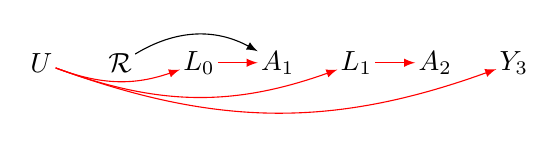
\begin{tikzpicture}
%\node [draw=none, align=center, font=\small] at (.25,1) {\bf Mediator bias};
\node [draw=none, inner sep = 1]  (U) at (0, 0) {$U$};
\node [draw=none, inner sep = 1]  (R) at (1, 0) { $\mathcal{R}$};
\node [rectangle, inner sep = 1] (L0) at (2, 0) {$L_0$};
\node [rectangle, inner sep = 1] (A1) at (3, 0) {$A_1$};
\node [rectangle, inner sep = 1] (L1) at (4, 0) {$L_1$};
\node [rectangle, inner sep = 1] (A2) at (5, 0) {$A_2$};
\node [draw=none, inner sep = 1] (Y3) at (6, 0) {$Y_3$};
\draw [-latex, bend left = 30 ] (R) to (A1);
%\draw [-latex, bend left = 30] (R) to (A2);
\draw [-latex, bend right = 20, red] (U) to (L0);
\draw [-latex, bend right = 20, red] (U) to (L1);
\draw [-latex, bend right = 20, red] (U) to (Y3);
\draw [-latex, red] (L0) to (A1);
\draw [-latex, red] (L1) to (A2);
\end{tikzpicture}
}
\newcommand{\perprotocolTWO}{
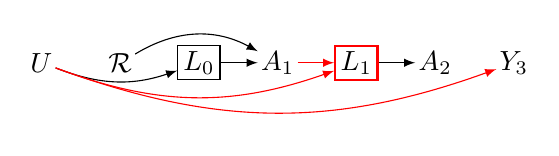
\begin{tikzpicture}
\node [draw=none, inner sep = 1]  (U) at (0, 0) {$U$};
\node [draw=none, inner sep = 1]  (R) at (1, 0) { $\mathcal{R}$};
\node [rectangle, draw = black, inner sep = 2] (L0) at (2, 0) {$L_0$};
\node [rectangle, inner sep = 1] (A1) at (3, 0) {$A_1$};
\node [rectangle, draw = red, inner sep = 2, thick] (L1) at (4, 0) {$L_1$};
\node [rectangle, inner sep = 1] (A2) at (5, 0) {$A_2$};
\node [draw=none, inner sep = 1] (Y3) at (6, 0) {$Y_3$};
\draw [-latex, bend left = 30 ] (R) to (A1);
\draw [-latex, bend right = 20, black] (U) to (L0);
\draw [-latex, bend right = 20, red] (U) to (L1);
\draw [-latex, bend right = 20, red] (U) to (Y3);
\draw [-latex, black] (L0) to (A1);
\draw [-latex, black] (L1) to (A2);
\draw [-latex, red] (A1) to (L1);
\end{tikzpicture}
}
\newcommand{\perprotocolTWOS}{
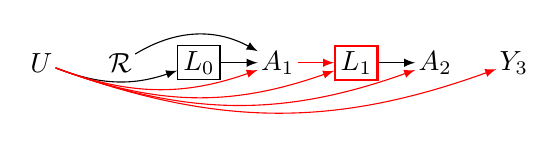
\begin{tikzpicture}
\node [draw=none, inner sep = 1]  (U) at (0, 0) {$U$};
\node [draw=none, inner sep = 1]  (R) at (1, 0) { $\mathcal{R}$};
\node [rectangle, draw = black, inner sep = 2] (L0) at (2, 0) {$L_0$};
\node [rectangle, inner sep = 1] (A1) at (3, 0) {$A_1$};
\node [rectangle, draw = red, inner sep = 2, thick] (L1) at (4, 0) {$L_1$};
\node [rectangle, inner sep = 1] (A2) at (5, 0) {$A_2$};
\node [draw=none, inner sep = 1] (Y3) at (6, 0) {$Y_3$};
\draw [-latex, bend left = 30 ] (R) to (A1);
\draw [-latex, bend right = 20, black] (U) to (L0);
\draw [-latex, bend right = 20, red] (U) to (A1);
\draw [-latex, bend right = 20, red] (U) to (L1);
\draw [-latex, bend right = 20, red] (U) to (A2);
\draw [-latex, bend right = 20, red] (U) to (Y3);
\draw [-latex, black] (L0) to (A1);
\draw [-latex, black] (L1) to (A2);
\draw [-latex, red] (A1) to (L1);
\end{tikzpicture}
}
\newcommand{\mediation}{A \to \boxed{L} \rightarrowdotted Y}
\newcommand{\xandx}{
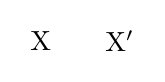
\begin{tikzpicture}
\node [draw=none, inner sep = 1](A) at (0, 0) {X};
\node [draw=none, inner sep = 1] (Y) at (1, 0) {X$^\prime$};
\draw [-latex, draw = white] (A) to (Y);
\end{tikzpicture}
}
\newcommand{\xorx}{
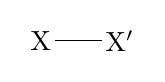
\begin{tikzpicture}
\node [draw=none, inner sep = 1] (A) at (0, 0) {X};
\node [draw=none, inner sep = 1]  (Y) at (1, 0) {X$^{\prime}$};
\draw [draw = black] (A) to (Y);
\end{tikzpicture}
}
\newcommand{\xorxA}{
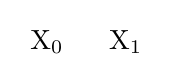
\begin{tikzpicture}
\node [draw=none, inner sep = 1] (A) at (0, 0)  {X$_0$};
\node [draw=none, inner sep = 1]  (Y) at (1, 0)  {X$_1$};
\end{tikzpicture}
}
\newcommand{\xorxorx}{
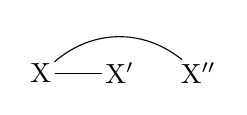
\begin{tikzpicture}
\node [draw=none, inner sep = 1]  (X) at (0, 0) {X};
\node [draw=none, inner sep = 1]  (X1) at (1, 0) {X$^{\prime}$};
\node [draw=none, inner sep = 1] (X2) at (2, 0) {X$^{\prime \prime}$};
\draw [draw = black] (X) to (X1);
\draw [draw = black, bend left = 40] (X) to (X2);
\end{tikzpicture}
}
\newcommand{\xorxchain}{
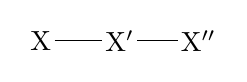
\begin{tikzpicture}
\node [draw=none, inner sep = 1] (X) at (0, 0) {X};
\node [draw=none, inner sep = 1] (X1) at (1, 0) {X$^{\prime}$};
\node [draw=none, inner sep = 1] (X2) at (2, 0) {X$^{\prime \prime}$};
\draw [draw = black] (X) to (X1);
\draw [draw = black] (X1) to (X2);
\end{tikzpicture}
}
\newcommand{\xtox}{
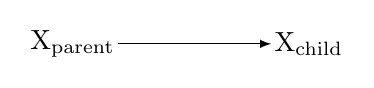
\begin{tikzpicture}
\node [draw=none, inner sep = 1]  (A) at (0, 0)  {X$_\text{parent}$};
\node [draw=none, inner sep = 1]  (Y) at (3, 0)  {X$_\text{child}$};
\draw [-latex, draw = black] (A) to (Y);
\end{tikzpicture}
}
\newcommand{\xtoxA}{
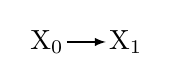
\begin{tikzpicture}
\node [draw=none, inner sep = 1] (A) at (0, 0)  {X$_0$};
\node [draw=none, inner sep = 1]  (Y) at (1, 0)  {X$_1$};
\draw [-latex, draw = black] (A) to (Y);
\end{tikzpicture}
}
\newcommand{\child}{
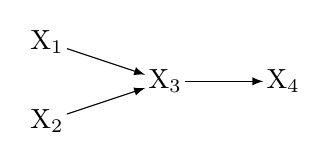
\begin{tikzpicture}
\node [draw=none, inner sep = 1]  (A) at (0, .5) {X$_1$};
\node [draw=none, inner sep = 1]  (L) at (1.5, 0) {X$_3$};
\node [draw=none, inner sep = 1]  (L1) at (3, 0) {X$_4$};
\node [draw=none, inner sep = 1]  (Y) at (0, -.5) {X$_2$};
\draw [-latex, draw = black] (A) to (L);
\draw [-latex, draw = black] (Y) to (L);
\draw [-latex, draw = black] (L) to (L1);
\end{tikzpicture}
}
\newcommand{\fork}{
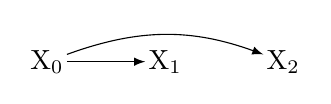
\begin{tikzpicture}
\node [draw=none, inner sep = 1]  (L) at (0, 0) {X$_0$};
\node [draw=none, inner sep = 1]  (A) at (1.5, 0) {X$_1$};
\node [draw=none, inner sep = 1]  (Y) at (3, 0) {X$_2$};
\draw [-latex, draw = black] (L) to (A);
\draw [-latex, draw = white, dotted] (A) to (Y);
\draw [-latex, bend left=20, draw=black] (L) to (Y);
\end{tikzpicture}
}
\newcommand{\chain}{
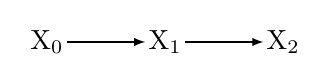
\begin{tikzpicture}
\node [draw=none, inner sep = 1]  (A) at (0, 0) {X$_0$};
\node [draw=none, inner sep = 1] (M) at (1.5, 0) {X$_1$};
\node [draw=none, inner sep = 1]  (Y) at (3, 0) {X$_2$};
\draw [-latex, draw = black] (A) to (M);
\draw [-latex, draw = black] (M) to (Y);
\end{tikzpicture}
}
\newcommand{\immorality}{
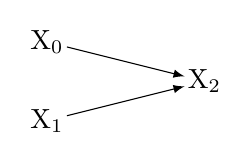
\begin{tikzpicture}
%\node [rectangle, inner sep = 1]  (U) at (0, 0) {};
\node [draw=none, inner sep = 1]  (A) at (1, .5) {X$_0$};
\node [draw=none, inner sep = 1]  (Y) at (1, -.5) {X$_1$};
\node [draw=none, inner sep = 1] (L) at (3, 0) {X$_2$};
\draw [-latex, draw = black] (A) to (L);
\draw [-latex, draw = black] (Y) to (L);
\end{tikzpicture}
}
\newcommand{\network}{
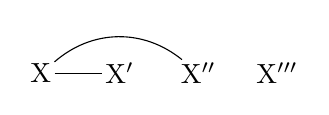
\begin{tikzpicture}
\node [draw=none, inner sep = 1] (X1) at (0, 0) {X};
\node [draw=none, inner sep = 1](X2) at (1, 0) {X$^\prime$};
\node [draw=none, inner sep = 1] (X3) at (2, 0) {X$^{\prime\prime}$};
\node [draw=none, inner sep = 1] (X4) at (3, 0) {X$^{\prime\prime\prime}$};
\draw [draw = black] (X1) to (X2);
\draw [bend left=40, draw=black] (X1) to (X3);
\end{tikzpicture}
}
\newcommand{\aandy}{
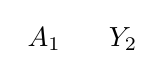
\begin{tikzpicture}
\node [draw=none, inner sep = 0]  (A) at (0, 0) {$A_1$};
\node [draw=none, inner sep = 0]  (Y) at (1, 0) {$Y_2$};
%\node [draw=none, align=center, font=\tiny] at (1.5,.4) {A and Y are not causally associated};
\draw [-latex, draw = white] (A) to (Y);
\end{tikzpicture}
}
\newcommand{\aandyASSERTED}{
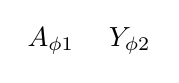
\begin{tikzpicture}
\node [draw=none, inner sep = 0]  (A) at (0, 0) {$A_{\customphi{1}}$};
\node [draw=none, inner sep = 0]  (Y) at (1, 0){$Y_{\customphi{2}}$};
\end{tikzpicture}
}
\newcommand{\aandyASSERTEDLONG}{
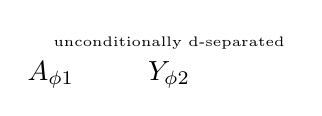
\begin{tikzpicture}
\node [draw=none, inner sep = 0]  (A) at (0, 0) {$A_{\phi{1}}$};
\node [draw=none, inner sep = 0]  (Y) at (1.5, 0){$Y_{\phi{2}}$};
\draw [-latex, draw = white, bend left = 30] (A) to (Y);
\node [draw=none, align=left, font=\tiny] at (1.5,.4) {unconditionally d-separated};
\end{tikzpicture}
}
\newcommand{\atoy}{
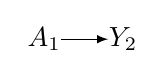
\begin{tikzpicture}
\node [draw=none, inner sep = 0] (A) at (0, 0) {$A_1$};
\node [draw=none, inner sep = 0] (Y) at (1, 0) {$Y_2$};
\draw [-latex, draw = black] (A) to (Y);
%\node [draw=none, align=center, font=\tiny] at (1.25,.4) {A and Y are causally associated};
\end{tikzpicture}
}
\newcommand{\atoyassert}{
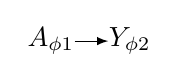
\begin{tikzpicture}
\node [draw=none, inner sep = 0] (A) at (0, 0) {$A_{\phi 1}$};
\node [draw=none, inner sep = 0] (Y) at (1, 0) {$Y_{\phi 2}$};
\draw [-latex, draw = black] (A) to (Y);
%\node [draw=none, align=center, font=\tiny] at (1.25,.4) {A and Y are causally associated};
\end{tikzpicture}
}
\newcommand{\atoyassumed}{
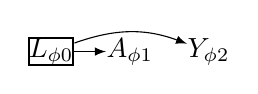
\begin{tikzpicture}
\node [rectangle, draw = black, inner sep = 0, thick] (L) at (0, 0) {$L_{\customphi{0}}$};
\node [draw=none, inner sep = 0] (A) at (1, 0) {$A_{\customphi{1}}$};
\node [draw=none, inner sep = 0] (Y) at (2, 0) {$Y_{\customphi{2}}$};
\draw [-latex,bend left = 20] (L) to (Y);
\draw [-latex,] (L) to (A);
%\node [draw=none, align=center, font=\tiny] at (1.25,.4) {A and Y are causally associated};
\end{tikzpicture}
}
\newcommand{\atoyassumedtiny}{
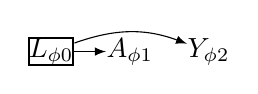
\begin{tikzpicture}
\node [rectangle, draw = black, inner sep = 0, thick] (L) at (0, 0) {$L_{\customphi{0}}$};
\node [draw=none, inner sep = 0] (A) at (1, 0) {$A_{\customphi{1}}$};
\node [draw=none, inner sep = 0] (Y) at (2, 0) {$Y_{\customphi{2}}$};
\draw [-latex,bend left = 20] (L) to (Y);
\draw [-latex,] (L) to (A);
%\node [draw=none, align=center, font=\tiny] at (1.25,.4) {A and Y are causally associated};
\end{tikzpicture}
}
\newcommand{\atoyassumedchild}{
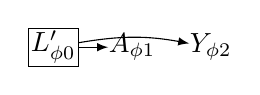
\begin{tikzpicture}
\node [rectangle, draw = black, inner sep =1] (L) at (0, 0) {$L'_{\customphi{0}}$};
\node [draw=none, inner sep = 0] (A) at (1, 0) {$A_{\customphi{1}}$};
\node [draw=none, inner sep = 0] (Y) at (2, 0) {$Y_{\customphi{2}}$};
\draw [-latex,bend left = 10] (L) to (Y);
\draw [-latex,] (L) to (A);
%\node [draw=none, align=center, font=\tiny] at (1.25,.4) {A and Y are causally associated};
\end{tikzpicture}
}
\newcommand{\atoyLONG}{
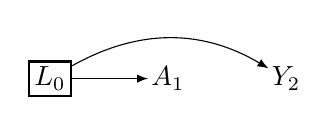
\begin{tikzpicture}
\node [rectangle, draw = black, inner sep = 2, thick](L) at (0, 0) {$L_0$};
\node [draw=none, inner sep = 1] (A) at (1.5, 0) {$A_1$};
\node [draw=none, inner sep = 1] (Y) at (3, 0) {$Y_2$};
\draw [-latex, draw = black] (L) to (A);
\draw [-latex, draw = black, bend left = 30] (L) to (Y);
%\node [draw=none, align=center, font=\tiny] at (1.25,.4) {A and Y are causally associated};
\end{tikzpicture}
}
\newcommand{\abartoy}{
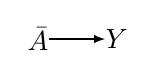
\begin{tikzpicture}
\node [draw=none, inner sep = 0] (A) at (0, 0) {$\bar{A}$};
\node [draw=none, inner sep = 0] (Y) at (1, 0) {$Y$};
\draw [-latex, draw = black] (A) to (Y);
%\node [draw=none, align=center, font=\tiny] at (1.25,.4) {A and Y are causally associated};
\end{tikzpicture}
}
\newcommand{\immoralityChild}{
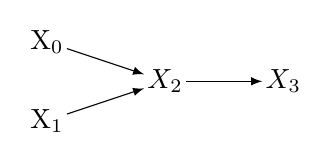
\begin{tikzpicture}
\node [draw = none, inner sep = 1] (A) at (0, .5) {X$_0$};
\node [draw = none, inner sep = 1] (Y) at (0, -.5) {X$_1$};
\node [draw = none, inner sep = 1] (L) at (1.5, 0) {$X_2$};
\node [draw = none, inner sep = 1] (L1) at (3, 0) {$X_3$};
\draw [-latex, draw = black] (A) to (L);
\draw [-latex, draw = black] (Y) to (L);
\draw [-latex, draw = black] (L) to (L1);
\end{tikzpicture}
}
\newcommand{\atoybiased}{
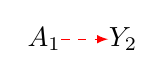
\begin{tikzpicture}
\node [draw=none, inner sep = 0]  (A) at (0, 0) {$A_1$};
\node [draw=none, inner sep = 0]  (Y) at (1.0, 0) {$Y_2$};
%\node [draw=none, align=center, font=\tiny] at (1.5,.4) {Bias in causal association of A and Y};
\draw [-latex, draw = red, dashed] (A) to (Y);
\end{tikzpicture}
}
\newcommand{\abartoybiased}{
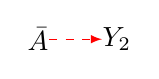
\begin{tikzpicture}
\node [draw=none, inner sep = 0]  (A) at (0, 0) {$\bar{A}$};
\node [draw=none, inner sep = 0]  (Y) at (1.0, 0) {$Y_2$};
%\node [draw=none, align=center, font=\tiny] at (1.5,.4) {Bias in causal association of A and Y};
\draw [-latex, draw = red, dashed] (A) to (Y);
\end{tikzpicture}
}
\newcommand{\ytoa}{
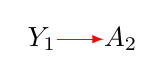
\begin{tikzpicture}
%\node [draw=none, align=center, font=\small] at (0,1) {\bf Timing};
\node [draw=none, inner sep = 0] (Y) at (0, 0) {$Y_1$};
\node [draw=none, inner sep = 0] (A) at (1, 0) {$A_2$};
\draw [-latex, red] (Y) to (A);
\end{tikzpicture}
}
\newcommand{\ytoal}{
\begin{tikzpicture}
%\node [draw=none, align=center, font=\small] at (0,1) {\bf Timing};
\node [draw=rectangle, black, inner sep = 2] (Y) at (0, 0) {$L_0$};
\node [draw=none, inner sep = 0] (Y) at (1.5, 0) {$Y_1$};
\node [draw=none, inner sep = 0] (A) at (3, 0) {$A_2$};
\draw [-latex, red] (Y) to (A);
\draw [-latex, black] (L) to (Y);
\draw [-latex, black, bend left = 30] (L) to (A);
\end{tikzpicture}
}
\newcommand{\atwotoyone}{
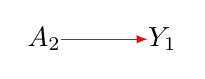
\begin{tikzpicture}
%\node [draw=none, align=center, font=\small] at (0,1) {\bf Timing};
\node [draw=none, inner sep = 0]  (A) at (0, 0) {$A_2$};
\node [draw=none, inner sep = 0]  (Y) at (1.5, 0) {$Y_1$};
\draw [-latex, draw = red] (A) to (Y);
\end{tikzpicture}
}
\newcommand{\commoncause}{
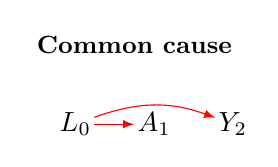
\begin{tikzpicture}
\node [draw=none, align=center, font=\small] at (.75,1) {\bf Common cause};
\node [draw = none, inner sep = 1] (L) at (0, 0) {$L_0$};
\node [draw = none, inner sep = 1] (A) at (1, 0) {$A_1$};
\node [draw = none, inner sep = 1] (Y) at (2, 0) {$Y_2$};
\draw [-latex, draw = red] (L) to (A);
\draw [-latex, draw = white, dotted] (A) to (Y);
\draw [-latex, bend left=20, draw=red] (L) to (Y);
\end{tikzpicture}
}
\newcommand{\commoncauseA}{
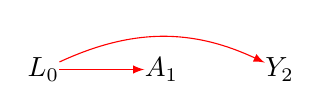
\begin{tikzpicture}
%\node [draw=none, align=center, font=\small] at (.75,1) {\bf Common cause};
\node [draw=none, inner sep = 0] (L) at (0, 0) {$L_0$};
\node [draw=none, inner sep = 0] (A) at (1.5, 0) {$A_1$};
\node [draw=none, inner sep = 0] (Y) at (3, 0) {$Y_2$};
\draw [-latex, draw = red] (L) to (A);
\draw [-latex, draw = white, dotted] (A) to (Y);
\draw [-latex, bend left=25, draw=red] (L) to (Y);
\end{tikzpicture}
}
\newcommand{\commoncauseAASERTED}{
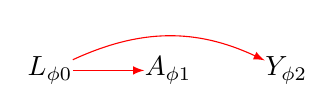
\begin{tikzpicture}
%\node [draw=none, align=center, font=\small] at (.75,1) {\bf Common cause};
\node [draw=none, inner sep = 0] (L) at (0, 0) {$L_{\phi 0}$};
\node [draw=none, inner sep = 0] (A) at (1.5, 0) {$A_{\phi 1}$};
\node [draw=none, inner sep = 0] (Y) at (3, 0) {$Y_{\phi 2}$};
\draw [-latex, draw = red] (L) to (A);
\draw [-latex, bend left=25, red] (L) to (Y);
\end{tikzpicture}
}
\newcommand{\commoncauseUL}{
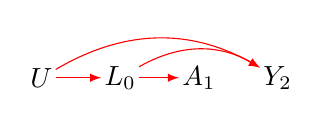
\begin{tikzpicture}
%\node [draw=none, align=center, font=\small] at (.25,1) {\bf Condition on pre-exposure L$^\prime$};
\node [draw=none, align=center, inner sep = 1](U) at (-1, 0) {$U$};
\node [draw=none, align=center, inner sep = 1] (L) at (0, 0) {$L_0$};
\node [draw=none, align=center, inner sep = 1] (A) at (1, 0) {$A_1$};
\node [draw=none, align=center, inner sep = 1] (Y) at (2, 0) {$Y_2$};
\draw [-latex, red] (U) to (L);
\draw [-latex, red] (L) to (A);
\draw [-latex, red, bend left = 30] (L) to (Y);
\draw [-latex, red, bend left = 30] (U) to (Y);
\end{tikzpicture}
}
\newcommand{\commoncauseAshort}{
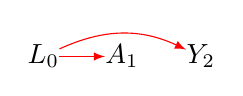
\begin{tikzpicture}
\node [draw=none, inner sep = 0] (L) at (0, 0) {$L_0$};
\node [draw=none, inner sep = 0] (A) at (1, 0) {$A_1$};
\node [draw=none, inner sep = 0] (Y) at (2, 0) {$Y_2$};
\draw [-latex, draw = red] (L) to (A);
\draw [-latex, draw = white, dotted] (A) to (Y);
\draw [-latex, bend left=25, draw=red] (L) to (Y);
\end{tikzpicture}
}
\newcommand{\commoncauseAsupershort}{
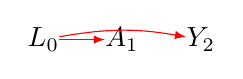
\begin{tikzpicture}
\node [draw=none, inner sep = 0] (L) at (0, 0) {$L_0$};
\node [draw=none, inner sep = 0] (A) at (1, 0) {$A_1$};
\node [draw=none, inner sep = 0] (Y) at (2, 0) {$Y_2$};
\draw [-latex, draw = red] (L) to (A);
\draw [-latex, draw = white, dotted] (A) to (Y);
\draw [-latex, bend left=10, draw=red] (L) to (Y);
\end{tikzpicture}
}
% \newcommand{\commoncauseAA}{
% \begin{tikzpicture}
% %\node [draw=none, align=center, font=\small] at (.75,1) {\bf Common cause};
% \node [draw=none, inner sep = 0] (L) at (0, 0) {$L_0$};
% \node [draw=none, inner sep = 0] (A) at (1.5, 0) {$A_1$};
% \node [draw=none, inner sep = 0] (Y) at (3, 0) {$Y_2$};
% \draw [-latex, draw = red] (L) to (A);
% \draw [-latex, draw = red, dashed] (A) to (Y);
% \draw [-latex, bend left=20, draw=red] (L) to (Y);
% \end{tikzpicture}
% }
\newcommand{\commoncauseALATENTshort}{
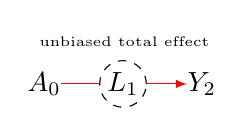
\begin{tikzpicture}
%\node [draw=none, align=center, font=\small] at (1.25,1) {\bf Condition on pre-exposure L};
\node [draw=none, inner sep = 0]  (A) at (0, 0) {$A_0$};
\node [circle, draw=black, dashed, inner sep = 1] (L) at (1, 0) {$L_1$};
\node [draw=none, inner sep = 0]  (Y) at (2, 0) {$Y_2$};
\draw [draw = red] (A) to (L);
\draw [-latex, draw = red] (L) to (Y);
\draw [-latex, bend left=30, draw=white] (A) to node[pos=0.5, above,draw=none, text = black] {\tiny unbiased total effect}(Y);
\end{tikzpicture}
}
\newcommand{\mediator}{
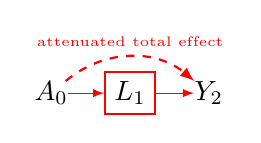
\begin{tikzpicture}
%\node [draw=none, align=center, font=\small] at (.25,1) {\bf Mediator bias};
\node [draw=none, inner sep = 0]  (A) at (0, 0) {$A_0$};
\node [rectangle, draw=red, thick] (L) at (1, 0) {$L_1$};
\node [draw=none, inner sep = 0] (Y) at (2, 0) {$Y_2$};
\draw [-latex, draw = red] (A) to (L);
\draw [-latex, draw = red] (L) to (Y);
\draw [-latex,  bend left=40, draw=red, dashed, thick] (A) to node[pos=0.5, above,draw=none, text = red] {\tiny attenuated total effect} (Y);
\end{tikzpicture}
}
\newcommand{\mediatorA}{
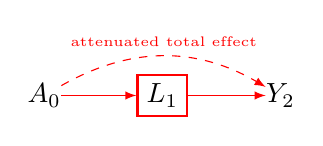
\begin{tikzpicture}
%\node [draw=none, align=center, font=\small] at (.25,1) {\bf Mediator bias};
\node [draw=none, inner sep = 0](A) at (0, 0) {$A_0$};
\node [rectangle, draw=red, thick] (L) at (1.5, 0) {$L_1$};
\node [draw=none, inner sep = 0] (Y) at (3, 0) {$Y_2$};
\draw [-latex, draw = red] (A) to (L);
\draw [-latex, draw = red] (L) to (Y);
\draw [-latex,  bend left=30, draw=red,dashed] (A) to node[pos=0.5, above,draw=none, text = red] {\tiny attenuated total effect} (Y);
\end{tikzpicture}
}
\newcommand{\mediatorAASERTED}{
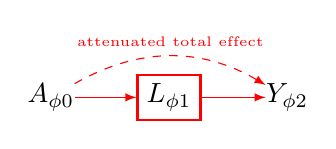
\begin{tikzpicture}
%\node [draw=none, align=center, font=\small] at (.25,1) {\bf Mediator bias};
\node [draw=none, inner sep = 0](A) at (0, 0) {$A_{\phi 0}$};
\node [rectangle, draw=red, thick] (L) at (1.5, 0) {$L_{\phi 1}$};
\node [draw=none, inner sep = 0] (Y) at (3, 0) {$Y_{\phi 2}$};
\draw [-latex, draw = red] (A) to (L);
\draw [-latex, draw = red] (L) to (Y);
\draw [-latex,  bend left=30, draw=red,dashed] (A) to node[pos=0.5, above,draw=none, text = red] {\tiny attenuated total effect} (Y);
\end{tikzpicture}
}
\newcommand{\mediatorAX}{
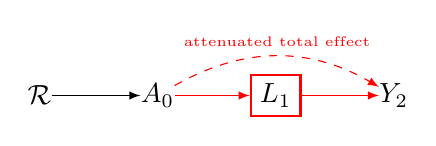
\begin{tikzpicture}
%\node [draw=none, align=center, font=\small] at (.25,1) {\bf Mediator bias};
\node [draw=none, inner sep = 0](R) at (0, 0) { $\mathcal{R}$};
\node [draw=none, inner sep = 0](A) at (1.5, 0) {$A_0$};
\node [rectangle, draw=red, thick] (L) at (3, 0) {$L_1$};
\node [draw=none, inner sep = 0] (Y) at (4.5, 0) {$Y_2$};
\draw [-latex] (R) to (A);
\draw [-latex, draw = red] (A) to (L);
\draw [-latex, draw = red] (L) to (Y);
\draw [-latex,  bend left=30, draw=red,dashed] (A) to node[pos=0.5, above,draw=none, text = red] {\tiny attenuated total effect} (Y);
\end{tikzpicture}
}
\newcommand{\collider}{
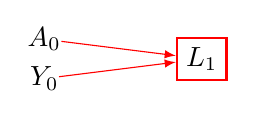
\begin{tikzpicture}
%\node [draw=none, align=center, font=\small] at (0,.75) {\bf Collider};
\node [draw=none, inner sep = 0]  (A) at (0, .25) {$A_0$};
\node [rectangle,  draw=red, thick] (L) at (2, 0) {$L_1$};
\node [draw=none, inner sep = 0]  (Y) at (0, -.25) {$Y_0$};
\draw [-latex, draw = red] (A) to (L);
\draw [-latex, draw = red] (Y) to (L);
\end{tikzpicture}
}
\newcommand{\colliderA}{
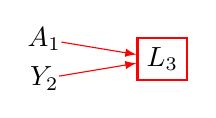
\begin{tikzpicture}
%node [draw=none, align=center, font=\small] at (0,.75) {\bf Collider};
\node [draw=none, inner sep = 0]  (A) at (0, .25) {$A_1$};
\node [rectangle,  draw=red, thick] (L) at (1.5, 0) {$L_3$};
\node [draw=none, inner sep = 0] (Y) at (0, -.25) {$Y_2$};
\draw [-latex, draw = red] (A) to (L);
\draw [-latex, draw = red] (Y) to (L);
\end{tikzpicture}
}
\newcommand{\colliderALONG}{
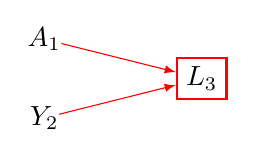
\begin{tikzpicture}
%node [draw=none, align=center, font=\small] at (0,.75) {\bf Collider};
\node [draw=none, inner sep = 0]  (A) at (0, .5) {$A_1$};
\node [rectangle,  draw=red, thick] (L) at (2, 0) {$L_3$};
\node [draw=none, inner sep = 0] (Y) at (0, -.5) {$Y_2$};
\draw [-latex, draw = red] (A) to (L);
\draw [-latex, draw = red] (Y) to (L);
\end{tikzpicture}
}
\newcommand{\descendantB}{
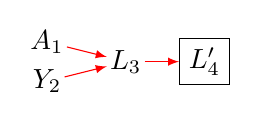
\begin{tikzpicture}
%\node [draw=none, align=center, font=\small] at (1.5,.75) {\bf Descendant of collider};
\node [draw = none, inner sep = 1] (A) at (0, .25) {$A_1$};
\node [draw = none, inner sep = 1] (L) at (1, 0) {$L_3$};
\node [rectangle, draw=black] (L1) at (2, 0) {$L'_4$};
\node [draw = none, inner sep = 1] (Y) at (0, -.25) {$Y_2$};
\draw [-latex, draw = red] (A) -- (L);
\draw [-latex, draw = red] (Y) -- (L);
\draw [-latex, draw = red] (L) -- (L1);
\end{tikzpicture}
}
\newcommand{\descendantBB}{
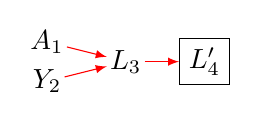
\begin{tikzpicture}
%\node [draw=none, align=center, font=\small] at (1.5,.75) {\bf Descendant of collider};
\node [draw = none, inner sep = 1] (A) at (0, .25) {$A_1$};
\node [draw = none, inner sep = 1] (L) at (1, 0) {$L_3$};
\node [rectangle, draw=black] (L1) at (2, 0) {$L'_4$};
\node [draw = none, inner sep = 1] (Y) at (0, -.25) {$Y_2$};
\draw [-latex, draw = red] (A) -- (L);
\draw [-latex, draw = red] (Y) -- (L);
\draw [-latex, draw = red] (L) -- (L1);
\end{tikzpicture}
}

\newcommand{\descendantBBLONG}{
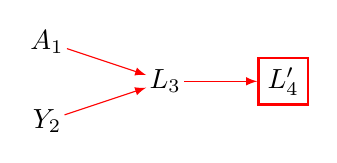
\begin{tikzpicture}
%\node [draw=none, align=center, font=\small] at (1.5,.75) {\bf Descendant of collider};
\node [draw = none, inner sep = 1] (A) at (0, .5) {$A_1$};
\node [draw = none, inner sep = 1] (Y) at (0, -.5) {$Y_2$};
\node [draw = none, inner sep = 1] (L) at (1.5, 0) {$L_3$};
\node [rectangle, draw=red, thick] (L1) at (3, 0) {$L'_4$};
\draw [-latex, draw = red] (A) -- (L);
\draw [-latex, draw = red] (Y) -- (L);
\draw [-latex, draw = red] (L) -- (L1);
\end{tikzpicture}
}
\newcommand{\mediatorcollider}{
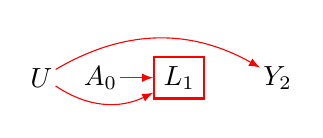
\begin{tikzpicture}
%\node [draw=none, align=center, font=\small] at (2,1) {\bf Condition on child of collider};
\node [draw = none, inner sep = 1] (U) at (0, 0) {$U$};
\node [draw = none, inner sep = 1] (A) at (.75, 0) {$A_{0}$};
\node [rectangle, draw=red, thick](L) at (1.75, 0) {$L_{1}$};
\node [draw = none, inner sep = 1] (Y) at (3, 0) {$Y_{2}$};
\draw [-latex, bend right=30, draw = red] (U) to (L);
\draw [-latex, bend left = 30, draw=red] (U) to (Y);
\draw [-latex,draw=red] (A) to (L);
\end{tikzpicture}
}
\newcommand{\mediatorcolliderX}{
\begin{tikzpicture}
%\node [draw=none, align=center, font=\small] at (2,1) {\bf Condition on child of collider};
\node [draw = none, inner sep = 1] (U) at (0, 0) {$U$};
\node [draw = none, inner sep = 1] (R) at (1, 0) { $\mathcal{R}$};
\node [draw = none, inner sep = 1] (A) at (2.25, 0) {$A_{0}$};
\node [rectangle, draw=red, thick](L) at (3.5, 0) {$L_{1}$};
\node [draw = none, inner sep = 1] (Y) at (5, 0) {$Y_{2}$};
\draw [-latex] (R) to (A);
\draw [-latex, bend right=30, draw = red] (U) to (L);
\draw [-latex, bend left = 30, draw=red] (U) to (Y);
\draw [-latex,draw=red] (A) to (L);
\end{tikzpicture}
}
\newcommand{\experimentAYcollider}{
\begin{tikzpicture}
%\node [draw=none, align=center, font=\small] at (2,1) {\bf Condition on child of collider};
\node [draw = none, inner sep = 1] (R) at (0, 0) { $\mathcal{R}$};
\node [draw = none, inner sep = 1] (A) at (1.5, 0) {$A_{0}$};
\node [draw = none, inner sep = 1] (Y) at (3, 0) {$Y_{1}$};
\node [rectangle, draw=red, thick](L) at (4.5, 0) {$L_{2}$};
\draw [-latex] (R) to (A);
\draw [-latex,draw=red,  bend left=30] (A) to (L);
\draw [-latex,draw=red] (Y) to (L);
\end{tikzpicture}
}
\newcommand{\experimentAYcolliderU}{
\begin{tikzpicture}
%\node [draw=none, align=center, font=\small] at (2,1) {\bf Condition on child of collider};
\node [draw = none, inner sep = 1] (U) at (0, 0) {$U$};
\node [draw = none, inner sep = 1] (R) at (1, 0) { $\mathcal{R}$};
\node [draw = none, inner sep = 1] (A) at (2, 0) {$A_{0}$};
\node [draw = none, inner sep = 1] (Y) at (3.5, 0) {$Y_{1}$};
\node [rectangle, draw=red, thick](L) at (5, 0) {$L_{2}$};
\draw [-latex] (R) to (A);
\draw [-latex, bend right = 20, draw = red] (U) to (L);
\draw [-latex, bend right = 20, draw=red] (U) to (Y);
\draw [-latex, draw=red,  bend left = 20] (A) to (L);
\end{tikzpicture}
}
\newcommand{\downstreamconfounder}{
\begin{tikzpicture}
%\node [draw=none, align=center, font=\small] at (2.5,1) {\bf Condition on child of unmeasured confounder};
\node [draw=none, inner sep = 1] (U) at (0, 0) {$U_L$};
\node [draw=none, inner sep = 1] (A) at (1, 0) {$A_{1}$};
\node [draw=none, inner sep = 1] (Y) at (2, 0) {$Y_{2}$};
\node [rectangle, draw=black, thick] (L) at (3, 0) {$L^{\prime}_{3}$};
\draw [-latex, bend right=30] (U) to (Y);
\draw [-latex, bend left = 30] (U) to (L);
\draw [-latex] (U) to (A);
\end{tikzpicture}
}
\newcommand{\downstream}{
\begin{tikzpicture}
%\node [draw=none, align=center, font=\small] at (1.25,1) {\bf Unmeasured confounding};
\node [draw=none, inner sep = 1] (U) at (0, 0) {$U$};
\node [draw = none, inner sep = 1](A) at (1.5, 0) {$A_{1}$};
\node [ellipse, draw=white] (Y) at (3, 0) {$Y_{2}$};
\draw [-latex, bend left=25, draw =red] (U) to (Y);
\draw [-latex, draw =red] (U) to (A);
\end{tikzpicture}
}
\newcommand{\mediatorm}{
\begin{tikzpicture}
\node [draw=none,inner sep = 1] (A) at (0, 0) {$A_0$};
\node [rectangle, draw=black, thick] (M) at (1.5, 0) {$M_1$};
\node [draw=none,inner sep = 1] (Y) at (3, 0) {$Y_2$};
\draw [-latex, draw = black] (A) to (M);
\draw [-latex, draw = black] (M) to (Y);
\draw [-latex,  bend left=30, draw=black, dashed, thick] (A) to node[pos=0.5, above, draw=none, text = black] {\small direct effect} (Y);
\end{tikzpicture}
}
\newcommand{\mediatormSHORT}{
\begin{tikzpicture}
\node [draw=none, inner sep = 0]  (A) at (0, 0) {$A_0$};
\node [rectangle, draw=black, thick,inner sep = 1] (M) at (1, 0) {$M_1$};
\node [draw=none, inner sep = 0]  (Y) at (2, 0) {$Y_2$};
\draw [-latex, draw = black] (A) to (M);
\draw [-latex, draw = black] (M) to (Y);
\draw [-latex,  bend left=40, draw=black, dashed] (A) to node[pos=0.5, above, draw=none, text = black] {\tiny direct effect} (Y);
\end{tikzpicture}
}
\newcommand{\mbias}{
\begin{tikzpicture}
%\node [draw=none, align=center, font=\small] at (-.25,1) {\bf M-bias};
\node [draw=none, align=center, inner sep = 1](UA) at (0, -.25) {$U_A$};
\node [draw=none, align=center, inner sep = 1] (UY) at (0, .25) {$U_Y$};
\node [rectangle,  draw=red, thick] (L) at (1, 0) {$L_0$};
\node [draw=none, align=center, inner sep = 1](A) at (2, 0) {$A_1$};
\node [draw=none, align=center, inner sep = 1] (Y) at (3, 0) {$Y_2$};
\draw [-latex, draw = red] (UA) to (L);
\draw [-latex, draw = red] (UY) to (L);
\draw [-latex, draw = red, bend right = 30] (UA) to (A);
\draw [-latex, draw = red, bend left = 30] (UY) to (Y);
\end{tikzpicture}
}
\newcommand{\mbiasdoomed}{
\begin{tikzpicture}
%\node [draw=none, align=center, font=\small] at (1.25,1) {\bf M-bias, L is confounder};
\node [draw=none, align=center, inner sep = 1](UA) at (0, -.25) {$U_A$};
\node [draw=none, align=center, inner sep = 1] (UY) at (0, .25) {$U_Y$};
\node [rectangle,  draw=red, thick] (L) at (1, 0) {$L_0$};
\node [draw=none, align=center, inner sep = 1] (A) at (2, 0) {$A_1$};
\node [draw=none, align=center, inner sep = 1](Y) at (3, 0) {$Y_2$};
\draw [-latex, draw = black] (L) to (A);
\draw [-latex, draw = black, bend left = 30] (L) to (Y);
\draw [-latex, draw = red] (UA) to (L);
\draw [-latex, draw = red] (UY) to (L);
\draw [-latex, draw = red, bend right = 30] (UA) to (A);
\draw [-latex, draw = red, bend left = 30] (UY) to (Y);
\end{tikzpicture}
}
% solutions
\newcommand{\aandysolution}{
\begin{tikzpicture}
%\node [draw=none, align=left, font=\small] at (1.25,1) {\bf Ensure relative timing of A and Y};
\node [draw = none, inner sep = 1] (A) at (0, 0) {$A_1$};
\node [draw = none, inner sep = 1] (Y) at (1.5, 0) {$Y_2$};
\draw [-latex, draw = white] (A) to (Y);
\end{tikzpicture}
}
\newcommand{\commoncausesolved}{
\begin{tikzpicture}
\node [draw=none, align=center, font=\small] at (1.25,1) {\bf Condition on pre-exposure L};
\node [rectangle, draw=black] (L) at (0, 0) {$L_0$};
\node [draw=none, inner sep = 0] (A) at (1, 0) {$A_1$};
\node [draw=none, inner sep = 0]  (Y) at (2, 0) {$Y_2$};
\draw [-latex, draw = black] (L) to (A);
\draw [-latex, draw = white, dotted] (A) to (Y);
\draw [-latex, bend left=30, draw=black] (L) to (Y);
\end{tikzpicture}
}
\newcommand{\forksolved}{
\begin{tikzpicture}
\node [rectangle, draw=black, thin, sep = 0] (L) at (0, 0) {$X_0$};
\node [draw=none, inner sep = 0] (A) at (1, 0) {$X_1$};
\node [draw=none, inner sep = 0]  (Y) at (2, 0) {$X_2$};
\draw [-latex, draw = black] (L) to (A);
\draw [-latex, bend left=20, draw=black] (L) to (Y);
\end{tikzpicture}
}
\newcommand{\commoncausesolvedA}{
\begin{tikzpicture}
%\node [draw=none, align=center, font=\small] at (1.25,1) {\bf Condition on pre-exposure L};
\node [rectangle, draw=black] (L) at (0, 0) {$L_0$};
\node [draw = none, inner sep = 1] (A) at (1.5, 0) {$A_1$};
\node [draw = none, inner sep = 1] (Y) at (3, 0) {$Y_2$};
\draw [-latex, draw = black] (L) to (A);
\draw [-latex, draw = white, dotted] (A) to (Y);
\draw [-latex, bend left=25, draw=black] (L) to (Y);
\end{tikzpicture}
}
\newcommand{\commoncausesolvedAASSERTED}{
\begin{tikzpicture}
%\node [draw=none, align=center, font=\small] at (1.25,1) {\bf Condition on pre-exposure L};
\node [rectangle, draw=black] (L) at (0, 0) {$L_{\phi 0}$};
\node [draw = none, inner sep = 1] (A) at (1.5, 0) {$A_{\phi 1}$};
\node [draw = none, inner sep = 1] (Y) at (3, 0) {$Y_{\phi 2}$};
\draw [-latex, draw = black] (L) to (A);
\draw [-latex, draw = white, dotted] (A) to (Y);
\draw [-latex, bend left=25, draw=black] (L) to (Y);
\end{tikzpicture}
}
\newcommand{\commoncausesolvedAshort}{
\begin{tikzpicture}
%\node [draw=none, align=center, font=\small] at (1.25,1) {\bf Condition on pre-exposure L};
\node [rectangle, draw=black] (L) at (0, 0) {$L_0$};
\node [draw=none, inner sep = 0]  (A) at (1, 0) {$A_1$};
\node [draw=none, inner sep = 0]  (Y) at (2, 0) {$Y_2$};
\draw [-latex, draw = black] (L) to (A);
\draw [-latex, bend left=25, draw=black] (L) to (Y);
\end{tikzpicture}
}
\newcommand{\mbiassolved}{
\begin{tikzpicture}
%\node [draw=none, align=center, font=\small] at (1,1) {\bf Do not condition on L};
\node [draw=none, inner sep = 0]  (UA) at (0, -.25) {$U_A$};
\node [draw=none, inner sep = 0]  (UY) at (0, .25) {$U_Y$};
\node [rectangle,  draw=white, thick] (L) at (1, 0) {$L_0$};
\node [draw = none, inner sep = 1] (A) at (2, 0) {$A_1$};
\node [draw = none, inner sep = 1] (Y) at (3, 0) {$Y_2$};
\draw [-latex, draw = black] (UA) to (L);
\draw [-latex, draw = black] (UY) to (L);
\draw [-latex, draw = black, bend right = 30] (UA) to (A);
\draw [-latex, draw = black, bend left = 30] (UY) to (Y);
\end{tikzpicture}
}
\newcommand{\commoncausesolvedchild}{
\begin{tikzpicture}
%\node [draw=none, align=center, font=\small] at (.25,1) {\bf Condition on pre-exposure L$^\prime$};
\node [draw=none, align=center, inner sep = 1](U) at (-1, 0) {$U_L$};
\node [rectangle, draw=black] (L1) at (0, 0) {$L^{\prime}_0$};
\node [draw=none, align=center, inner sep = 1] (A) at (1, 0) {$A_1$};
\node [draw=none, align=center, inner sep = 1] (Y) at (2, 0) {$Y_2$};
\draw [-latex, draw = black] (U) to (L1);
\draw [-latex, draw = black] (L1) to (A);
\draw [-latex, draw = black, bend left = 30] (U) to (Y);
\end{tikzpicture}
}
\newcommand{\commoncausesolvedchildgeneral}{
\begin{tikzpicture}
%\node [draw=none, align=center, font=\small] at (.25,1) {\bf Condition on pre-exposure L$^\prime$};
\node [draw=none, align=center, inner sep = 1](U) at (-1, 0) {$U_L$};
\node [rectangle, draw=black] (L1) at (0, 0) {$L_0$};
\node [draw=none, align=center, inner sep = 1] (A) at (1, 0) {$A_1$};
\node [draw=none, align=center, inner sep = 1] (Y) at (2, 0) {$Y_2$};
\draw [-latex, draw = black] (U) to (L1);
\draw [-latex, draw = black] (L1) to (A);
\draw [-latex, draw = black, bend left = 30] (L1) to (Y);
\draw [-latex, draw = black, bend left = 30] (U) to (Y);
\end{tikzpicture}
}
\newcommand{\mbiasdoomedsolved}{
\begin{tikzpicture}
%\node [draw=none, font=\small] at (1.25, 1) {\bf Condition on measured child of UA OR UY};
\node [draw=none, align=center, inner sep = 1](UA) at (0, -.5) {$U_A$};
\node [draw=none, align=center, inner sep = 1](UY) at (0, .25) {$U_Y$};
\node [rectangle,  draw=black, inner sep = 2] (L) at (1.5, 0) {$L_0$};
\node [rectangle, draw = black, thick, inner sep = 2] (L1) at (1.5, .5) {$L_{UY}$};
\node [draw=none, align=center, inner sep = 1] (A) at (2.5, 0) {$A_1$};
\node [draw=none, align=center, inner sep = 1] (Y) at (3.5, 0) {$Y_2$};
\draw [-latex, draw = black] (UA) to (L);
\draw [-latex, draw = black] (UY) to (L);
\draw [-latex, draw = black] (L) to (A);
\draw [-latex, draw = black, bend left = 20] (L) to (Y);
\draw [-latex, draw = black, bend right = 10] (UA) to (A);
\draw [-latex, draw = black] (UY) to (L1);
\end{tikzpicture}
}
\newcommand{\effectmodifierA}{
\begin{tikzpicture}
\node [rectangle,  inner sep=4pt,  draw=blue, thick] (Z) at (0,0) {$Z$};
\node [draw = none, inner sep = 1] (A) at (1.5, 0) {$A_1$};
\node [draw = none, inner sep = 1] (Y) at (3, 0) {$Y_2$};
\draw [-latex, draw = blue, bend left = 20] (Z) to (Y);
\draw [-latex, draw = black] (A) to (Y);
\end{tikzpicture}
}
\newcommand{\effectmodifierB}{
\begin{tikzpicture}
\node [circle,  inner sep=4pt,  draw=blue, dashed] (Z) at (0,0) {Z};
\node [draw = none, inner sep = 1] (A) at (1.5, 0) {$A_1$};
\node [draw = none, inner sep = 1] (Y) at (3, 0) {$Y_2$};
\draw [-latex, draw = blue, bend left = 20] (Z) to (Y);
\draw [-latex, draw = black] (A) to (Y);
\end{tikzpicture}
}
\newcommand{\effectmodifierC}{
\begin{tikzpicture}
\node [circle, inner sep=6pt, draw=blue,align=left, thick, dashed] (Z) at (0, 0) {$Z$};
\node [rectangle] (A) at (1.5, 0) {$A_1$};
\node [circle, inner sep=4pt,  thick, dashed, draw = black, text=black] (Y) at (3.5,0) {$Y_2$};
\node [circle, inner sep=2pt, draw=blue, text=black, dashed, thick] (US) at (5.5, 1.5) {$U_{\Delta Z \rightarrowblueB Y'}$};
\node [rectangle, draw=black, thick, red, text=black](YS) at (5.5, 0) {Y$_2^{S=1}$};
\draw [-latex, draw=black] (A) to node[pos=0.5, above, draw=none, text = black] {\tiny target}(Y);
\draw [-latex, draw=red] (Y) to node[pos=0.5, above, draw=none, text = red] {\tiny bias}(YS);
\draw [-latex, draw=black] (US) to (YS);
\draw [-latex,bend left=40, blue] (Z) to (Y);
\end{tikzpicture}
}
%measurement
% \newcommand{\measurementerroruncorrelated}{
% \begin{tikzpicture}
% \node [circle, inner sep=2pt, draw=black, dashed, inner sep = 1] (A) at (0, 0) {$A_1$};
% \node [rectangle, draw=red, inner sep = 2]  (A1) at (0, 1.5) {$A'$};
% \node [circle, inner sep=2pt, draw=black, dashed, inner sep = 1] (Y) at (2, 0) {$Y_2$};
% \node [rectangle, draw=red, inner sep = 2] (Y1) at (2, 1.5) {$Y'$};
% \draw [-latex, draw = red, dashed] (A) to node[pos=0.5, sloped, above, draw=none, text= black] {\tiny error} (A1);
% \draw [-latex, draw = red, dashed] (Y) to node[pos=0.5, sloped, above, draw=none, text= black] {\tiny error} (Y1);
% \draw [-latex, draw = black] (A) to node[pos=0.5, above, draw=none, text= black] {\tiny truth} (Y);
% \draw [-latex, draw = red, dashed, thick] (A1) to node[pos=0.5, sloped, above, draw=none, text=black] {\tiny distorted} (Y1);
% \end{tikzpicture}
% }
\newcommand{\measurementUNCOR}{
\begin{tikzpicture}
\node [circle, inner sep=2pt, draw=white] (UA) at (0, 0) {$U_A$};
\node [circle, inner sep=2pt, draw=black, dashed] (A) at (2, 0) {$A_1$};
\node [rectangle, draw=black,thick] (A1) at (4, 0) {$A'_1$};
\node [draw = none, inner sep = 1] (UY) at (6, 0) {$U_Y$};
\node [circle,  inner sep=2pt, draw=black, dashed] (Y) at (8, 0) {$Y_2$};
\node [rectangle, draw=black, thick] (Y1) at (10, 0) {$Y'_2$};
\draw [-latex, draw = black, bend left = 40] (UA) to (A1);
\draw [-latex, draw = black] (A) to (A1);
\draw [-latex, draw = black] (Y) to (Y1);
\draw [-latex, draw = black, bend left = 40] (UY) to (Y1);
\end{tikzpicture}
}
\newcommand{\measurementUCORB}{
\begin{tikzpicture}
\node [circle, draw=blue, dashed, thick] (UA) at (0, 0) {$U_{A}$};
\node [circle, draw=black, dashed] (A) at (2, 0) {$A_1$};
\node [rectangle, draw=red, thick] (A1) at (4, 0) {$A'_1$};
\node [circle, draw=blue, dashed, thick] (UY) at (6, 0) {$U_{Y}$};
\node [circle, draw=black, dashed] (Y) at (8, 0) {$Y_2$};
\node [rectangle, draw=red, thick] (Y1) at (10, 0) {$Y'_2$};
\draw [-latex, draw = blue, bend left = 40] (UA) to (A1);
\draw [-latex, draw = black] (A) to (A1);
\draw [-latex, draw = black] (Y) to (Y1);
\draw [-latex, draw = blue, bend left = 40] (UY) to (Y1);
\draw [-latex, bend right = 40, draw = black] (A) to node[pos=0.5, below, draw=none] {\tiny target}(Y);
\draw [-latex, bend left = 40, draw = red,  dashed, thick] (A1) to node[pos=0.5, above, draw=none, text= red] {\tiny biased}(Y1);
\end{tikzpicture}
}
\newcommand{\measurementCOR}{
\begin{tikzpicture}
\node [draw = none, inner sep = 1] (U) at (0, 0) {$U_{AY}$};
\node [circle, draw=black, dashed] (A) at (1.25, 0) {$A_1$};
\node [rectangle, draw=red, thick] (A1) at (3, 0) {$A'_1$};
\node [circle, draw=black, dashed] (Y) at (4.5, 0) {$Y_2$};
\node [rectangle, draw=red, thick] (Y1) at (6, 0) {$Y'_2$};
\draw [-latex, draw = red, bend left = 30] (U) to (A1);
\draw [-latex, draw = black] (A) to (A1);
\draw [-latex, draw = red, bend left = 30] (U) to (Y1);
\draw [-latex, draw = black] (Y) to (Y1);
\end{tikzpicture}
}
\newcommand{\measurementDIR}{
\begin{tikzpicture}
\node [draw = none, inner sep = 1] (UA) at (0, 0) {$U_A$};
\node [circle, draw=black, dashed] (A) at (1.5, 0) {$A_1$};
\node [rectangle,draw=red, thick] (A1) at (3, 0) {$A'_1$};
\node [draw = none, inner sep = 1] (UY) at (4.5, 0) {$U_Y$};
\node [circle, draw=black, dashed] (Y) at (6, 0) {$Y_2$};
\node [rectangle, draw=red, thick] (Y1) at (7.5, 0) {$Y'_2$};
\draw [-latex, draw = black,  bend right = 40] (UA) to (A1);
\draw [-latex, draw = red] (A) to (A1);
\draw [-latex, draw = red, bend left = 40] (A) to (UY);
\draw [-latex, draw =black] (Y) to (Y1);
\draw [-latex, draw = red, bend right = 40] (UY) to (Y1);
\end{tikzpicture}
}
\newcommand{\measurementCORDIR}{
\begin{tikzpicture}
\node [draw = none, inner sep = 1] (UAY) at (0, 0) {$U_{AY}$};
\node [draw = none, inner sep = 1] (UA) at (1.5, 0) {$U_A$};
\node [circle, draw=black, dashed] (A) at (3, 0) {$A_1$};
\node [rectangle, draw=red, thick] (A1) at (4.5, 0) {$A'_1$};
\node [draw = none, inner sep = 1] (UY) at (6, 0) {$U_Y$};
\node [circle, draw=black, dashed] (Y) at (7, 0) {$Y_2$};
\node [rectangle, draw=red, thick] (Y1) at (9, 0) {$Y'_2$};
\draw [-latex, draw = red] (UAY) to (UA);
\draw [-latex, draw = red, bend right = 40] (UA) to (A1);
\draw [-latex, draw = red] (A) to (A1);
\draw [-latex, draw = red,bend right = 40] (UY) to (Y1);
\draw [-latex, draw = black] (Y) to (Y1);
\draw [-latex, draw = red, bend left = 40] (A) to (UY);
\draw [-latex, draw = red, bend left = 40] (UAY) to (UY);
\end{tikzpicture}
}
\newcommand{\measurementY}{
\begin{tikzpicture}
\node [circle, draw=black, dashed] (A) at (0, 0) {$A_1$};
\node [circle, draw=black, dashed] (Y) at (1.5, 0) {$Y_2$};
\node [draw = none, inner sep = 1] (UA) at (3, 0) {$U_A$};
\node [rectangle, draw=red, thick] (A1) at (4.5, 0) {$A'$};
\node [draw = none, inner sep = 1] (UY) at (6, 0) {$U_Y$};
\node [rectangle,  draw=red, thick] (Y1) at (7.5, 0) {$Y'$};
\draw [-latex, draw = red] (Y) to (UA);
\draw [-latex, draw = red] (UA) to (A1);
\draw [-latex, draw = black, bend right = 30] (A) to (A1);
\draw [-latex, draw = black] (UY) to (Y1);
\draw [-latex, draw = red, bend left = 30] (Y) to (Y1);
\end{tikzpicture}
}
\newcommand{\measurementUNCORshort}{
\begin{tikzpicture}
\node [draw = none, inner sep = 1] (UA) at (0, 0) {$U_A$};
\node [circle, inner sep=1pt, draw=black, dashed] (A) at (1.5, 0) {$A_1$};
\node [rectangle, draw=black, thick] (A1) at (3, 0) {$A'_1$};
\node [draw = none, inner sep = 1] (UY) at (5, 0) {$U_Y$};
\node [circle,  inner sep=1pt, draw=black, dashed] (Y) at (6.5, 0) {$Y_2$};
\node [rectangle, draw=black, thick] (Y1) at (8, 0) {$Y'_2$};
\draw [-latex, draw = black, bend left = 40] (UA) to (A1);
\draw [-latex, draw = black] (A) to (A1);
\draw [-latex, draw = black] (Y) to (Y1);
\draw [-latex, draw = black, bend left = 40] (UY) to (Y1);
\end{tikzpicture}
}
% \newcommand{\measurementUNCORshortTEST}{
% \begin{tikzpicture}
% \node [circle, inner sep=1pt, draw=black, dashed] (A) at (0, 0) {$A_1$};
% \node [rectangle, draw = black, inner sep = 4, thick] (UA) at (1.5, 0) {$U_A$};
% \node [draw = none, inner sep = 1] (A1) at (3, 0) {$A'_1$};
% \node [circle,  inner sep=1pt, draw=black, dashed] (Y) at (5, 0) {$Y_2$};
% \node [rectangle, draw = black, inner sep = 4, thick](UY) at (6.5, 0) {$U_Y$};
% \node [draw = none, inner sep = 1] (Y1) at (8, 0) {$Y'_2$};
% \draw [-latex, draw = black] (A) to (UA);
% \draw [-latex, draw = black] (UA) to (A1);
% \draw [-latex, draw = black] (Y) to (UY);
% \draw [-latex, draw = black] (UY) to (Y1);
% \end{tikzpicture}
% }
\newcommand{\measurementUCORBshort}{
\begin{tikzpicture}
\node [draw = none, inner sep = 4, dashed] (UA) at (0, 0) {$U_A$};
\node [circle, inner sep=2pt, draw=black, dashed] (A) at (1.5, 0) {$A_1$};
\node [rectangle, draw=black] (A1) at (3, 0) {$A'_1$};
\node [draw = none, inner sep = 4, dashed]  (UY) at (5, 0) {$U_Y$};
\node [circle,  inner sep=2pt, draw=black, dashed] (Y) at (7, 0) {$Y_2$};
\node [rectangle, draw=black] (Y1) at (9, 0) {$Y'_2$};
\draw [-latex, draw = black, bend left = 30] (UA) to (A1);
\draw [-latex, draw = black] (A) to (A1);
\draw [-latex, draw = black] (Y) to (Y1);
\draw [-latex, draw = black, bend left = 30] (UY) to (Y1);
%\draw [-latex, draw = blue, bend right = 30, thick] (UA) to (Y1);
\draw [-latex, bend right = 30, draw = black] (A) to node[pos=0.5, above, draw=none] {\tiny target}(Y);
\draw [-latex, bend left = 30, draw = red,  dashed] (A1) to node[pos=0.5, above, draw=none, text= red] {\tiny biased for target}(Y1);
\end{tikzpicture}
}
% \newcommand{\measurementUCORBshortTEST}{
% \begin{tikzpicture}
% \node [circle, inner sep=1pt, draw=black, dashed] (A) at (0, 0) {$A_1$};
% \node [rectangle, draw = black, inner sep = 4, thick] (UA) at (1.5, 0) {$U_A$};
% \node [draw = none, inner sep = 1] (A1) at (3, 0) {$A'_1$};
% \node [circle,  inner sep=1pt, draw=black, dashed] (Y) at (5, 0) {$Y_2$};
% \node [rectangle, draw = black, inner sep = 4, thick](UY) at (6.5, 0) {$U_Y$};
% \node [draw = none, inner sep = 1] (Y1) at (8, 0) {$Y'_2$};
% \draw [-latex, draw = black] (A) to (UA);
% \draw [-latex, draw = black] (UA) to (A1);
% \draw [-latex, draw = black] (Y) to (UY);
% \draw [-latex, draw = black] (UY) to (Y1);
% \draw [-latex, bend right = 30, draw = black] (A) to node[pos=0.5, above, draw=none] {\tiny target}(Y);
% \draw [-latex, bend left = 30, draw = red,  dashed] (A1) to node[pos=0.5, above, draw=none, text= red] {\tiny biased for target}(Y1);
% \end{tikzpicture}
% }
\newcommand{\measurementCORshort}{
\begin{tikzpicture}
\node [draw = none, inner sep = 1] (U) at (0, 0) {$U_{AY}$};
\node [circle, draw=black, dashed] (A) at (2, 0) {$A_1$};
\node [rectangle, draw=red] (A1) at (4, 0) {$A'_1$};
\node [circle, draw=black, dashed] (Y) at (6, 0) {$Y_2$};
\node [rectangle, draw=red] (Y1) at (9, 0) {$Y'_2$};
\draw [-latex, draw = red, bend left = 30] (U) to (A1);
\draw [-latex, draw = black] (A) to (A1);
\draw [-latex, draw = red, bend left = 30] (U) to (Y1);
\draw [-latex, draw = black] (Y) to (Y1);
\end{tikzpicture}
}
\newcommand{\measurementDIRshort}{
\begin{tikzpicture}
\node [draw = none, inner sep = 1] (UA) at (0, 0) {$U_A$};
\node [circle, draw=black, dashed] (A) at (2, 0) {$A_1$};
\node [rectangle,draw=red] (A1) at (4, 0) {$A'_1$};
\node [draw = none, inner sep = 1] (UY) at (6, 0) {$U_Y$};
\node [circle, draw=black, dashed] (Y) at (7.5, 0) {$Y_2$};
\node [rectangle, draw=red] (Y1) at (9, 0) {$Y'_2$};
\draw [-latex, draw = black,  bend right = 30] (UA) to (A1);
\draw [-latex, draw = red] (A) to (A1);
\draw [-latex, draw = red, bend left = 30] (A) to (UY);
\draw [-latex, draw =black] (Y) to (Y1);
\draw [-latex, draw = red, bend right = 30] (UY) to (Y1);
\end{tikzpicture}
}
\newcommand{\measurementCORDIRshort}{
\begin{tikzpicture}
\node [draw = none, inner sep = 1] (UAY) at (0, 0) {$U_{AY}$};
\node [draw = none, inner sep = 1](UA) at (1.5, 0) {$U_A$};
\node [circle, draw=black, dashed, inner sep = 1] (A) at (3, 0) {$A_1$};
\node [rectangle, draw=red] (A1) at (4.5, 0) {$A'_1$};
\node [draw = none, inner sep = 1] (UY) at (6, 0) {$U_Y$};
\node [circle, draw=black, dashed, inner sep = 1] (Y) at (7.5, 0) {$Y_2$};
\node [rectangle, draw=red] (Y1) at (9, 0) {$Y'_2$};
\draw [-latex, draw = red] (UAY) to (UA);
\draw [-latex, draw = red, bend right = 30] (UA) to (A1);
\draw [-latex, draw = red] (A) to (A1);
\draw [-latex, draw = red,bend right = 30] (UY) to (Y1);
\draw [-latex, draw = black] (Y) to (Y1);
\draw [-latex, draw = red, bend left = 30] (A) to (UY);
\draw [-latex, draw = red, bend left = 30] (UAY) to (UY);
\end{tikzpicture}
}
\newcommand{\measurementYshort}{
\begin{tikzpicture}
\node [circle, draw=black, dashed] (A) at (0, 0) {$A_1$};
\node [circle, draw=black, dashed] (Y) at (1.5, 0) {$Y_2$};
\node [draw = none, inner sep = 1](UA) at (3, 0) {$U_A$};
\node [rectangle, draw=red] (A1) at (4.5, 0) {$A'$};
\node [draw = none, inner sep = 1](UY) at (6.5, 0) {$U_Y$};
\node [rectangle,  draw=red] (Y1) at (8.5, 0) {$Y'$};
\draw [-latex, draw = red] (Y) to (UA);
\draw [-latex, draw = red] (UA) to (A1);
\draw [-latex, draw = black, bend right = 30] (A) to (A1);
\draw [-latex, draw = black] (UY) to (Y1);
\draw [-latex, draw = red, bend left = 20] (Y) to (Y1);
\end{tikzpicture}
}
\newcommand{\effectmodification}{
\begin{tikzpicture}
\node [rectangle,thick, draw=blue] (Z) at (0,0) {Z};
\node [draw = none, inner sep = 1] (A) at (2, 0)  {$A_1$};
\node [draw = none, inner sep = 1] (Y) at (4, 0) {$Y_{2}$};
\draw [-latex, draw=black] (A) to (Y);
\draw [-latex, bend left, draw=blue] (Z) to (Y);
\end{tikzpicture}
}
\newcommand{\effectmodificationLONG}{
\begin{tikzpicture}
\node [rectangle,thick, draw=blue] (Z) at (0,0) {Z};
\node [draw = none, inner sep = 1] (A) at (1.5, 0)  {$A_1$};
\node [draw = none, inner sep = 1] (Y) at (3, 0) {$Y_{2}$};
\draw [-latex, draw=black] (A) to (Y);
\draw [-latex, bend left, draw=blue] (Z) to (Y);
\end{tikzpicture}
}
\newcommand{\effectmodificationSHORT}{
\begin{tikzpicture}
\node [rectangle,thick, draw=blue, inner sep = 2] (Z) at (0,0) {Z};
\node [draw = none, inner sep = 1](A) at (.75, 0)  {$A_1$};
\node [draw = none, inner sep = 1](Y) at (2, 0) {$Y_{2}$};
\draw [-latex, draw=black] (A) to (Y);
\draw [-latex, bend left=30, draw=blue] (Z) to (Y);
\end{tikzpicture}
}
\newcommand{\effectmodificationunconditioned}{
\begin{tikzpicture}
\node [circle, dashed, thick, draw=blue, inner sep = 2] (Z) at (0,0) {$Z$};
\node [draw = none, inner sep = 1](A) at (2, 0) {$A_{1}$};
\node [draw = none, inner sep = 1](Y) at (4, 0) {$Y_{2}$};
\draw [-latex, draw=black] (A) to (Y);
\draw [-latex, bend left, draw=blue] (Z) to (Y);
\end{tikzpicture}
}
\newcommand{\effectmodificationunconditionedSHORT}{
\begin{tikzpicture}
\node [circle, dashed, thick, draw=blue, inner sep = 2] (Z) at (0,0) {$Z$};
\node [draw = none, inner sep = 1] (A) at (.75, 0) {$A_{1}$};
\node [draw = none, inner sep = 1] (Y) at (2, 0) {$Y_{2}$};
\draw [-latex, draw=black] (A) to (Y);
\draw [-latex, bend left=30, draw=blue] (Z) to (Y);
\end{tikzpicture}
}
\newcommand{\randomisation}{
\begin{tikzpicture}
\node [draw = none, inner sep = 1] (R) at (0,0) {$\mathcal{R}$};
\node [draw = none, inner sep = 1] (A) at (.75, 0) {$A_{1}$};
\node [draw = none, inner sep = 1] (Y) at (2, 0) {$Y_{2}$};
\draw [-latex, draw=black] (R) to (A);
\end{tikzpicture}
}
\newcommand{\directeffectmodification}{
\begin{tikzpicture}
\node [rectangle, draw=blue, thick, inner sep = 2] (Z) at (0,0) {$Z$};
\node [draw = none, inner sep = 1] (G) at (1.25, 0) {G};
\node [draw = none, inner sep = 1] (A) at (2.75, 0) {$A_1$};
\node [draw = none, inner sep = 1] (Y) at (4, 0) {$Y_2$};
\draw [-latex, draw=black] (A) to (Y);
\draw [-latex, bend left, draw=blue] (Z) to (Y);
\draw [-latex, draw = black] (Z) to (G);
\end{tikzpicture}
}
\newcommand{\indirecteffectmodification}{
\begin{tikzpicture}
\node [circle, dashed, draw=blue, thick, inner sep = 2] (Z) at (0,0) {$Z$};
\node [rectangle, draw=blue, thick, inner sep = 2] (G) at (1.25, 0) {$G$};
\node [draw = none, inner sep = 1] (A) at (2.75, 0) {$A_1$};
\node [draw = none, inner sep = 1] (Y) at (4, 0) {$Y_2$};
\draw [-latex, draw=black] (A) to (Y);
\draw [-latex, bend left, draw=blue] (Z) to (Y);
\draw [-latex, draw = blue] (Z) to (G);
\end{tikzpicture}
}
\newcommand{\indirecteffectmodificationB}{
\begin{tikzpicture}
\node [draw = none, inner sep = 1] (A) at (0, 0)  {$A_1$};
\node [draw = none, inner sep = 1] (Y) at (1.25, 0) {$Y_2$};
\node [circle, draw=blue, dashed, thick, inner sep = 2] (Z) at (-2,0) {$Z$};
\node [rectangle, draw=black] (G) at (-1, 0) {$G$};
\draw [-latex, draw=black] (A) to (Y);
\draw [-latex, bend left, draw=blue] (Z) to (Y);
\draw [-latex, draw = black] (Z) to (G);
\end{tikzpicture}
}
\newcommand{\collidereffectmodification}{
\begin{tikzpicture}
\node [circle, dashed, thick, draw=blue, inner sep = 2] (Z) at (0, .5) {$Z$};
\node [rectangle, thick, draw=blue, thick] (G) at (0, -.5) {$G$};
\node [rectangle, thick, draw=blue] (B) at (1.5,0) {B};
\node [draw = none, inner sep = 1] (A) at (2.5, 0) {$A_1$};
\node [draw = none, inner sep = 1] (Y) at (4, 0) {$Y_2$};
\draw [-latex, draw=black] (A) to (Y);
\draw [-latex, bend left, draw=blue] (Z) to (Y);
\draw [-latex, draw=blue] (Z) to (B);
\draw [-latex, draw=blue] (G) to (B);
\end{tikzpicture}
}
\newcommand{\childeffectmodification}{
\begin{tikzpicture}
\node [rectangle, thick, draw=blue] (Z) at (0, .5) {$Z$};
\node [rectangle, draw=black] (G) at (0, -.5) {$G$};
\node [rectangle, draw=black] (B) at(1.5,0) {B};
\node [draw = none, inner sep = 1] (A) at (2.5, 0) {$A_1$};
\node [draw = none, inner sep = 1] (Y) at (4, 0) {$Y_2$};
\draw [-latex, draw=black] (A) to (Y);
\draw [-latex, bend left, draw=blue] (Z) to (Y);
\draw [-latex, draw=black] (Z) to (B);
\draw [-latex, draw=black] (G) to (B);
\end{tikzpicture}
}
\renewcommand*{\restriction}{
\begin{tikzpicture}
\node [circle, thick, draw=blue, dashed, thick] (Z) at (0, 0) {Z$^{S=\{0,1\}}$};
\node [draw = none, inner sep = 1] (A) at (2, 0) {A$_1^{S=\{0,1\}}$};
\node [circle, draw=black, dashed, thick] (Y) at (6,0) {Y$_2^{S=\{0,1\}}$};
\node [rectangle, draw=red, thick](YS) at (9, 0) {Y$_2^{S=1}$};
\node [circle, inner sep = 2pt, draw=blue,dashed,thick] (US) at (9,1.5) {$U_{\Delta Z \rightarrowblueB Y'}$};
\draw [-latex, draw = red, dashed, thick] (Y) to  node[pos=0.5, draw=none, above, text= red] {\tiny biased }(YS);
\draw [-latex, bend left=50, draw=blue] (Z) to node[pos=0.5, draw=none, above, text= black] {\tiny } (Y);
\draw [-latex, draw=black] (A) to node[pos=0.5, draw=none, above, text= black] {\tiny target}(Y);
\draw [-latex, draw = blue] (US) to (YS);
\end{tikzpicture}
}
\newcommand*{\restrictionSHORT}{
\begin{tikzpicture}
\node [circle, draw=blue, dashed, thick, inner sep = 2] (Z) at (0, 0) {$Z^S$};
\node [draw = none,  inner sep = 1] (A) at (1, 0) {$A^S$};
\node [circle, draw=black, dashed, thick,  inner sep = 2] (Y) at (2.5,0) {$Y_2^S$};
\node [rectangle, draw=red](YS) at (4.5, 0) {Y$_2^{S=1}$};
\node [circle, inner sep = 1pt, draw=blue, dashed] (US) at (4.5,1.5) {$U_{\Delta Z \rightarrowblueB Y'}$};
\draw [-latex, draw = blue] (US) to (YS);
\draw [-latex, draw = red, dashed, thick] (Y) to (YS);
\draw [-latex, bend left=20, draw=blue] (Z) to  (Y);
\draw [-latex, draw=black] (A) to (Y);
\end{tikzpicture}
}
\newcommand*{\restrictionbaseline}{
\begin{tikzpicture}
\node [circle, thick, draw=blue, dashed, thick, inner sep = 2] (Z) at (0, 0) {$Z^S$};
\node [draw = none, inner sep = 1] (A) at (2, 0) {$A_1^{S = 1}$};
\node [circle, draw=red, dashed, thick,  inner sep = 2] (Y) at (4,0) {$Y_2^{S={0,1}}$};
\node [rectangle, draw=red, thick](YS) at (6, 0) {Y$_2^{S=1}$};
%\node [circle, inner sep = 2pt, draw=blue,dashed,thick] (US) at (6,1.5) {$U_{\Delta Z \rightarrowblueB Y'}$};
\draw [-latex, draw = black] (Y) to  (YS);
\draw [-latex, bend left=40, draw=blue] (Z) to (Y);
\draw [-latex, draw=red, dashed, bend left = 40] (A) (YS);
%\draw [-latex, draw = blue] (US) to (YS);
\end{tikzpicture}
}
\newcommand*{\restrictionbaselineSHORT}{
\begin{tikzpicture}
\node [circle, thick, draw=blue, dashed, thick, inner sep = 2] (Z) at (0, -1.5) {$Z^S$};
\node [circle,  draw=blue, dashed, thick, inner sep = 2] (ZS) at (0, 0) {$Z^{S=1}$};
\node [circle,  draw=blue, dashed, inner sep = 1] (UZ) at (0, 1.5) {$U_Z$};
\node [circle, draw=black, dashed, inner sep = 1] (A) at (1.5, -1.5) {$A_1^{S}$};
\node [rectangle, draw=red, inner sep = 1]  (AS) at (1.5, 0) {$A_1^{S = 1}$};
\node [circle,  draw=blue, dashed, inner sep = 1] (UA) at (1.5, 1.5) {$U_A$};
\node [circle, draw=black, dashed, inner sep = 1] (Y) at (3,-1.5) {$Y_2^S$};
\node [rectangle, draw=red, inner sep = 1] (YS) at (3, 0) {Y$_2^{S=1}$};
\node [circle, inner sep = 0pt, draw=blue, dashed] (UY) at (3,1.5) {$U_Y$};
\draw [-latex, draw = black] (UZ) to  (ZS);
\draw [-latex, draw = black] (UA) to  (AS);
\draw [-latex, draw = blue] (UY) to (YS);
\draw [-latex, draw = black] (Z) to  (ZS);
\draw [-latex, draw = black] (A) to  (AS);
\draw [-latex, draw = black] (Y) to  (YS);
\draw [-latex, draw = black] (A) to (Y);
\draw [-latex, draw = red, dashed] (AS) to (YS);
\draw [-latex, bend right=40, draw=blue] (Z) to (Y);
\draw [-latex, bend left=40, draw=blue] (UZ) to (UY);
\end{tikzpicture}
}
\newcommand*{\restrictionbaselineSHORTCORDIR}{
\begin{tikzpicture}
\node [circle, thick, draw=blue, dashed, thick, inner sep = 2] (Z) at (0, -1.5) {$Z^S$};
\node [circle,  draw=blue, dashed, thick, inner sep = 2] (ZS) at (0, 0) {$Z^{S=1}$};
\node [circle,  draw=blue, dashed, inner sep = 1] (UZ) at (0, 1.5) {$U_Z$};
\node [circle, draw=black, dashed, inner sep = 1] (A) at (1.25, -1.5) {$A_1^{S}$};
\node [rectangle, draw=red, inner sep = 1] (AS) at (1.25, 0) {$A_1^{S = 1}$};
\node [circle,  draw=blue, dashed, inner sep = 1] (UA) at (1.25, 1.5) {$U_A$};
\node [circle, draw=black, dashed, inner sep = 1] (Y) at (3,-1.5) {$Y_2^S$};
\node [rectangle, draw=red, inner sep = 1] (YS) at (3, 0) {Y$_2^{S=1}$};
\node [circle, inner sep = 0pt, draw=blue, dashed] (UY) at (3,1.5) {$U_Y$};
\draw [-latex, draw = black] (UZ) to  (ZS);
\draw [-latex, draw = black] (UA) to  (AS);
\draw [-latex, draw = blue] (UY) to (YS);
\draw [-latex, draw = black] (Z) to  (ZS);
\draw [-latex, draw = black] (A) to  (AS);
\draw [-latex, draw = black] (Y) to  (YS);
\draw [-latex, draw = black] (A) to (Y);
\draw [-latex, draw = red, dashed] (AS) to (YS);
\draw [-latex, bend right=40, draw=blue] (Z) to (Y);
\draw [-latex, bend left=40, draw=blue] (UZ) to (UY);
\draw [-latex,  draw=black] (UA) to (UY);
\end{tikzpicture}
}
%targetvalidity
\newcommand*{\restrictionbaselineSHORTCORZ}{
\begin{tikzpicture}
\node [draw = none, inner sep = 0] (UAY) at (0, 0) {$U_{AY}$};
\node [draw = none, inner sep = 0] (UA) at (1.5, 0) {$U_A$};
\node [circle, dashed, draw = black, inner sep = 1] (A) at (3, 0) {$A_1^{}$};
\node [rectangle, draw=red, thick, inner sep = 4](AS) at (4.5, 0) {$A_1^{}$};
\node [draw = none, inner sep = 0] (UY) at (7,0) {$U_Y$};
\node [circle, dashed, draw = black, inner sep = 1] (Y) at (6,0) {$Y_2^{}$};
\node [rectangle, draw=red, thick, inner sep = 4] (YS) at (7.5, 0) {$Y_2^{}$};
\draw [-latex, draw = red, bend right = 30] (UA) to  (AS);
\draw [-latex, draw = red,  bend right = 30] (UY) to (YS);
\draw [-latex, draw = red] (A) to  (AS);
\draw [-latex, draw = red] (Y) to  (YS);
\draw [-latex, draw = black, bend right = 40] (A) to node[pos=0.5, above, draw=none, text= black] {\tiny target ATE}(Y);
\draw [-latex, draw = red, dashed,  bend left = 40, thick] (AS) to node[pos=0.5, above, draw=none, text= red] {\tiny biased ATE for target}(YS);
\draw [-latex, red, bend left = 30] (UAY) to (UA);
\draw [-latex, bend left=40, draw=red] (UAY) to (UY);
\end{tikzpicture}
}
\newcommand{\measurementCORDIRshortCULTURE}{
\begin{tikzpicture}
\node [draw = none, dashed, inner sep = 0] (UAY) at (0, 0) {$U_{AY^{T}}$};
\node [draw = none, inner sep = 0](UA) at (1.0, 0) {$U_A$};
\node [circle, draw=black, dashed, inner sep = 1] (A) at (3, 0) {$A_1$};
\node [rectangle, draw=red] (A1) at (5, 0) {$A^{'}_1$};
\node [draw = none, inner sep = 1] (UY) at (6.5, 0) {$U_Y$};
\node [circle, draw=black, dashed, inner sep = 1] (Y) at (8, 0) {$Y_2$};
\node [rectangle, draw=red, inner sep = 1] (Y1) at (9, 0) {$Y^{'}_2$};
\draw [-latex, draw = red] (UAY) to (UA);
\draw [-latex, draw = red, bend right = 25] (UA) to (A1);
\draw [-latex, draw = black] (A) to (A1);
\draw [-latex, draw = red,bend right = 25] (UY) to (Y1);
\draw [-latex, draw = black] (Y) to (Y1);
%\draw [-latex, draw = red, bend left = 30] (A) to (UY); OPTIONAL directed error
\draw [-latex, draw = red, bend left = 25] (UAY) to  node[pos=0.5, above, draw=none, text= red]{\tiny ambitious target}(UY);
\end{tikzpicture}
}
\newcommand*{\restrictionbaselineCULTURE}{
\begin{tikzpicture}
\node [draw = none, dashed, inner sep = 0] (ULY) at (0, 0) {$U_{LY^{T}}$};
\node [draw = none, inner sep = 0](UL) at (1.5, 0) {$U_L$};
\node [circle, draw=black, dashed] (L) at (2.5, 0) {$L$};
\node [rectangle, draw=red, thick] (L1) at (4, 0) {$L^{'}_1$};
\node [draw = none, inner sep = 1] (A) at (5, 0) {$A_1$};
\node [draw = none, inner sep = 1] (UY) at (6, 0) {$U_Y$};
\node [circle, draw=black, dashed] (Y) at (7.5, 0) {$Y_2$};
\node [rectangle, draw=red, thick] (Y1) at (9, 0) {$Y^{'}_2$};
\draw [-latex, draw = red]  (ULY) to (UL);
\draw [-latex, draw = red, bend right = 25]  (UL) to (L1);
\draw [-latex, draw = red] (L) to (L1);
\draw [-latex, draw = black, bend left = 25] (L) to (A);
\draw [-latex, draw = black, bend left =25]  (L) to (Y);
\draw [-latex, draw = red, bend right = 25] (UY) to (Y1);
\draw [-latex, draw = black] (Y) to (Y1);
\draw [-latex, draw = red, bend left = 25] (ULY) to node[pos=0.5, above, draw=none, text= red]{\tiny ambitious target}(UY);
\end{tikzpicture}
}
\newcommand{\measurementCORDIRshortCULTUREresponse}{
\begin{tikzpicture}
% DO NOT DELETE
%\node [circle, draw = black, dashed, inner sep = 0] (UAY) at (0, 0) {$U_{AY^{T}}$};
\node [draw = none, inner sep = 0](UA) at (0, 0) {$U_A$};
\node [circle, draw=black, dashed, inner sep = 1] (A) at (1.0, 0) {$A_1$};
\node [rectangle, draw=black] (A1) at (3, 0) {$A^{'}_1$};
\node [draw = none, inner sep = 1] (UY) at (4.5, 0) {$U_Y$};
\node [circle, draw=black, dashed, inner sep = 1] (Y) at (5.5, 0) {$Y_2$};
\node [rectangle, draw=black, inner sep = 1] (Y1) at (7.5, 0) {$Y^{'}_2$};
%\draw [-latex, draw = red] (UAY) to (UA);
\draw [-latex, draw = black, bend right = 30] (UA) to (A1);
\draw [-latex, draw = black] (A) to node[pos=0.5, above, draw=none, text= black]{\tiny eligible}(A1);
\draw [-latex, draw = black,bend right = 35] (UY) to  (Y1);
\draw [-latex, draw = black] (Y) to node[pos=0.5, above, draw=none, text= black]{\tiny eligible}(Y1);
%\draw [-latex, draw = red, bend left = 30] (A) to (UY); OPTIONAL directed error
%\draw [-latex, draw = red, bend left = 30] (UAY) to (UY);
\end{tikzpicture}
}
\newcommand*{\restrictionbaselineCULTUREresponse}{
\begin{tikzpicture}
% DO NOT DELETE
%\node [circle, draw = black, dashed, inner sep = 0] (ULY) at (0, 0) {$U_{LY^{T}}$};
\node [draw = none, inner sep = 0](UL) at (0, 0) {$U_L$};
\node [circle, draw=black, dashed] (L) at (1.0, 0) {$L$};
\node [rectangle, draw=black, thick] (L1) at (3, 0) {$L^{'}_1$};
\node [draw = none, inner sep = 1] (A) at (4.5, 0) {$A_1$};
\node [draw = none, inner sep = 1] (UY) at (6, 0) {$U_Y$};
\node [circle, draw=black, dashed] (Y) at (7, 0) {$Y_2$};
\node [rectangle, draw=black, thick] (Y1) at (9, 0) {$Y^{'}_2$};
\draw [-latex, draw = black, bend left =25]  (L) to (Y);
\draw [-latex, draw = black, bend right = 25]  (UL) to (L1);
\draw [-latex, draw = black] (L) to node[pos=0.5, above, draw=none, text= black]{\tiny eligible}(L1);
\draw [-latex, draw = black, bend left = 25] (L) to (A);
\draw [-latex, draw = black, bend right = 25] (UY) to (Y1);
\draw [-latex, draw = black] (Y) to node[pos=0.5, above, draw=none, text= black]{\tiny eligible}(Y1);
%\draw [-latex, draw = red, bend left = 30] (ULY) to (UY);
\end{tikzpicture}
}
\newcommand*{\restrictionbaselineSHORTCOR}{
\begin{tikzpicture}
\node [circle, thick, draw=blue, dashed, thick, inner sep = 2] (Z) at (0, -1.5) {$Z^S$};
\node [circle,  draw=blue, dashed, thick, inner sep = 2] (ZS) at (0, 0) {$Z^{S=1}$};
\node [circle,  draw=blue, dashed, inner sep = 1] (UZ) at (0, 1.5) {$U_Z$};
\node [circle, draw=black, dashed, inner sep = 1] (A) at (1.25, -1.5) {$A_1^{S}$};
\node [rectangle, draw=red, inner sep = 1] (AS) at (1.25, 0) {$A_1^{S = 1}$};
\node [circle,  draw=blue, dashed, inner sep = 1] (UA) at (1.25, 1.5) {$U_A$};
\node [circle, draw=black, dashed, inner sep = 1] (Y) at (3,-1.5) {$Y_2^S$};
\node [rectangle, draw=red, inner sep = 1] (YS) at (3, 0) {Y$_2^{S=1}$};
\node [circle, inner sep = 0pt, draw=blue, dashed] (UY) at (3,1.5) {$U_Y$};
\draw [-latex, draw = black] (UZ) to  (ZS);
\draw [-latex, draw = black] (UA) to  (AS);
\draw [-latex, draw = blue] (UY) to (YS);
\draw [-latex, draw = black] (Z) to  (ZS);
\draw [-latex, draw = black] (A) to  (AS);
\draw [-latex, draw = black] (Y) to  (YS);
\draw [-latex, draw = black] (A) to (Y);
\draw [-latex, draw = red, dashed] (AS) to (YS);
\draw [-latex, bend right=40, draw=blue] (Z) to (Y);
\draw [-latex, bend left=40, draw=blue] (UZ) to (UY);
\end{tikzpicture}
}
\newcommand*{\restrictionbaselineSHORTCORB}{
\begin{tikzpicture}
\node [circle, thick, draw=blue, dashed, thick, inner sep = 2] (Z) at (0, -1.5) {$Z^S$};
\node [circle,  draw=blue, dashed, thick, inner sep = 2] (ZS) at (0, 0) {$Z^{S=1}$};
\node [circle,  draw=blue, dashed, inner sep = 1] (UZAY) at (0, 1.5) {$U_{ZAY}$};
\node [circle, draw=black, dashed, inner sep = 1] (A) at (1.25, -1.5) {$A_1^{S}$};
\node [draw = none, inner sep = 1] (AS) at (1.25, 0) {$A_1^{S = 1}$};
\node [circle, draw=black, dashed, inner sep = 1] (Y) at (3,-1.5) {$Y_2^S$};
\node [rectangle, draw=red, thick](YS) at (3, 0) {Y$_2^{S=1}$};
\draw [-latex, draw = black, bend left = 00] (UZAY) to  (ZS);
\draw [-latex, draw = black, bend left = 20] (UZAY) to  (AS);
\draw [-latex, draw = blue, bend left = 30] (UZAY) to  (YS);
\draw [-latex, draw = black] (Z) to  (ZS);
\draw [-latex, draw = black] (A) to  (AS);
\draw [-latex, draw = black] (Y) to  (YS);
\draw [-latex, draw = black] (A) to (Y);
\draw [-latex, draw = red, dashed] (AS) to (YS);
\draw [-latex, bend right=40, draw=blue] (Z) to (Y);
\end{tikzpicture}
}
\newcommand{\restrictionE}{
\begin{tikzpicture}
\node [draw=none, font = \small]  (S) at (.3, 1.5) {S=$\{0,1\}$};
\node [draw = none, inner sep = 1] (U) at (0, 0) {$U_{AY}$};
\node [circle, inner sep=2pt, draw=black, dashed] (A) at (2, 0) {$A_1$};
\node [rectangle, draw=red, thick] (A1) at (4, 0) {$A'_1$};
\node [circle, inner sep=2pt, draw=black, dashed] (Y) at (6, 0) {$Y_2$};
\node [rectangle, draw=red, thick] (Y1) at (8, 0) {$Y'_2$};
\draw [-latex, draw = red, bend left = 40] (U) to (A1);
\draw [-latex, draw =black] (A) to (A1);
\draw [-latex, draw = red, bend left = 40] (U) to node[pos=0.5, sloped, above, draw=none, text = red]{\tiny Correlated measurement error}(Y1);
\draw [-latex, draw = black] (Y) to (Y1);
\end{tikzpicture}
}
\newcommand{\restrictionF}{
\begin{tikzpicture}
\node [draw=none, font = \small]  (S) at (0, 1) {S=1};
\node [circle, inner sep=2pt, draw=white] (UA) at (0, 0) {$U_A$};
\node [circle, inner sep=2pt, draw=black, dashed] (A) at (2, 0) {$A_1$};
\node [rectangle, draw=black, thick] (A1) at (4, 0) {$A'_1$};
\node [draw = none, inner sep = 1] (UY) at (6, 0) {$U_Y$};
\node [circle, inner sep=2pt, draw=black, dashed] (Y) at (8, 0) {$Y_2$};
\node [rectangle, draw=black, thick] (Y1) at (10, 0) {$Y'_2$};
\draw [-latex, draw = black, bend left = 40] (UA) to (A1);
\draw [-latex, draw = black] (A) to (A1);
\draw [-latex, draw = black] (Y) to (Y1);
\draw [-latex, draw = black, bend left = 40] (UY) to (Y1);
\end{tikzpicture}
}
\newcommand{\restrictionG}{
\begin{tikzpicture}
\node [draw=none, font = \small]  (S) at (-.3, 2.35) {S=$\{0,1\}$};
\node [rectangle, inner sep=4pt, draw=blue, thick] (Z) at (0, 0)  {${ \text{Country}_{Z \rightarrowblueB Y}}$};
\node [rectangle, draw = white] (A) at (3, 0) {$A_1$};
\node [circle, inner sep=2pt, draw=white] (Y) at (8, 0) {$Y_2$};
\draw [-latex, draw = blue, bend left = 30] (Z) to node[pos=0.5, above, draw=none, text = black]{\tiny culture-level heterogeneity} (Y);
\draw [-latex, draw = black] (A) to node[pos=0.5, above, draw=none, text = black]{\tiny ambitious target}(Y);
\end{tikzpicture}
}
\newcommand{\restrictionGG}{
\begin{tikzpicture}
\node [draw=none, font = \small] (S) at (-.5, 2.35) {S=$\{0,1\}$};
\node [circle, inner sep=2pt, draw=blue, thick, dashed] (Z) at (0, 0)  {$ \text{Country}_{Z \rightarrowblueB Y}$};
\node [rectangle, draw = white] (A) at (3, 0) {$A_1$};
\node [circle, inner sep=2pt, draw=white] (Y) at (8, 0) {$Y_2$};
\draw [-latex, draw = blue, bend left = 20] (Z) to node[pos=0.5, above, draw=none, text = black]{\tiny culture-level heterogeneity} (Y);
\draw [-latex, draw = black] (A) to node[pos=0.5, above, draw=none, text = black]{\tiny ambitious target}(Y);
\end{tikzpicture}
}
\newcommand{\restrictionGGG}{
\begin{tikzpicture}
\node [draw=none, font = \small] (S) at (0, 1.35) {S=$\{0,1\}$};
\node [circle, inner sep=2pt, draw=blue, dashed, thick] (U) at (0, 0) {$U_{ZY}$};
\node [rectangle, inner sep=2pt, draw=blue, thick] (Z) at (4, 0)  {$ \text{Country}_{Z \rightarrowblueB Y}$};
\node [rectangle, draw = white] (A) at (6, 0) {$A_1$};
\node [circle, inner sep=2pt, draw=black, dashed] (Y) at (10, 0) {$Y_2$};
\node [rectangle, draw=red, thick] (Y1) at (14, 0) {$Y'_2$};
\draw [-latex, draw = blue] (U) to  node[pos=0.5,above, draw=none, text = black]{\tiny } (Z);
\draw [-latex, draw = blue, bend left = 30, dashed, thick] (U) to  node[pos=0.5,above, draw=none, text = black]{\tiny biased effect-modifier heterogeneity} (Y1);
\draw [-latex, draw = red,  dashed, thick] (Y) to node[pos=0.5, above, draw=none, text = red]{\tiny biased ATE}(Y1);
\draw [-latex, draw = blue, bend right = 20] (Z) to node[pos=0.5, below, draw=none, text = black]{\tiny target ATE} (Y);
\draw [-latex, draw = black] (A) to node[pos=0.5, above, draw=none, text = black]{\tiny target}(Y);
\end{tikzpicture}
}
\newcommand{\restrictionH}{
\begin{tikzpicture}
\node [draw=none, font = \small] (S) at (0, 1) {S=1};
\node [circle, inner sep=4pt, draw=blue, dashed] (Z) at (0, 0) {$Z$};
\node [draw = none, inner sep = 1] (A) at (2, 0) {$A_1$};
\node [draw = none, inner sep = 1] (Y) at (6, 0) {$Y_2$};
\draw [-latex, draw = blue, bend left = 30] (Z) to (Y);
\draw [-latex, draw = black] (A) to node[pos=0.5, above, draw=none, text = black]{\tiny modest target}(Y);
\end{tikzpicture}
}
\newcommand{\attritionB}{
\begin{tikzpicture}
\node [rectangle, draw=white, inner sep = 2, thick] (U1) at (0,1) {U1};
\node [draw = none, inner sep = 1] (U2) at (0,-1) {U2};
\node [rectangle, draw=red, align=left] (S) at (2, 0) {$S = 1$};
\node [draw = none, inner sep = 1] (A) at (4, 0) {$A_{1}$};
\node [draw = none, inner sep = 1] (Y) at (6, 0) {$Y_{2}$};
\draw [-latex, draw=red] (U1) to (S);
\draw [-latex, draw =red] (U2) to (S);
\draw [-latex, draw=red, bend left=30] (U1) to (Y);
\draw [-latex, draw =red, bend right=20] (U2) to (A);
\end{tikzpicture}
}
\newcommand{\attritionBshort}{
\begin{tikzpicture}
% wrong
\node [rectangle, draw=white, inner sep = 1] (U1) at (0,.25) {U1};
\node [draw = none, inner sep = 1] (U2) at (0,-.25) {U2};
\node [rectangle, draw=red, align=left, inner sep =1] (S) at (1, 0) {\footnotesize $S = 1$};
\node [draw = none, inner sep = 1] (R)  at (2, 0) { $\mathcal{R}$};
\node [draw = none, inner sep = 1] (A) at (2.75, 0) {$A_{1}$};
\node [draw = none, inner sep = 1] (Y) at (3.75, 0) {$Y_{2}$};
\draw [-latex, draw=red] (U1) to (S);
\draw [-latex, draw =red] (U2) to (S);
\draw [-latex, draw=red, bend left = 30] (U1) to (Y);
\draw [-latex, draw =red, bend right = 20] (U2) to (R);
\draw [-latex, draw =red] (R) to (A);
\end{tikzpicture}
}
\newcommand{\attritionBB}{
\begin{tikzpicture}
\node [draw = none, inner sep = 1] (U1) at (0,1) {U1};
\node [draw = none, inner sep = 1] (U2) at (0,-1) {U2};
\node [rectangle, draw=black, align=left, inner sep =2] (S) at (2, 0) {\footnotesize $S = 1$};
\node [draw=none, inner sep = 2] (A) at (4, 0) {$A_{1}$};
\node [draw = none, inner sep = 1] (Y) at (6, 0) {$Y_{2}$};
\node [rectangle, draw=black, align=left, inner sep =1] (L) at (3, 1.5) {$L_{0}$};
\draw [-latex, draw=black] (U1) to (S);
\draw [-latex, draw=black,bend left = 15] (U1) to (L);
\draw [-latex, draw =black] (U2) to (S);
\draw [-latex, draw=black, bend left = 10] (L) to (Y);
\draw [-latex, draw =black, bend right = 20] (U2) to (A);
\end{tikzpicture}
}
\newcommand{\attritionBBshort}{
% wrong
\begin{tikzpicture}
\node [rectangle, draw=white, inner sep = 1] (U1) at (0,.25) {U1};
\node [draw = none, inner sep = 1] (U2) at (0,-.25) {U2};
\node [rectangle, draw=black, align=left, inner sep =1] (S) at (1, 0) {\tiny $S = 1$};
\node [draw = none, inner sep = 1] (R)  at (1.75, 0) { $\mathcal{R}$};
\node [draw = none, inner sep = 1] (A) at (2.5, 0) {$A_{1}$};
\node [draw = none, inner sep = 1] (Y) at (3.25, 0) {$Y_{2}$};
\node [rectangle, draw=black, inner sep =1] (L) at (1,0.5) {$L_{0}$};
\draw [-latex, draw=black] (U1) to (S);
\draw [-latex, draw =black] (U2) to (S);
\draw [-latex, draw=black, bend left = 10] (U1) to (L);
\draw [-latex, draw =black, bend right = 20] (U2) to (R);
\draw [-latex, draw=black, bend left = 10] (L) to (Y);
\draw [-latex, draw =black] (R) to (A);
\end{tikzpicture}
}
\newcommand{\mediationfull}{
\begin{tikzpicture}[scale=1] % Adjust the scale factor as needed
\node [draw=none,  align=left, font = \small] (sign) at (3.5, 2.5) {Exposure affects confounder of mediator and outcome};
\node [rectangle, draw=black, thick] (L) at (0, 0) {$L_0$};
\node [rectangle, draw=black, thick] (Q) at (3, 0) {$Q_0$};
\node [ellipse, draw=white] (A) at (6, 0) {$A_{1}$};
\node [rectangle, draw=red, thick](V) at (9, 0) {V$_{2}$};
\node [rectangle, draw = black](M) at (13, 0) {M$_{3}$};
\node [draw = none, inner sep = 1](Y) at (15, 0) {$Y_{4}$};
\draw [-latex, draw=black, bend left = 30] (L) to node [pos=0.5, above, draw=none, text = black] {\tiny confounder $A \to Y$} (A);
\draw [-latex, draw=black, bend right = 30] (L) to node [pos=0.5, above, draw=none, text = black] {\tiny confounder $A \to Y$} (Y);
\draw [-latex, draw=black, bend left = 0] (Q) to  node [pos=0.5, above, draw=none, text = black] {\tiny confounder $A \to M$} (A);
\draw [-latex, draw=black, bend right = 30] (Q) to node [pos=0.5, above, draw=none, text = black] {\tiny confounder $A \to M$} (M);
\draw [-latex, draw= red, bend left = 30,  dashed, thick] (A) to  node [pos=0.5, above, draw=none, text = red] {\tiny biased indirect effect} (M);
\draw [-latex, draw= black, bend left = 50, dashed] (A) to   node[pos=0.5, above, draw=none, text = black]{\tiny direct effect} (Y);
\draw [-latex, draw=red] (A) to  node[pos=0.5, above, draw=none, text = red] {\tiny blocks $A\to M$} (V);
\draw [-latex, draw=red] (V) to node [pos=0.5, above, draw=none, text = red] {\tiny confounder $M \to Y$} (M);
\draw [-latex, draw=black, bend right = 30] (V) to node [pos=0.5, above, draw=none, text = red] {\tiny confounder $M \to Y$} (Y);
\draw [-latex, draw= black] (M) to (Y);
\end{tikzpicture}
}
\newcommand{\feedback}{
\begin{tikzpicture}
\node [draw=none,  align=left, font = \small] (sign) at (4.5, 2) {Exposure 1 affects confounder of Exposure 2: biasing true causality};
\node [rectangle, draw=black] (L0) at (0, 0) {$L_0$};
\node [draw = none, inner sep = 1] (A1) at (2, 0) {$A_{1}$};
\node [draw = none, inner sep = 1] (Y2) at (4, 0) {$Y_{2}$};
\node [rectangle, draw=red, thick] (L3) at (6, 0) {L$_{3}$};
\node [draw = none, inner sep = 1] (A4) at (8, 0) {A$_{4}$};
\node [draw = none, inner sep = 1] (Y5) at (10, 0) {$Y_{5}$};
\draw [-latex,  draw=black] (L0) to (A1);
\draw [-latex,  draw=black,  bend right = 30] (L0) to (Y2);
\draw [-latex,  draw=black] (A1) to (Y2);
\draw [-latex,  draw=red, bend left = 30] (A1) to node[pos=0.8, above, sloped, draw=none, text = red] {\tiny mediator bias}(L3);
\draw [-latex,  draw=black] (L3) to (A4);
\draw [-latex,  draw=red, bend right = 30] (L3) to node[pos=0.5, below, sloped, draw=none, text = red] {\tiny confounder $L_3 \to Y_5$}(Y5);
\draw [-latex,  draw=black] (A4) to (Y5);
\draw [-latex,  draw=red, bend left = 30,  dashed, thick] (A1) to node[pos=0.5, above, draw=none, text = red] {\tiny blocks $A_1 \to Y_5$}(Y5);
\end{tikzpicture}
}
\newcommand{\feedbackINTEREST}{
\begin{tikzpicture}
\node [draw=none, inner sep = 1] (A0) at (0, 0) {$A_{0}$};
%\node [draw=none, inner sep = 0] (Y1) at (1, 0) {Y$_{1}$};
\node [draw=none, inner sep = 1] (A1) at (1.5, 0) {A$_{1}$};
\node [draw=none, inner sep = 1] (Y2) at (3, 0) {Y$_{2}$};
\draw [-latex,  draw=black] (A1) to (Y2);
\draw [-latex,  draw=black, bend left = 30] (A0) to (Y2);
\draw [-latex,  draw=black] (A1) to (Y2);
\end{tikzpicture}
}
\newcommand{\interaction}{
\begin{tikzpicture}
\node [rectangle, draw = black, inner sep = 1](LA) at (0, -.35) {L$_{A_0}$};
\node [rectangle, draw = black,inner sep = 1] (LB) at (0, 0.35) {L$_{B_0}$};
\node [draw=none, inner sep = 1](A) at (1.5, -0.25) {$A_{1}$};
 \node [draw=none, inner sep = 1](B) at (1.5, 0.25) {$B_{1}$};
\node [draw=none, inner sep = 0] (Y) at (3, 0) {$Y_{2}$};
\draw [-latex,  draw=black] (LA) to (A);
\draw [-latex,  draw=black] (LB) to (B);
\draw [-latex,  draw=black, bend right = 30] (LA) to (Y);
\draw [-latex,  draw=black, bend left = 30] (LB) to (Y);
\end{tikzpicture}
}
\newcommand{\feedbackA}{
\begin{tikzpicture}
\node [draw=none,  align=left, font = \small] (sign) at (4.5, 2) {Exposure 1 affects confounder of Exposure 2 when true causality absent};
\node [draw = none, inner sep = 1] (U) at (0, 0) {$U$};
\node [rectangle, draw=black] (L0) at (2, 0) {$L_0$};
\node [draw = none, inner sep = 1] (A1) at (4, 0) {$A_{1}$};
\node [draw = none, inner sep = 1] (Y2) at (6, 0) {$Y_{2}$};
\node [rectangle, draw=red, thick] (L2) at (8, 0) {L$_{3}$};
\node [draw = none, inner sep = 1] (A3) at (10, 0) {A$_{4}$};
\node [draw = none, inner sep = 1] (Y4) at (12, 0) {$Y_{5}$};
\draw [-latex, draw=black] (U) to (L0);
\draw [-latex, draw=black] (L0) to (A1);
\draw [-latex, draw=black] (L2) to (A3);
\draw [-latex, draw=black, bend left = 30] (L2) to node [pos=0.5, above, draw=none, text = red] {\tiny confounder $L_3 \to Y_5$}(Y4);
\draw [-latex, bend left= 30, draw=red] (A1) to node[pos=0.5, above, draw=none, text = red] {\tiny collider}(L2);
\draw [-latex, bend right= 30, draw=black] (U) to (Y2);
\draw [-latex, bend right= 30, draw=red] (U) to node[pos=0.75, above, sloped, draw=none, text = red] {\tiny collider}(L2);
\draw [-latex, bend right= 30, draw=red] (U) to  node[pos=0.5, above, draw=none, text = red] {\tiny fork}(Y4);
\end{tikzpicture}
}
\newcommand{\feedbackB}{
\begin{tikzpicture}
\node [draw=none,  align=left, font = \small] (sign) at (4.5, 2) {Common cause of Exposure 1 and downstream confounder is a collider};
\node [draw=none, inner sep = 1](U1) at (0, 0) {$U_{LY}$};
\node [draw=none, inner sep = 1] (U2) at (0, -1.5) {$U_{AY}$};
\node [rectangle, draw=black] (L0) at (2, 0) {$L_0$};
\node [draw = none, inner sep = 1] (A1) at (4, 0) {$A_{1}$};
\node [draw = none, inner sep = 1] (Y2) at (6, 0) {$Y_{2}$};
\node [rectangle, draw=red, thick] (L2) at (8, 0) {L$_{3}$};
\node [draw = none, inner sep = 1] (A3) at (10, 0) {A$_{4}$};
\node [draw = none, inner sep = 1] (Y4) at (12, 0) {$Y_{5}$};
\draw [-latex, draw=black] (U1) to (L0);
\draw [-latex, draw=black] (L0) to (A1);
\draw [-latex, draw=black] (L2) to (A3);
\draw [-latex, bend left = 30, draw=black] (U1) to (Y2);
\draw [-latex, bend left= 30, draw=red] (U1) to node[pos=0.5, above, draw=none, text = red] {\tiny collider}(L2);
\draw [-latex, bend right= 30, draw=red] (U1) to node[pos=0.5, above, sloped, draw=none, text = red] {\tiny fork}(Y4);
\draw [-latex, draw=red, bend right = 10] (U2) to node[pos=0.5, above, sloped, draw=none, text = red] {\tiny fork/collider}(L2);
\draw [-latex, draw=red] (U2) to node[pos=0.5, above, sloped, draw=none, text = red] {\tiny fork}(A1);
\draw [-latex, draw=black, bend left = 30] (L2) to node [pos=0.5, above, draw=none, text = red] {\tiny confounder $L_3 \to Y_5$}(Y4);
\end{tikzpicture}
}
%threewave
\newcommand{\three}{
\begin{tikzpicture}
\node [rectangle] (U) at (0, 0) {$U$};
\node [rectangle, draw=black,align=left, thick] (L) at (1, 0) {\footnotesize $L_{0}$\\
\footnotesize $A_{0}$\\ \footnotesize $Y_{0}$};
\node [rectangle] (A) at (2.25, 0) {$A_1$};
\node [rectangle, draw=white,text=black] (Y) at (3,0) {$Y_2$};
\draw [-latex] (U) to (L);
% \draw [-latex, bend left=80, red] (U) to  node[pos=0.55, above, draw=none, text = ?, red] {\tiny orthogonal confounding?}(A);
% \draw [-latex, bend right=80, red] (U) to node[pos=0.45, below, draw=none, text = ?, red] {\tiny orthogonal confounding?} (Y);
\draw [-latex] (L) to (A);
\draw [-latex,bend left=20] (L) to (Y);
\end{tikzpicture}
}
\newcommand{\threeB}{
\begin{tikzpicture}
\node [rectangle, draw=black,align=left] (L) at (0, 0) {$L_{0}$\\
$A_{0}$\\ $Y_{0}$};
\node [rectangle] (L1) at (2, 0) {$L_1$};
\node [rectangle] (A) at (4, 0) {$A_1$};
\node [rectangle, draw=white,text=black] (Y) at (6,0) {$Y_2$};
\draw [-latex, bend right = 20] (L) to (A);
\draw [-latex,bend right=20] (L) to (Y);
\draw [-latex, red] (L1) to (A);
\draw [-latex,bend left = 20, red] (L1) to node[pos=0.25, above, draw=none, text = red] {\tiny post-control confounder} (Y);
\end{tikzpicture}
}
\newcommand{\threeC}{
\begin{tikzpicture}
\node [rectangle, draw=black,align=left] (L) at (0, 0) {$L_{0}$\\
$A_{0}$\\ $Y_{0}$};
\node [rectangle] (A) at (2, 0) {$A_1$};
\node [rectangle, draw = red, thick ] (L1) at (4, 0) {$L_1$};
\node [circle, inner sep=2pt, thick, dashed, draw = white, text=black]  (Y) at (6,0) {$Y_2$};
\draw [-latex] (L) to (A);
\draw [-latex,bend right=20] (L) to (Y);
\draw [-latex, red] (A) to (L1);
\draw [-latex, black, bend left = 20, draw=red, dashed, thick] (A) to  node[pos=0.5, above, draw=none, text = red] {\tiny attenuated} (Y);
\draw [-latex, red] (L1) to (Y);
\end{tikzpicture}
}
\newcommand{\threeD}{
\begin{tikzpicture}
\node [draw=none,  align=left, font = \small] (sign) at (1.5, 2) {Missing Completely at Random};
\node [draw=blue, thick, align=left] (L) at (0, 0) {L$_{0}^{S=\{0,1\}}$\\
A$_{0}^{S=\{0,1\}}$\\ Y$_{0}^{S=\{0,1\}}$};
\node [rectangle] (A) at (2.5, 0) {A$_1^{S=\{0,1\}}$};
\node [circle, inner sep=2pt, thick, dashed, draw = black, text=black] (Y) at (5,0) {Y$_2^{S=\{0,1\}}$};
\node [rectangle, draw=white,text=black] (US) at (8,2){$U_{\Delta LAY_0 \rightarrowblueB Y'=0}$};
\draw [-latex, draw=black] (A) to (Y);
\node [rectangle, draw=black](YS) at (8, 0) {$Y_2^{S=1}$};
\draw [-latex, draw=black] (Y) to (YS);
\draw [-latex, draw=black] (US) to (YS);
\draw [-latex] (L) to (A);
\draw [-latex,bend right=20, blue] (L) to (Y);
\end{tikzpicture}
}
\newcommand{\threeE}{
\begin{tikzpicture}
\node [draw=none,  align=left, font = \small] (sign) at (.5, 2) {Missing at Random};
\node [rectangle, draw=blue,align=left, thick] (L) at (0, 0) {L$_{0}^{S=\{0,1\}}$\\
A$_{0}^{S=\{0,1\}}$\\ Y$_{0}^{S=\{0,1\}}$};
\node [rectangle] (A) at (3, 0) {A$_1^{S=\{0,1\}}$};
\node [circle, inner sep=2pt, thick, dashed, draw = black, text=black] (Y) at (6,0) {Y$_2^{S=\{0,1\}}$};
\node [circle, inner sep=2pt, draw=blue,text=black, dashed, thick] (US) at (10,2){$U_{\Delta LAY_0 \rightarrowblueB Y'\ne 0}$};
\node [rectangle, draw=black, thick, red, text=black](YS) at (10, 0) {Y$_2^{S=1}$};
\draw [-latex, draw=black] (A) to node[pos=0.5, above,  draw=none, text = black] {\tiny target}(Y);
\draw [-latex, draw=red,  dashed, thick] (Y) to node[pos=0.5, above, draw=none, text = red] {\tiny biased}(YS);
\draw [-latex, draw=blue] (US) to (YS);
\draw [-latex] (L) to (A);
\draw [-latex,bend right=20, blue] (L) to (Y);
\end{tikzpicture}
}
\newcommand{\threeEE}{
\begin{tikzpicture}
\node [draw=none,  align=left, font = \small] (sign) at (.5, 2) {Missing at Random};
\node [rectangle, draw=blue,align=left, thick] (L) at (0, 0) {$L_{0}$\\
$A_{0}$\\ $Y_{0}$};
\node [rectangle] (A) at (3, 0) {$A_1$};
\node [circle, inner sep=4pt, thick, dashed, draw = black, text=black] (Y) at (6,0){Y$_2^{S=\{0,1\}}$};
\node [circle, inner sep=2pt, draw=blue,text=black, dashed, thick] (US) at (10,2) {$U_{\Delta LAY_0 \rightarrowblueB Y'\ne 0}$};
\node [rectangle, draw=black, thick, red, text=black](YS) at (10, 0) {Y$_2^{S=1}$};
\draw [-latex, draw=black] (A) to  node[pos=0.5, above,  draw=none, text = black] {\tiny target}(Y);
\draw [-latex, draw=red, dashed, thick] (Y) to  node[pos=0.5, above, draw=none, text = red] {\tiny biased}(YS);
\draw [-latex, draw=blue] (US) to (YS);
\draw [-latex] (L) to (A);
\draw [-latex,bend right=30, blue] (L) to (Y);
\end{tikzpicture}
}
\newcommand{\threeEEE}{
\begin{tikzpicture}
\node [draw=none,  align=left, font = \small] (sign) at (-.75, 2) {Not Missing at Random};
\node [circle, inner sep = 4pt, draw=blue, dashed, thick] (Z) at (-2, 0) {$Z_0$};
\node [rectangle, draw=blue,align=left, thick] (L) at (0, 0) {$L_{0}$\\
$A_{0}$\\ $Y_{0}$};
\node [rectangle] (A) at (3, 0) {$A_1$};
\node [circle, inner sep=4pt, thick, dashed, draw = black, text=black] (Y) at (6,0) {Y$_2^{S=\{0,1\}}$};
\node [circle, inner sep=2pt, draw=blue,text=black, dashed, thick] (US) at (10,2) {$U_{\Delta Z \rightarrowblueB Y'\ne 0}$};
\node [rectangle, draw=black, thick, red, text=black](YS) at (10, 0) {Y$_2^{S=1}$};
\draw [-latex, draw=black] (A) to  node[pos=0.5, above,  draw=none, text = black] {\tiny target}(Y);
\draw [-latex, draw=red, dashed, thick] (Y) to  node[pos=0.5, above, draw=none, text = red] {\tiny biased}(YS);
\draw [-latex, draw=blue] (US) to (YS);
\draw [-latex] (L) to (A);
\draw [-latex,bend right=30, blue] (L) to (Y);
\draw [-latex,bend left=40, blue] (Z) to (Y);
\end{tikzpicture}
}
\newcommand{\threeF}{
\begin{tikzpicture}
%\node [draw=none,  align=left, font = \small] (sign) at (4, 3.25) {Unmeasured common cause of exposure and restriction};
\node [draw = none, inner sep = 1] (U) at (0, 0) {$U$};
\node [rectangle, draw=black,align=left, thick] (L) at (2, 0) {L$_{0}^{S=\{0,1\}}$\\
A$_{0}^{S=\{0,1\}}$\\ Y$_{0}^{S=\{0,1\}}$};
\node [rectangle] (A) at (5, 0) {A$_1^{S=\{0,1\}}$};
\node [circle, inner sep=2pt, thick, dashed, draw = black, text=black] (Y) at (7.5,0)  {Y};
\node [rectangle, draw=white,text=black] (US) at (10,3) {$U_{\Delta A \rightarrowred Y'}$};
\node [rectangle, draw=red, thick](YS) at (10, 0) {Y$^{S=1}$};
\draw [-latex, draw = black] (Y) to (YS);
\draw [-latex, draw=red] (US) to (YS);
\draw [-latex, draw=red] (A) to (US);
\draw [-latex, bend left=40, red] (U) to (A);
\draw [-latex] (U) to (L);
\draw [-latex, bend left=20, red] (U) to (US);
\draw [-latex] (L) to (A);
\draw [-latex,bend right=20] (L) to (Y);
\end{tikzpicture}
}
\newcommand{\threeFF}{
\begin{tikzpicture}
\node [draw=none,  align=left, font = \small] (sign) at (4, 3.25) {Unmeasured common cause of exposure and restriction};
\node [draw = none, inner sep = 1] (U) at (0, 0) {$U$};
\node [rectangle, draw=black,align=left, thick] (L) at (2, 0) {$L_{0}$\\ $A_{0}$\\ $Y_{0}$};
\node [draw = none, inner sep = 1] (A) at (5, 0) {$A_1$};
\node [circle, inner sep=4pt, dashed, draw = black] (Y) at (7.5,0)  {Y$_2$};
\node [draw = none, inner sep = 1] (US) at (10,3){$U_{\Delta A \rightarrowred Y'}$};
\node [rectangle, draw=red, thick, inner sep = 1](YS) at (10, 0) {Y$^{S=1}$};
\draw [-latex, black] (Y) to (YS);
\draw [-latex, red] (US) to (YS);
\draw [-latex,red] (A) to (US);
\draw [-latex, bend left=40, red] (U) to (A);
\draw [-latex] (U) to (L);
\draw [-latex, bend left=20, red] (U) to (US);
\draw [-latex] (L) to (A);
\draw [-latex,bend right=20] (L) to (Y);
\end{tikzpicture}
}
\newcommand{\threeG}{
\begin{tikzpicture}
\node [draw=none,  align=left, font = \small] (sign) at (3, 1.5) {Exposure affects restriction};
\node [rectangle, draw=black,align=left] (L) at (2, 0) {L$_{0}^{S=\{0,1\}}$\\
A$_{0}^{S=\{0,1\}}$\\ Y$_{0}^{S=\{0,1\}}$};
\node [rectangle] (A) at (5, 0) {A$_1^{S=\{0,1\}}$};
\node [circle, inner sep=2pt, thick, dashed, draw = black, text=black] (Y) at (9,0)  {Y$_2^{S=\{0,1\}}$};
\node [rectangle, draw=white,text=black] (US) at (12,2){$U_{\Delta A \rightarrowred Y'}$};
\node [rectangle, draw=red, thick](YS) at (12, 0){Y$_2^{S=1}$};
\draw [-latex, draw = black] (Y) to (YS);
\draw [-latex, red, bend left = 18] (A) to (US);
\draw [-latex, draw=red] (US) to (YS);
\draw [-latex] (L) to (A);
\draw [-latex,bend right=20] (L) to (Y);
\end{tikzpicture}
}
\newcommand{\threeGG}{
\begin{tikzpicture}
\node [draw=none,  align=left, font = \small] (sign) at (3, 1.5) {Outcome affects restriction};
\node [rectangle, draw=black,align=left] (L) at (2, 0){$L_{0}$\\ $A_{0}$\\ $Y_{0}$};
\node [rectangle] (A) at (5, 0) {A$_1^{S=\{0,1\}}$};
\node [circle, inner sep=2pt, thick, dashed, draw = black, text=black] (Y) at (9,0)  {Y$_2^{S=\{0,1\}}$};
\node [rectangle, draw=white,text=black] (US) at (12,2){$U_{\Delta A \rightarrowred Y'}$};
\node [rectangle, draw=red, thick](YS) at (12, 0){Y$_2^{S=1}$};
\draw [-latex, draw = black] (Y) to (YS);
\draw [-latex, red, bend left = 35] (Y) to (US);
\draw [-latex, draw=red] (US) to (YS);
\draw [-latex] (L) to (A);
\draw [-latex,bend right=20] (L) to (Y);
\end{tikzpicture}
}
\newcommand{\threeGGA}{
\begin{tikzpicture}
\node [draw=none,  align=left, font = \small] (sign) at (2.5, 1.5) {Exposure affects restriction};
\node [rectangle, draw=black,align=left] (L) at (2, 0) {$L_{0}$\\ $A_{0}$\\ $Y_{0}$};
\node [rectangle] (A) at (5, 0) {$A_1$};
\node [circle, inner sep=2pt, thick, dashed, draw = black, text=black] (Y) at (9,0)  {Y$_2^{S=\{0,1\}}$};
\node [rectangle, draw=white,text=black] (US) at (12,2){$U_{\Delta A \rightarrowred Y'}$};
\node [rectangle, draw=red, thick](YS) at (12, 0){Y$_2^{S=1}$};
\draw [-latex, draw = black] (Y) to (YS);
\draw [-latex, red, bend left = 18] (A) to (US);
\draw [-latex, draw=red] (US) to (YS);
\draw [-latex] (L) to (A);
\draw [-latex,bend right=20] (L) to (Y);
\end{tikzpicture}
}
\newcommand{\threeGGY}{
\begin{tikzpicture}
\node [draw=none,  align=left, font = \small] (sign) at (3, 1.5) {Outcome affects restriction};
\node [rectangle, draw=black,align=left] (L) at (2, 0) {L$_{0}^{S=\{0,1\}}$\\
A$_{0}^{S=\{0,1\}}$\\ Y$_{0}^{S=\{0,1\}}$};
\node [rectangle] (A) at (5, 0) {$A_1$};
\node [circle, inner sep=2pt, thick, dashed, draw = black, text=black] (Y) at (9,0)  {Y$_2^{S=\{0,1\}}$};
\node [rectangle, draw=white,text=black] (US) at (12,2){$U_{\Delta A \rightarrowred Y'}$};
\node [rectangle, draw=red, thick](YS) at (12, 0){Y$_2^{S=1}$};
\draw [-latex, draw = black] (Y) to (YS);
\draw [-latex, red, bend left = 35] (Y) to (US);
\draw [-latex, draw=red] (US) to (YS);
\draw [-latex] (L) to (A);
\draw [-latex,bend right=20] (L) to (Y);
\end{tikzpicture}
}
\newcommand{\threeH}{
\begin{tikzpicture}
\node [draw=none,  align=left, font = \small] (sign) at (3, 1.5) {Distribution of effect-modifiers differs in restricted sample};
\node [circle, inner sep=2pt, thick, draw=blue, dashed, thick] (Z) at (0, 0) {Z$^{S=\{0,1\}}$};
\node [draw = none, inner sep = 1] (A) at (2, 0) {A$_1^{S=\{0,1\}}$};
\node [circle, inner sep=2pt, draw=black, dashed, thick] (Y) at (6,0) {Y$_2^{S=\{0,1\}}$};
\node [rectangle, draw=red, thick](YS) at (9, 0) {Y$_2^{S=1}$};
\node [circle, inner sep=2pt, draw=blue,dashed,thick] (US) at (9,1.5){$U_{\Delta Z \rightarrowblueB Y'}$};
\draw [-latex, draw = red, dashed, thick] (Y) to  node[pos=0.5, draw=none, above, text= black] {\tiny biased }(YS);
\draw [-latex, bend left=30, draw=blue] (Z) to node[pos=0.5, draw=none, above, text= black] {\tiny } (Y);
\draw [-latex, draw=black] (A) to node[pos=0.5, draw=none, above, text= black] {\tiny target}(Y);
\draw [-latex, draw = blue] (US) to (YS);
\end{tikzpicture}
}
%standard dags
% \newcommand{\sdA}{
% \begin{tikzpicture}
% \node [draw=none, align=center, font=\tiny] at (2,1.25) {Treatment affects attrition: standard DAG};
% \node [draw = none, inner sep = 1] (A) at (1, 0) {$A_1$};
% \node [ellipse, draw=white] (U) at (0, 0) {$U$};
% \node [rectangle, draw=red, thick](S) at (2.5, 0) {$S=1$};
% \node [ellipse, draw=white] (Y) at (4, 0) {$Y_2$};
% \draw [-latex, bend left=50, draw=red] (U) to (Y);
% \draw [-latex, draw=red] (A) to (S);
% \draw [-latex, draw=red, bend right=50] (U) to (S);
% \end{tikzpicture}
% }
\newcommand{\sdB}{
\begin{tikzpicture}
\node [draw=none, align=center, font=\tiny] at (1.5,.75) {Common cause of exposure and attrition};
\node [draw = none, inner sep = 1] (U) at (0, 0) {$U_{\Delta Y}$};
\node [draw = none, inner sep = 1] (A) at (2, 0) {$A_{1}$};
\node [draw = none, inner sep = 1] (Y) at (4, 0) {$Y_{2}$};
\node [rectangle, draw=red, thick](YS) at (6, 0) {$Y^{S=1}_{2}$};
\draw [-latex, draw=red, bend right=20] (U) to (YS);
\draw [-latex, draw=red] (U) to (A);
\draw [-latex, draw=black] (Y) to (YS);
\end{tikzpicture}
}
\newcommand{\sdC}{
\begin{tikzpicture}
\node [draw=none, align=center, font=\tiny] at (0.5,.75) {Treatment affects attrition};
\node [draw = none, inner sep = 1] (A) at (0, 0) {$A_{1}$};
\node [draw = none, inner sep = 1] (U) at (2, 0) {$U_{\Delta Y}$};
\node [draw = none, inner sep = 1] (Y) at (4, 0) {$Y^{S=1}_{2}$};
\node [rectangle,  draw=red, thick](YS) at (6, 0) {$Y'_{2}$};
\draw [-latex, draw=red] (A) to (U);
\draw [-latex, draw=red, bend right=20] (U) to (YS);
\draw [-latex, draw=black] (Y) to (YS);
\end{tikzpicture}
}
\newcommand{\sdD}{
\begin{tikzpicture}
\node [draw=none, align=center, font=\tiny] at (3.0,.75) {Outcome affects attrition absent causation};
\node [draw = none, inner sep = 1] (A) at (2, 0) {$A_{1}$};
\node [circle, dashed, inner sep = 2pt, draw=black]  (Y) at (4, 0) {Y};
\node [draw = none, inner sep = 1] (U) at (6, 0) {$U_{\Delta Y}$};
\node [rectangle,  draw=black, thick](YS) at (8, 0) {$Y^{S=1}_{2}$};
\draw [-latex, draw=black] (Y) to (U);
\draw [-latex, draw=black] (U) to (YS);
\end{tikzpicture}
}
\newcommand{\sdDD}{
\begin{tikzpicture}
\node [draw=none, align=center, font=\tiny] at (3.5,.75) {True treatment effects differ in restricted sample};
\node [draw = none, inner sep = 1] (A) at (2, 0) {$A_{1}$};
\node [circle, dashed, inner sep = 2pt, draw=black] (Y) at (4, 0) {Y};
\node [draw = none, inner sep = 1] (U) at (6, 0) {$U_{\Delta Y}$};
\node [rectangle,  draw=red, thick](YS) at (8, 0) {$Y'_{2}$};
\draw [-latex, draw=black] (A) to (Y);
\draw [-latex, draw=red, dashed, thick, bend right = 20] (A) to (YS);
\draw [-latex, draw=red] (Y) to (U);
\draw [-latex, draw=red] (U) to (YS);
\end{tikzpicture}
}
\newcommand{\sdE}{
\begin{tikzpicture}
\node [draw=none, align=center, font=\tiny] at (2,1.25) {Treatment affects attrition: standard DAG};
\node [draw = none, inner sep = 1] (U) at (0, 0) {$U_{\Delta Y}$};
\node [rectangle, draw=black, align=left] (L) at (2, 0) {$L_0$};
\node [draw = none, inner sep = 1] (A) at (4, 0) {$A_{1}$};
\node [rectangle, draw=black](S) at (6, 0) {S=1};
\node [draw = none, inner sep = 1] (Y) at (8, 0) {Y$_{t2}$};
\draw [-latex, draw=black] (U) to (L);
\draw [-latex, draw=red, bend right = 30] (U) to node[pos=0.5, above, draw=none, text = red]{\tiny  collider/fork} (S);
\draw [-latex, draw=red, bend right = 30] (U) to node[pos=0.5, above, draw=none, text = red]{\tiny fork} (Y);
\draw [-latex, draw=black] (L) to (A);
\draw [-latex, bend left=30, draw=black] (L) to (Y);
\draw [-latex, draw=red] (A) to node[pos=0.5, above, draw=none, text = red]{\tiny collider}  (S);
\end{tikzpicture}
}
\newcommand{\sdF}{
\begin{tikzpicture}
\node [draw=none, align=center, font=\tiny] at (2,1.25) {Treatment affects attrition: standard DAG};
\node [ellipse, draw=white] (U) at (0, 0) {$U$};
\node [draw = none, inner sep = 1] (A) at (2, 0) {$A_1$};
\node [draw = none, inner sep = 1](L) at (4, 0) {$L_1$};
\node [rectangle, draw=white,text=black] (US) at (6,0) {$U_{\Delta Y}$};
\node [rectangle, draw=white,text=black] (Y) at (8,0) {$Y_2$};
\node [rectangle, draw=red, thick, fill=red!0](YS) at (10, 0) {Y$_2^{S=1}$};
\draw [-latex, bend left = 30, draw=red] (US) to (YS);
\draw [-latex, draw=red, bend left = 30] (U) to (L);
\draw [-latex, draw=red, bend right = 30] (U) to (Y);
\draw [-latex, draw=red] (A) to (L);
\draw [-latex, draw=red] (L) to (US);
\draw [-latex, draw = black] (Y) to (YS);
\end{tikzpicture}
}
\newcommand{\sdG}{
\begin{tikzpicture}
\node [draw=none, align=center, font=\tiny] at (2,1.25) {Treatment affects attrition: standard DAG};
\node [ellipse, draw=white] (U) at (0, 0) {$U$};
\node [draw = none, inner sep = 1] (A) at (2, 0) {$A_1$};
\node [rectangle, draw=red,thick](L) at (4, 0) {$L_1$};
\node [rectangle, draw=white,text=black] (US) at (6,0){$U_{\Delta Y}$};
\node [rectangle, draw=white,text=black] (Y) at (8,0) {$Y_2$};
\node [rectangle, draw=white, thick, fill=red!0](YS) at (10, 0) {Y$_2^{S=1}$};
\draw [-latex, bend left = 30, draw=red] (US) to (YS);
\draw [-latex, draw=red, bend left = 30] (U) to (L);
\draw [-latex, draw=red, bend right = 30] (U) to (US);
\draw [-latex, draw=red] (A) to (L);
\draw [-latex, draw=black] (L) to (US);
\draw [-latex, draw = black] (Y) to (YS);
\end{tikzpicture}
}
\newcommand{\sdH}{
\begin{tikzpicture}
\node [draw=none, align=center, font=\tiny] at (1.5,1.25) {Common cause of exposure and attrition};
\node [ellipse, draw=white] (U) at (0, 0) {$U$};
\node [draw=none, inner sep = 0] (A) at (2, 0) {$A_1$};
\node [rectangle, draw=white,text=black] (US) at (4,0) {$U_{\Delta Y}$};
\node [draw=none, inner sep = 0] (Y) at (6,0) {$Y_2$};
\node [rectangle, draw=red, thick](YS) at (8, 0) {Y$_2^{S=1}$};
\draw [-latex, draw=red] (U) to (A);
\draw [-latex, draw = black] (Y) to (YS);
\draw [-latex, draw=red,  bend right = 30] (US) to (YS);
\draw [-latex, draw=red, bend left = 30] (U) to (US);
\end{tikzpicture}
}
\newcommand{\sdBshort}{
\begin{tikzpicture}
%\node [draw=none, align=center, font=\tiny] at (1.25,.75) {Common cause of exposure and attrition};
\node [draw = none, inner sep = 1] (U) at (0, 0) {$U_{}$};
\node [draw=none, inner sep = 1] (A) at (2, 0) {$A_{1}$};
\node [circle, dashed, inner sep = 2pt, draw=black]  (Y) at (4, 0) {$Y_{2}$};
\node [rectangle, draw=red, thick](YS) at (6, 0) {$Y^{\prime}_{2}$};
\draw [-latex, draw=red, bend right=30] (U) to (YS);
\draw [-latex, draw=red] (U) to (A);
\draw [-latex, draw=black] (Y) to (YS);
\end{tikzpicture}
}
\newcommand{\sdCshort}{
\begin{tikzpicture}
%\node [draw=none, align=center, font=\tiny] at (0.5,.75) {Treatment affects attrition};
\node [draw = none, inner sep = 1] (A) at (0, 0) {$A_{1}$};
\node [draw=none, inner sep = 1] (U) at (2, 0) {$U_{\Delta Y}$};
\node [circle, dashed, inner sep = 2pt, draw=black] (Y) at (4, 0) {$Y_{2}$};
\node [rectangle,  draw=red, thick](YS) at (6, 0) {$Y^{\prime}_{2}$};
\draw [-latex, draw=red] (A) to (U);
\draw [-latex, draw=red, bend right=30] (U) to (YS);
\draw [-latex, draw=black] (Y) to (YS);
\end{tikzpicture}
}
\newcommand{\sdCshortVERY}{
\begin{tikzpicture}
%\node [draw=none, align=center, font=\tiny] at (0.5,.75) {Treatment affects attrition};
\node [draw = none, inner sep = 1] (A) at (0, 0) {$A_{1}$};
\node [draw=none, inner sep = 1] (U) at (1.25, 0) {$U_{\Delta Y}$};
\node [circle, dashed, inner sep = 2pt, draw=black] (Y) at (2.5, 0) {$Y_{2}$};
\node [rectangle,  draw=red, thick](YS) at (4, 0) {$Y^{\prime}_{2}$};
\draw [-latex, draw=red] (A) to (U);
\draw [-latex, draw=red, bend right=30] (U) to (YS);
\draw [-latex, draw=black] (Y) to (YS);
\end{tikzpicture}
}
\newcommand{\sdCshortVERYX}{
\begin{tikzpicture}
%\node [draw=none, align=center, font=\tiny] at (0.5,.75) {Treatment affects attrition};
\node [draw = none, inner sep = 1] (R) at (0, 0) { $\mathcal{R}$};
\node [draw = none, inner sep = 1] (A) at (1, 0) {$A_{1}$};
\node [draw=none, inner sep = 1] (U) at (2.5, 0) {$U_{\Delta Y}$};
\node [circle, dashed, inner sep = 2pt, draw=black] (Y) at (4, 0) {$Y_{2}$};
\node [rectangle,  draw=red, thick](YS) at (5.75, 0) {$Y^{\prime}_{2}$};
\draw [-latex] (R) to (A);
\draw [-latex, draw=red] (A) to (U);
\draw [-latex, draw=red, bend right=30] (U) to (YS);
\draw [-latex, draw=black] (Y) to (YS);
\end{tikzpicture}
}
\newcommand{\sdDshort}{
\begin{tikzpicture}
%\node [draw=none, align=center, font=\tiny] at (1.25,.75) {Outcome affects attrition absent causation};
\node [draw=none, inner sep = 0]  (A) at (0, 0) {$A_{1}$};
\node [circle, dashed, inner sep = 2pt, draw=black]  (Y) at (2, 0) {$Y_2$};
\node [draw=none, inner sep = 1]  (U) at (4, 0) {$U_{\Delta Y}$};
\node [rectangle,  draw=black, thick](YS) at (6, 0) {$Y^{\prime}_{2}$};
\draw [-latex, draw=black] (Y) to (U);
\draw [-latex, draw=black] (U) to (YS);
\end{tikzpicture}
}
\newcommand{\sdDDshort}{
\begin{tikzpicture}
%\node [draw=none, align=center, font=\tiny] at (2.5,.75) {True treatment effects differ in restricted sample: Y affects restriction};
\node [draw=none, inner sep = 0] (A) at (0, 0) {$A_{1}$};
\node [circle, dashed, inner sep = 2pt, draw=black] (Y) at (2, 0) {$Y_2$};
\node [draw=none, inner sep = 1] (U) at (4, 0) {$U_{\Delta^{A \to Y}}$};
\node [rectangle,  draw=red, thick](YS) at (6, 0) {$Y'_{2}$};
\draw [-latex, draw=black] (A) to (Y);
\draw [-latex, draw=red, dashed,  bend left = 20] (A) to node[pos=0.5, above, draw=none, text= red]{\tiny biased for target} (YS);
\draw [-latex, draw=red] (Y) to (U);
\draw [-latex, draw=red] (U) to (YS);
\end{tikzpicture}
}
\newcommand{\sdHshort}{
\begin{tikzpicture}
%\node [draw=none, align=center, font=\tiny] at (1.5,1.25) {Common cause of exposure and attrition};
\node [draw=none, inner sep = 1]  (U) at (0, 0) {$U$};
\node [draw=none, inner sep = 1] (A) at (2, 0) {$A_1$};
\node [draw=none, inner sep = 1]  (US) at (4,0) {$U_{\Delta Y}$};
\node [circle, dashed, inner sep = 2pt, draw=black] (Y) at (6,0) {$Y_2$};
\node [rectangle, draw=red, thick](YS) at (8, 0) {Y$_2^{\prime}$};
\draw [-latex, draw=red] (U) to (A);
\draw [-latex, draw = black] (Y) to (YS);
\draw [-latex, draw=red,  bend right = 30] (US) to (YS);
\draw [-latex, draw=red, bend left = 30] (U) to (US);
\end{tikzpicture}
}
\newcommand{\sdGshort}{
\begin{tikzpicture}
%\node [draw=none, align=center, font=\tiny] at (1.25,1.25) {True treatment effects differ in restricted sample: no confounding};
\node [circle, dashed, draw = blue, inner sep = 4, thick] (Z) at (0, 0) {$Z$};
\node [draw=none, inner sep = 1] (A) at (2, 0) {$A_{1}$};
\node [circle, dashed, inner sep = 2pt, draw=black] (Y) at (4, 0) {$Y_{2}$};
\node [draw=none, inner sep = 1] (U) at (6, 0) {$U_{\Delta^{Z \to Y}}$}; %{$U_{\Delta Z \to Y'}$};
\node [rectangle,  draw=red](YS) at (8, 0) {$Y^{\prime}_{2}$};
\draw [-latex, draw=black] (A) to node[pos=0.5, above, draw=none, text= black] {\tiny target}(Y);
\draw [-latex, draw=red, dashed, bend left = 25] (A) to node[pos=0.5, above, draw=none, text= red] {\tiny biased for target}(YS);
\draw [-latex, draw=blue, bend right = 30] (Z) to (Y);
\draw [-latex, draw=black] (U) to (YS);
\end{tikzpicture}
}
\newcommand{\sdGshortTARGET}{
\begin{tikzpicture}
%\node [draw=none, align=center, font=\tiny] at (1.25,1.25) {True treatment effects differ in restricted sample: no confounding};
\node [circle, dashed, draw = blue, inner sep = 2] (Z) at (0, 0) {$Z^T$};
\node [draw=none, inner sep = 1] (A) at (1.25, 0)  {$A_{1}^T$};
\node [circle, dashed, inner sep = 2pt, draw=black] (Y) at (4.5, 0) {$Y_{2}^T$};
\node [inner sep = 1, dashed, draw=none] (U) at (6.25, 0) {$U_{\Delta^{Z^T \to Y^T}}$}; %
\node [rectangle,  draw=red, thin](YS) at (8.5, 0) {$Y^{T=1}_{2}$};
\draw [-latex, draw=black] (A) to node[pos=0.5, above, draw=none, text= black] {\tiny ATE target}(Y);
\draw [-latex, draw=red, dashed, bend left = 20] (A) to node[pos=0.5, above, draw=none, text= red]{\tiny ATE biased for sample}(YS);
\draw [-latex, draw=black, bend right = 20] (Z) to (Y);
\draw [-latex, draw=black] (U) to (YS);
\end{tikzpicture}
}
\newcommand{\sdGshortTARGETresponse}{
\begin{tikzpicture}
%\node [draw=none, align=center, font=\tiny] at (1.25,1.25) {True treatment effects differ in restricted sample: no confounding};
\node [circle, dashed, draw = blue, inner sep = 2] (Z) at (0, 0) {$Z^T$};
\node [draw=none, inner sep = 1] (A) at (1.25, 0)  {$A_{1}^T$};
\node [circle, dashed, inner sep = 2pt, draw=black] (Y) at (4.5, 0) {$Y_{2}^T$};
\draw [-latex, draw=black] (A) to node[pos=0.5, above, draw=none, text= black] {\tiny ATE target}(Y);
\draw [-latex, draw=blue, bend right = 20] (Z) to (Y);
\end{tikzpicture}
}

\newcommand{\sdGshortTARGETTWO}{
\begin{tikzpicture}
%\node [draw=none, align=center, font=\tiny] at (1.25,1.25) {True treatment effects differ in restricted sample: no confounding};
\node [circle, dashed, draw = blue, inner sep = 2, thick] (Z) at (0, 0) {$Z^{T'}$};
\node [draw=none, inner sep = 1] (A) at (1.25, 0)  {$A_{1}^{T'}$};
\node [circle, dashed, inner sep = 2pt, draw=black] (Y) at (4.5, 0) {$Y_{2}^{T'}$};
\node [inner sep = 1, dashed, draw=none] (U) at (6.25, 0){$U_{\Delta^{Z^{T'} \to Y^{T'}}}$};
\node [rectangle,  draw=red, thin](YS) at (8.5, 0) {$Y^{T}_{2}$};
\draw [-latex, draw=black] (A) to node[pos=0.5, above, draw=none, text= black] {\tiny ATE eligible}(Y);
\draw [-latex, draw=red, dashed, bend left = 20] (A) to node[pos=0.5, above, draw=none, text= red]{\tiny ATE biased for eligible}(YS);
\draw [-latex, draw=blue, bend right = 20] (Z) to (Y);
\draw [-latex, draw=black] (U) to (YS);
\end{tikzpicture}
}
\newcommand{\sdGshortTARGETTWOresponse}{
\begin{tikzpicture}
\node [circle, dashed, draw = blue, inner sep = 2, thick] (Z) at (0, 0) {$Z^{T'}$};
\node [draw=none, inner sep = 1] (A) at (1.25, 0)  {$A_{1}^{T'}$};
\node [inner sep = 2pt, draw=none] (Y) at (4.5, 0) {$Y_{2}^{T'}$};
\draw [-latex, draw=black] (A) to node[pos=0.5, above, draw=none, text= black] {\tiny ATE eligible}(Y);
\draw [-latex, draw=blue, bend right = 20] (Z) to (Y);
\end{tikzpicture}
}
\newcommand{\threeshort}{
\begin{tikzpicture}
%\node [draw=none,  align=left, font = \tiny] (sign) at (1.25, 1.25) {Control for exposure and outcome at baseline};
\node [draw=none, inner sep = 1]  (U) at (0, 0) {$U$};
\node [rectangle, draw=black,align=left] (L) at (2, 0) {$L_{0}$\\
$A_{0}$\\ $Y_{0}$};
\node [draw=none, inner sep = 1]  (A) at (4, 0) {$A_1$};
\node [draw=none, inner sep = 1]  (Y) at (6,0) {$Y_2$};
\draw [-latex] (U) to (L);
\draw [-latex, bend left=35, red] (U) to  node[pos=0.5, above, draw=none, text =  red] {\small ?}(A);
\draw [-latex, bend right=30, red] (U) to node[pos=0.5, above, draw=none, text =  red] {\small ?} (Y);
\draw [-latex] (L) to (A);
\draw [-latex,bend right=30] (L) to (Y);
\end{tikzpicture}
}
\newcommand{\threeshortB}{
\begin{tikzpicture}
%\node [draw=none,  align=left, font = \small] (sign) at (1.25, 1) {\bf Residual confounding};
\node [draw=none, inner sep = 1]  (U) at (0, 0) {$U$};
\node [rectangle, draw=black,align=left] (L) at (1.5, 0) {\small $L_{0}$\\
\small $A_{0}$\\ \small $Y_{0}$};
\node [draw=none, inner sep = 1]  (A) at (3, 0) {$A_1$};
\node [draw=none, inner sep = 1]  (Y) at (4,0) {$Y_2$};
\draw [-latex] (U) to (L);
\draw [-latex, bend right=45, red] (U) to  node[pos=0.8, below, draw=none, text =  red] {\small }(A);
\draw [-latex, bend left=40, red] (U) to node[pos=0.55, below, draw=none, text =  red] {\small } (Y);
\draw [-latex] (L) to (A);
\draw [-latex,bend left=30] (L) to (Y);
\end{tikzpicture}
}
\newcommand{\threeBshort}{
\begin{tikzpicture}
\node [rectangle, draw=black,align=left] (L) at (0, 0) {$L_{0}$\\
$A_{0}$\\ $Y_{0}$};
\node [draw = none, inner sep = 1] (L1) at (1.5, 0) {$L_1$};
\node [draw = none, inner sep = 1] (A) at (3, 0) {$A_1$};
\node [draw = none, inner sep = 1](Y) at (4.5,0) {$Y_2$};
\draw [-latex, bend right = 20] (L) to (A);
\draw [-latex,bend right=20] (L) to (Y);
\draw [-latex, red] (L1) to (A);
\draw [-latex,bend left = 20, red] (L1) to node[pos=0.25, above, draw=none, text = red] {\tiny post-control confounder} (Y);
\end{tikzpicture}
}
\newcommand{\threeCshort}{
\begin{tikzpicture}
\node [rectangle, draw=black,align=left] (L) at (0, 0) {$L_{0}$\\
$A_{0}$\\ $Y_{0}$};
\node [draw = none, inner sep = 1] (A) at (1.5, 0) {$A_1$};
\node [rectangle, draw = red, thick] (L1) at (3, 0) {$L_1$};
\node [draw = none, inner sep = 1]  (Y) at (4.5,0) {$Y_2$};
\draw [-latex] (L) to (A);
\draw [-latex,bend right=25] (L) to (Y);
\draw [-latex, red] (A) to (L1);
\draw [-latex, black, bend left = 25, draw=red, dashed] (A) to  node[pos=0.5, above, draw=none, text = red] {\tiny attenuated} (Y);
\draw [-latex, red] (L1) to (Y);
\end{tikzpicture}
}
\newcommand{\mediationfullshort}{
\begin{tikzpicture}[scale=1] % Adjust the scale factor as needed
%\node [draw=none,  align=left, font = \tiny] (sign) at (2.25, 1.25) {Exposure affects confounder of mediator and outcome};
\node [rectangle, draw=black, inner sep = 2, thin] (L) at (0, 0) {$L_0$};
\node [rectangle, draw=black,  inner sep = 2, thin] (Q) at (1.5, 0) {$Q_0$};
\node [draw = none, inner sep = 0] (A) at (3, 0) {$A_{1}$};
\node [rectangle, draw=red, thick](V) at (4.5, 0) {$V_{2}$};
\node [rectangle, draw = black,  inner sep = 2, thin](M) at (6, 0) {$M_{3}$};
\node [draw=none, inner sep = 0] (Y) at (7.5, 0) {$Y_{4}$};
\draw [-latex, draw=black, bend left = 20] (L) to (A);
\draw [-latex, draw=black, bend right = 20] (L) to (Y);
\draw [-latex, draw=black] (Q) to  (A);
\draw [-latex, draw=black, bend right = 20] (Q) to (M);
\draw [-latex, draw= red, bend left = 25,  dashed] (A) to  node[pos=0.5, above, draw=none, text = red] {\tiny attenuated} (M);
\draw [-latex, draw= black, bend right = 20, dashed] (A) to (Y);
\draw [-latex, draw=red] (A) to  (V);
\draw [-latex, draw=red] (V) to (M);
\draw [-latex, draw=black, bend right = 20] (V) to (Y);
\draw [-latex, draw= black] (M) to (Y);
\end{tikzpicture}
}
\newcommand{\mediationfullshortB}{
\begin{tikzpicture}[scale=1] % Adjust the scale factor as needed
%\node [draw=none,  align=left, font = \small] (sign) at (2.25, 1) {\bf $A$ affects confounder of $M\to Y$};
\node [draw = none, inner sep = 1] (A) at (0, 0) {$A_{1}$};
\node [rectangle, draw=red, thick](V) at (1.5, 0) {$V_{2}$};
\node [rectangle, draw = black,  inner sep = 2](M) at (3, 0) {$M_{3}$};
\node [draw=none, inner sep = 0] (Y) at (4.5, 0) {$Y_{4}$};
\draw [-latex, draw= red, bend left = 25,  dashed] (A) to node[pos=0.5, above, draw=none, text = red] {\tiny attenuated} (M);
\draw [-latex, draw= black, bend right = 20, dashed] (A) to (Y);
\draw [-latex, draw=red] (A) to  (V);
\draw [-latex, draw=red] (V) to (M);
\draw [-latex, draw=black, bend right = 20] (V) to (Y);
\draw [-latex, draw= black] (M) to (Y);
\end{tikzpicture}
}
\newcommand{\feedbackshort}{
\begin{tikzpicture}
%\node [draw=none,  align=left, font = \tiny] (sign) at  (2.5, 1.25) {Exposure 1 affects confounder of Exposure 2 biasing true causality};
\node [draw=none, inner sep = 1]  (A1) at (0, 0) {$A_{1}$};
\node [draw=none, inner sep = 1] (Y2) at (2, 0) {$Y_{2}$};
\node [rectangle, draw=red, thick] (L3) at (4, 0) {$L_{3}$};
\node [draw=none, inner sep = 0] (A4) at (6, 0) {$A_{4}$};
\node [draw=none, inner sep = 0] (Y5) at (8, 0) {$Y_{5}$};
\draw [-latex,  draw=black] (A1) to (Y2);
\draw [-latex,  draw=red, bend left = 20] (A1) to (L3);
\draw [-latex,  draw=black] (L3) to (A4);
\draw [-latex,  draw=red, bend right = 20] (L3) to (Y5);
\draw [-latex,  draw=black] (A4) to (Y5);
\draw [-latex,  draw=red, bend left = 20,  dashed] (A1) to node[pos=0.5, above, draw=none, text = red] {\tiny attenuated}(Y5);
\end{tikzpicture}
}
\newcommand{\feedbackAshort}{
\begin{tikzpicture}
%\node [draw=none,  align=left, font = \tiny] (sign) at (3,1.25) {Exposure 1 affects confounder of Exposure 2: true causality absent};
\node [draw=none, inner sep = 1] (U) at (0, 0) {$U$};
\node [draw=none, inner sep = 1] (A1) at (1.5, 0) {$A_{1}$};
\node [draw=none, inner sep = 1] (Y2) at (2.5, 0) {$Y_{2}$};
\node [rectangle, draw=red, thick] (L2) at (4, 0) {$L_{3}$};
\node [draw=none, inner sep = 1] (A3) at (6, 0) {$A_{4}$};
\node [draw=none, inner sep = 0] (Y4) at (8, 0) {$Y_{5}$};
\draw [-latex, draw=black] (L2) to (A3);
\draw [-latex, draw=black, bend left = 20] (L2) to (Y4);
\draw [-latex, bend left= 20, draw=red] (A1) to (L2);
\draw [-latex, bend right= 20, draw=red] (U) to (L2);
\draw [-latex, bend right= 20, draw=red] (U) to (Y4);
\end{tikzpicture}
}
\newcommand{\feedbackAshortB}{
\begin{tikzpicture}
%\node [draw=none,  align=left, font = \small] (sign) at (2.25, 1) {\bf Treatment Feedback};
\node [draw=none, inner sep = 1] (U) at (0, 0) {$U$};
\node [draw=none, inner sep = 1] (A1) at (1, 0) {$A_{1}$};
\node [draw=none, inner sep = 1] (Y2) at (2, 0) {$Y_{2}$};
\node [rectangle, draw=red, thick] (L2) at (3, 0) {$L_{3}$};
\node [draw=none, inner sep = 1] (A3) at (4, 0) {$A_{3}$};
\node [draw=none, inner sep = 1] (Y4) at (4.75, 0) {$Y_{4}$};
\draw [-latex, draw=black] (L2) to (A3);
\draw [-latex, draw=black, bend left = 20] (L2) to (Y4);
\draw [-latex, bend left= 30, draw=red] (A1) to (L2);
\draw [-latex, bend right= 20, draw=red] (U) to (L2);
\draw [-latex, bend left= 20, draw=red] (U) to (Y4);
\end{tikzpicture}
}
\newcommand{\feedbackBshort}{
\begin{tikzpicture}
%\node [draw=none,  align=left, font = \tiny] (sign) at (2.5, 1.25) {Common cause of Exposure 1 and downstream confounder is a collider};
\node [draw=none, inner sep = 1](U1) at (0, .5) {$U_{LY}$};
\node [draw=none, inner sep = 1] (U2) at (0, -.5) {$U_{AY}$};
\node [draw=none, inner sep = 1] (A1) at (1.5, 0) {$A_{1}$};
\node [rectangle, draw=red, thick] (L2) at (3, 0) {$L_{3}$};
\node [draw=none, inner sep = 1](A3) at (5, 0) {$A_{4}$};
\node [draw=none, inner sep = 1](Y4) at (7, 0) {$Y_{4}$};
\draw [-latex, draw=black] (L2) to (A3);
\draw [-latex, bend left= 10, draw=red] (U1) to (L2);
\draw [-latex, bend left= 20, draw=red] (U1) to (Y4);
\draw [-latex, draw=red, bend right = 10] (U2) to (L2);
\draw [-latex, draw=red] (U2) to (A1);
\draw [-latex, draw=black, bend left = 20] (L2) to (Y4);
\end{tikzpicture}
}
\newcommand{\sensitivityanalysis}{
\begin{tikzpicture}
\node [draw=none,  align=left, font = \small] (sign) at (3.5, 1) {\bf Perform sensitivity analysis};
\end{tikzpicture}
}
\newcommand{\specialestimator}{
\begin{tikzpicture}
\node [draw=none,  align=left, font = \small] (1) at (2.5, 1) {\bf Requires special estimators};
\end{tikzpicture}
}
% make figures
\newcommand{\makefigure}[1]{
\begin{figure}[htb]
#1
\end{figure}
}
%tables
\newcommand{\maketable}[1]{
\begin{table}[ht]
#1
\end{table}
}
\newcommand{\terminologylocalconventions}{
\centering
\renewcommand{\arraystretch}{1} % adjust the line spacing
\textbf{Variable naming conventions} \\
\medskip %  adds space between the caption and the table
\begin{tabular}{c l}
\textbf{Symbol} & \textbf{} \\
\toprule
$X$ & Any variable. \\
$A$ & The treatment or, equivalently, the exposure. \\
$Y$ & The outcome. \\
$L$ & Measured confounder(s): typically comprises a set of variables. \\
$U$ & Unmeasured confounder. \\
$Z$ & Effect-modifier (or `moderator') of $A$ on $Y$.\\
$M$ & Mediator of $A$ on $Y$.\\
$\bar{X}$ & Sequential variables, e.g. $\bar{A} = \{A_1, A_2, A_3\}; \bar{L} = \{L_0, L_1, L_2\}$. \\
$\mathcal{R}$  & Denotes randomisation into treatment event.\\
\bottomrule
\end{tabular}
}
\newcommand{\terminologylocalconventionssimple}{
\centering
\renewcommand{\arraystretch}{1} % adjust the line spacing
\textbf{Variable naming conventions} \\
\medskip %  adds space between the caption and the table
\begin{tabular}{c l}
\textbf{Symbol} & \textbf{} \\
\toprule
$X$ & Any variable. \\
$A$ & The treatment or, equivalently, the exposure. \\
$Y$ & The outcome. \\
$L$ & Measured confounder(s): typically comprises a set of variables. \\
$U$ & Unmeasured confounder. \\
$M$ & Mediator of $A$ on $Y$.\\
\end{tabular}
}
\newcommand{\terminologyundirectedgraphs}{
\centering
\renewcommand{\arraystretch}{1.0} % Adjust the line spacing
\textbf{Undirected Graphs} \\
\bigskip %
\begin{tabular}{l|l}
\textbf{Graph} & \textbf{Feature} \\ \toprule
X & Node. \\
$\association$ & Edge/path. \\
$\xandx$ & Disconnected nodes are not associated. \\
$\xorx$ & Nodes connected by a path are associated. \\
$\xorxchain$ & All nodes connected by a path are symmetrically associated. \\
$\xorxorx$ & These nodes are symmetrically associated. \\
$\network$ & $X^{\prime\prime\prime}$ is not associated with other nodes. \\
\bottomrule
\end{tabular}
}
\newcommand{\terminologydirectedgraph}{
\centering
\renewcommand{\arraystretch}{1.4} % Adjust the line spacing
\textbf{Elements of a Directed Acyclic Graph and d-Separation Rules} \\
\vspace{.5cm}
\bigskip
\begin{tabular}{>{\raggedright\arraybackslash\small}m{1.5cm}m{3.5cm}m{4cm}m{4cm}}
\textbf{Type} & \textbf{Graph} & \textbf{Explanation} & \textbf{d-Separation Rule} \\
\toprule
\multicolumn{4}{c}{\bf Two variables}\\
\cmidrule{1-4}
{\bf Causality Absent}  & $\xorxA$  & $X_0$ and $X_1$ have no causal effect on each other. & $X_0 \coprod X_1$ (independent)\\
{\bf Causality}  & $\xtoxA$  &  $X_0$ causally affects $X_1$, and they are associated. & $X_0 \cancel\coprod X_1$ (dependent)\\
\cmidrule{1-4}
\multicolumn{4}{c}{\bf Three variables}\\
\cmidrule{1-4}
\textbf{Fork} &  $\fork$   &  $X_0$ causally affects both $X_1$ and $X_2$; $X_1$ and $X_2$ are conditionally independent given $X_0$. & If $\boxed{X_0}$, then $X_1 \coprod X_2 | X_0$\\
\textbf{Chain} &  $\chain$ &  $X_2$ is affected by $X_1$ which is, in turn, affected by $X_0$; $X_0$ and $X_2$ are conditionally independent given $X_1$. & If \boxed{X_1}, then $X_0 \coprod X_2 | X_1$ \\
\textbf{Collider} &  $\immorality$   &  $X_2$ is affected by both $X_0$ and $X_1$, which are independent; conditioning on $X_2$ induces association between $X_0$ and $X_1$. & If \boxed{X_2}, then $X_0 \cancel\coprod X_1 | X_2$.\\
\multicolumn{4}{p{15cm}}{\footnotesize  Nodes are indexed by temporal order, e.g., $X_t$ precedes $X_{t+1}$. A boxed node, \boxed{X_t}, indicates conditioning on that variable. $\rightarrowNEW$ denotes a directed causal path. The symbol $\coprod$ signifies conditional independence, assessed with the conditioning bar `$|$'. According to the rules of d-separation, in the fork graph, conditioning on $X_0$ blocks the association between the non-adjacent nodes $X_1$ and $X_2$; in a chain graph, conditioning on $X_1$ blocks the association between the non-adjacent nodes $X_0$ and $X_2$.  In a collider graph, conditioning on (\boxed{X_2})  or its descendant (\boxed{X_3}) introduces an association between the non-adjacent nodes $X_0$ and $X_1$. These elementary graphs and rules help to clarify strategies for causal identification from the assumptions encoded in graphs.}
\end{tabular}
}
\newcommand{\terminologygeneral}{
\centering
\renewcommand{\arraystretch}{1.} % Adjust the line spacing
\textbf{Causal Diagram Graph Conventions} \\
\vspace{.25cm} % Larger space between tables
\begin{tabular}{>{\centering\arraybackslash\small}m{1.5cm} >{\raggedright\arraybackslash\small}m{6.5cm} l}
\toprule
\textbf{Symbol} & \textbf{Meaning} & \textbf{Example} \\ \midrule
$X$ & \textbf{Node:} variable, denoted by a letter & $A$ \\
$X_t$ & \textbf{Time-indexed node}: denotes relative chronology & $\aandy$ \\
$X_{\customphi{t}}$ & \textbf{Time-indexed node assumed but not known}: relative chronology {\bf asserted}. & $\aandyASSERTED$ \\
%3. & $\association$ & \textbf{Path without arrow}: association (not typically used in causal graphs).& $A_2 \association Y_1$ \\
$\rightarrowNEW$ & \textbf{Path with an arrow} causal association & $\atoy$ \\
$\boxed{X}$ & \textbf{Boxed variable:} conditioning/adjustment & $\commoncausesolvedAshort$ \\
$\rightarrowred$ & \textbf{Red arrow:} pathway of bias & $\commoncauseAshort$ \\
$\boxedred{X}$ & \textbf{Boxed red circle:} variable that when conditioned upon induces bias.&  $\colliderA$ \\
$\rightarrowdotted$ & \textbf{Dashed arrow:} causal effect not through a mediator (direct effect). & $\mediatormSHORT$ \\
$\rightarrowdottedred$ & \textbf{Dashed red arrow:} pathway of biased causal association. & $\mediator$ \\
$\circledotted{X}$ & \textbf{Dashed circle:} no adjustment for variable & $\commoncauseALATENTshort$ \\
$\boxedblue{Z}\rightarrowblue Y$ & \textbf{Boxed blue variable and blue arrow:} observed effect-modification & $\effectmodificationSHORT$ \\
$\circledottedblue{Z}\rightarrowblue Y$ & \textbf{Dashed blue circle and blue arrow:} effect-modifier not conditioned upon & $\effectmodificationunconditionedSHORT$ \\
$\mathcal{R}\rightarrowNEW A$ & \textbf{Randomisation into Treatment:} such that $A\coprod Y(a)|\mathcal{R}$ & $\randomisation$ \\
\bottomrule
%\multicolumn{3}{>{\arraybackslash\footnotesize}p{12cm}}{Because causation occurs in time, causal diagrams must be acyclic. Arrows assert causality; the absence of an arrow assumes no causality. Note that {\bf paths of bias may flow backwards against the direction of an arrow}. For example, in graph 5, the treatment is linked to the exposure through the path: $A_1 \association L_0 \association Y_2$. Important: always draw a causal diagram for the {\bf target population}.} \\
\end{tabular}
}
\newcommand{\terminologygeneralbasic}{
\centering
\renewcommand{\arraystretch}{1.} % Adjust the line spacing
\textbf{Causal Diagram Graph Conventions} \\
\vspace{.25cm} % Larger space between tables
\begin{tabular}{>{\centering\arraybackslash\small}m{1.5cm} >{\raggedright\arraybackslash\small}m{6.5cm} l}
\toprule
\textbf{Symbol} & \textbf{Meaning} & \textbf{Example} \\ \midrule
$X$ & \textbf{Node:} variable, denoted by a letter & $A$ \\
$X_t$ & \textbf{Time-indexed node}: denotes relative chronology & $\aandy$ \\
$X_{\customphi{t}}$ & \textbf{Time-indexed node assumed but not known}: relative chronology {\bf asserted}. & $\aandyASSERTED$ \\
$\rightarrowNEW$ & \textbf{Path with an arrow} causal association & $\atoy$ \\
$\boxed{X}$ & \textbf{Boxed variable:} conditioning/adjustment & $\commoncausesolvedAshort$ \\
$\rightarrowred$ & \textbf{Red arrow:} pathway of bias & $\commoncauseAshort$ \\
$\boxedred{X}$ & \textbf{Boxed red circle:} variable that when conditioned upon induces bias.&  $\colliderA$ \\
$\rightarrowdotted$ & \textbf{Dashed arrow:} causal effect not through a mediator (direct effect). & $\mediatormSHORT$ \\
$\rightarrowdottedred$ & \textbf{Dashed red arrow:} pathway of biased causal association. & $\mediator$ \\
$\circledotted{X}$ & \textbf{Dashed circle:} no adjustment for variable & $\commoncauseALATENTshort$ \\
% $\boxedblue{Z}\rightarrowblue Y$ & \textbf{Boxed blue variable and blue arrow:} observed effect-modification & $\effectmodificationSHORT$ \\
% $\circledottedblue{Z}\rightarrowblue Y$ & \textbf{Dashed blue circle and blue arrow:} effect-modifier not conditioned upon & $\effectmodificationunconditionedSHORT$ \\
\bottomrule
\multicolumn{3}{>{\arraybackslash\footnotesize}p{12cm}}{Because causation occurs in time, causal diagrams must be acyclic. Arrows assert causality; the absence of an arrow assumes no causality. Note that {\bf paths of bias may flow backwards against the direction of an arrow}. For example, in graph 5, the treatment is linked to the exposure through the path: $A_1 \association L_0 \association Y_2$. Important: always draw a causal diagram for the {\bf target population}.} \\
\end{tabular}
}
\newcommand{\terminologyeffectmodification}{
\centering
\renewcommand{\arraystretch}{1}
\textbf{Conventions for Effect-Modification} \\
\vspace{.25cm} %  larger space between tables
\begin{tabular}{>{\raggedright\arraybackslash\small}m{1.5cm} >{\raggedright\arraybackslash\small}m{7cm} >{\raggedright\arraybackslash\small}m{3cm}}
\toprule
\textbf{Symbol} & \textbf{Meaning} & \textbf{Example} \\ \midrule
$\boxedblue{Z}\rightarrowblue Y$ & \textbf{Boxed blue variable and blue arrow:} observed effect-modification & $\effectmodificationSHORT$ \\
$\circledottedblue{Z}\rightarrowblue Y$ & \textbf{Dashed blue circle and blue arrow:} effect-modifier not conditioned upon & $\effectmodificationunconditionedSHORT$ \\
\bottomrule
\end{tabular}
}
\newcommand{\terminologycommoncausalinterests}{
\centering
\renewcommand{\arraystretch}{1.0} % Adjust line spacing
\textbf{Examples of Common Causal Questions}
\medskip
\vspace{.25cm} % Larger space between tables
\begin{tabular}{>{\raggedright\arraybackslash\small}m{7.5cm} c}
\toprule
\textbf{Interest} & \textbf{ \small Directed Acyclic Graph} \\ \midrule
 \textbf{Treatment effect}: After conditioning on measured common causes, is there a causal effect of $A \rightarrowNEW Y$?  & $\atoyLONG$ \\
 \textbf{Effect Modification (Moderation)}: How does the effect of $A \rightarrowNEW Y$ change across levels of $Z$? & $\effectmodificationLONG$ \\
 \textbf{Interaction (joint-intervention)}: After controlling for all confounders, does the combined effect of $A$ and $B$ on $Y$ differ from their individual effects? & $\interaction$ \\
\textbf{Mediation}: What are the separable effects of $A \rightarrowNEW Y$ (a): indirectly through $M$ and (b):directly not through $M$? &  $\mediatorm$ \\
\textbf{Time-varying exposures}: What are the causal effects of clearly specified sequential treatments? $\bar{A} \rightarrowNEW Y$? & $\feedbackINTEREST$  \\
\bottomrule
\multicolumn{2}{m{15cm}}{\footnotesize Note 1: in the analysis of effect-modification, we do not consider the effect of intervening on the causal path from $Z$ to $Y$. Rather, we consider whether the effect of $A$ on $Y$ varies within levels of $Z$. When modelling effect modification, $A$ should not influence $Y$ through $Z$ (i.e. $Z$ must not be a mediator) because then, conditioning on $Z$ would induce mediator bias for the effect of $A$ on $Y$.} \\
\multicolumn{2}{p{15cm}}{\footnotesize Note 2: for interaction analysis, we assume $A$ and $B$ do not causally influence each other.}
\end{tabular}
}
\newcommand{\terminologyelconfounders}{
\renewcommand{\arraystretch}{1.5} % line spacing
\centering
\textbf{Elementary Confounding} \\
\bigskip
\newcounter{confoundrownum} % Define a new counter for the table rows
\setcounter{confoundrownum}{0} % Initialize counter
\begin{tabular}{>{\raggedright\arraybackslash\small}m{0.5cm} >{\raggedright\arraybackslash\small}m{5.5cm} >{\raggedright\arraybackslash\small}m{4cm} >{\raggedright\arraybackslash\small}m{3.5cm}}
\toprule
& \textbf{\small Bias} & \textbf{\small Problem} & \textbf{\small Sequential data solution} \\ \midrule
\stepcounter{confoundrownum}\theconfoundrownum & \textbf{Paradigmatic confounding}: $A$ and $Y$ share both measured and unmeasured common causes; we condition to block the open backdoor path.& $\commoncauseUL$  &  \commoncausesolvedchildgeneral\\
\stepcounter{confoundrownum}\theconfoundrownum & \textbf{Mediator bias}: inaccurate timing: $\boxed{L}$ blocks true causal association $A\to Y$. & $\mediatorA$   &  \commoncausesolvedchildgeneral \\
\stepcounter{confoundrownum}\theconfoundrownum & \textbf{Collider}: inaccurate timing: $\boxed{L}$ creates path from $A\rightarrowdottedred Y$. & $\colliderALONG$  &  $\commoncausesolvedchildgeneral$ \\
\stepcounter{confoundrownum}\theconfoundrownum & \textbf{Collider by descent}: inaccurate timing: confounder proxy $\boxed{L'}$ creates path from $A\rightarrowdottedred Y$. & $\descendantBBLONG$  &  $\commoncausesolvedchild$ \\
\bottomrule
\multicolumn{4}{p{14cm}}{\footnotesize Incorrectly asserted timing  $\atoyassumedtiny$ results in biased $A\rightarrowdottedred Y$.}
%Notice that the concept of `confounding' is relative to a specific causal interest. For example, in causal mediation analysis, conditioning on a mediator is deliberate because we hope to decompose a total effect into its direct and indirect components.} \\
\end{tabular}
}
\newcommand{\terminologyelconfoundersLONG}{
\renewcommand{\arraystretch}{1.5} % line spacing
\centering
\begin{tabular}{>{\raggedright\arraybackslash\small}m{0.35cm} >{\raggedright\arraybackslash\small}m{5.5cm} >{\raggedright\arraybackslash\small}m{3.5cm} >{\raggedright\arraybackslash\small}m{3.5cm}}\\
\multicolumn{4}{c}{\textbf{Examples of Confounding}}\\
\toprule
& \multicolumn{3}{c}{\bf \small Simple scenarios}\\
& \textbf{\small Bias} & \textbf{\small Problem} & \textbf{\small Response} \\
\midrule
1 & \textbf{Common cause}: a shared cause creating an association between treatment and outcome, absent direct causation & $\commoncauseUL$  &  \commoncausesolvedA\\
2 & \textbf{Mediator bias}: conditioning on a mediator may bias the assessment of the total causal effect between treatment and outcome & $\mediatorA$   &  \commoncausesolvedA \\
3 & \textbf{Collider}: conditioning on a common effect of treatment and outcome induces a spurious association, absent direct causation & $\colliderALONG$  &  \commoncausesolvedA \\
4 & \textbf{Collider by descent}: conditioning on a descendant of a collider induces an association between treatment and outcome absent causation & $\descendantBBLONG$  &  \commoncausesolvedchild \\
\midrule
& \multicolumn{3}{c}{\bf More complex scenarios}\\
& \textbf{\small Bias} & \textbf{\small Problem} & \textbf{\small Response} \\ \midrule
5 & \textbf{M-bias}: Over-conditioning bias. Response: do not condition on $L$ & $\mbias$ & $\mbiassolved$ \\
6 & \textbf{Unmeasured common cause} If a proxy of an unmeasured confounder is not a mediator or collider, conditioning will reduce bias even if the proxy occurs after the outcome.& $\downstream$ & $\downstreamconfounder$ \\
7 & \textbf{Unmeasured common cause} Conditioning on baseline exposure and baseline outcome exerts powerful confounding control and recovers incident exposure effect. & \downstream & \three \\
\bottomrule
\multicolumn{4}{p{14cm}}{\tiny{
\textbf{Key to Causal Graphs}:

$A$ denotes the treatment;

$Y$ denotes the outcome;

$U$ denotes an unmeasured confounder;

$L$ denotes a confounder;

$L'$ denotes a proxy for an unmeasured confounder;

$\rightarrowred$ indicates a pathway for bias linking $A$ to $Y$ absent causation. For example where $\commoncauseAsupershort$, the biasing pathway flows from $A_1 \association L_0 \association Y_2$.

$\boxed{L}$ indicates conditioning on variable $L$ eliminates or reduces;

$\boxedred{L}$ indicates that conditioning on $L$ introduces bias.

To denote relative timing we place subscripts on nodes (e.g., $L_0, A_1, Y_2$)


To denote assumed relative timing we add $\phi$ to these subscripts (e.g. $L_{\phi 0}, A_{\phi 1}, Y_{\phi 2}$)

\textbf{Examples 1-4} demonstrate how incorrect assumptions about timing asserted in $\atoyassumedtiny$ leads to bias.

\textbf{Examples 5-7} demonstrate possibilities for confounding that are not solved by longitudinal data collection.}}
\end{tabular}
}
\newcommand{\terminologychronologicalhygeine}{
\centering
\textbf{Examples of confounding bias resolved by sequential data collection}\\
\medskip
\renewcommand{\arraystretch}{1.5} % adjust the line spacing
\newcounter{chronoHygieneRowNum} % Define a new counter for the table rows
\setcounter{chronoHygieneRowNum}{0} % Initialize counter
\begin{tabular}{>{\raggedright\arraybackslash\small}m{0.5cm} >{\raggedright\arraybackslash\small}m{5.5cm} >{\raggedright\arraybackslash\small}m{4cm} >{\raggedright\arraybackslash\small}m{3.5cm}}
\toprule
& \textbf{\small Bias} & \textbf{\small Problem} & \textbf{\small Sequential data solution} \\ \midrule
\stepcounter{chronoHygieneRowNum}\thechronoHygieneRowNum & \textbf{Confounding by common cause}: the confounding we have in mind: an unmeasured variable is assumed to cause both $A$ and $Y$. & $\commoncauseA$ & $\commoncausesolvedA$ \\
\stepcounter{chronoHygieneRowNum}\thechronoHygieneRowNum & \textbf{Reverse causation}: $A_{\phi 1}$ and $Y_{\phi 2}$ incorrectly asserted: in truth $Y_1$ causes association with $A_2$.  & $\ytoa$ & $\aandysolution$ \\
\stepcounter{chronoHygieneRowNum}\thechronoHygieneRowNum & \textbf{Mediator bias}: timing asserted by $L_{\phi}$ is wrong, leading to controlling for a mediator, which can distort the true causal effect. & $\mediatorA$ & $\commoncausesolvedA$ \\
\stepcounter{chronoHygieneRowNum}\thechronoHygieneRowNum & \textbf{Collider bias}: timing asserted by $L_{\phi 1}$ is wrong, leading to controlling for collider, leading to a non-causal association between $A$ and $Y$. & $\colliderALONG$ & $\commoncausesolvedA$ \\
\stepcounter{chronoHygieneRowNum}\thechronoHygieneRowNum & \textbf{Collider proxy bias}: conditioning on a descendant of a collider can introduce bias. & $\descendantBBLONG$ & $\commoncausesolvedchild$ \\
\stepcounter{chronoHygieneRowNum}\thechronoHygieneRowNum & \textbf{Post-exposure collider stratification bias}: conditioning on a variable that is affected by exposure but does not have a direct causal effect on outcome. & $\mediatorcollider$ & $\commoncausesolvedA$ \\
\stepcounter{chronoHygieneRowNum}\thechronoHygieneRowNum & \textbf{Unmeasured common cause} conditioning on baseline exposure and baseline outcome exerts powerful confounding control and recovers incident exposure effect. & \downstream & \three \\
\bottomrule
\multicolumn{4}{p{14cm}}{\footnotesize
\textbf{Key}:

$A$ denotes the treatment;

$Y$ denotes the outcome;

$U$ denotes an unmeasured confounder;

$L$ denotes a confounder;

$L'$ denotes a proxy for an unmeasured confounder;

%$M'$ denotes a mediator of $A\rightarrowNEW Y$; ;

$V$ denotes a mediator of the $A\rightarrowNEW M$ that is also a confounder of $M\rightarrowNEW Y$;

$\rightarrowred$ indicates a pathway for bias linking $A$ to $Y$ absent causation.
%For example where $\commoncauseAsupershort$, the biasing pathway flows from $A_1 \association L_0 \association Y_2$.

$\boxed{X}$ indicates conditioning on variable $X$ eliminates or reduces;

$\boxedred{X}$ indicates that conditioning on $X$ introduces bias.

To denote relative timing we place subscripts on nodes (e.g., $L_0, A_1, Y_2$).

\textbf{Examples 1-6} demonstrate how incorrect assumptions about timing asserted in $\atoyassumedtiny$ leads to bias.

\textbf{Example 7} reveals how we can reduce unmeasured confounding by conditioning on baseline values of the exposure and outcome.}
\end{tabular}
}
\newcommand{\terminologychronologicalhygeineNOTENOUGH}{
\centering
\textbf{Examples of confounding bias not resolved by panel data}\\
\medskip
\renewcommand{\arraystretch}{1.75} % Adjust the line spacing
\newcounter{rownum} % Define a new counter for row numbers
\setcounter{rownum}{0} % Initialize the counter
\begin{tabular}{>{\raggedright\arraybackslash\footnotesize}m{0.35cm} >{\raggedright\arraybackslash\footnotesize}m{4.5cm} >{\raggedright\arraybackslash\footnotesize}m{5cm} >{\raggedright\arraybackslash\footnotesize}m{4.0cm}}
\toprule
& \textbf{Bias} & \textbf{\footnotesize{Problem}} & \textbf{\footnotesize Response} \\ \midrule
\stepcounter{rownum}\therownum & \textbf{M-bias}: Over-conditioning bias. Response: do not condition on $L$ & $\mbias$ & $\mbiassolved$ \\
\stepcounter{rownum}\therownum & \textbf{M-bias, L is a confounder}: Pre-treatment collider $L$ is also a confounder. \textbf{Response}: adjust for proxies of unmeasured confounders that do not induce M-bias. & $\mbiasdoomed$ & $\mbiasdoomedsolved$ \\
\stepcounter{rownum}\therownum & \textbf{Unmeasured confounding} \textbf{Response}: unless a proxy of an unmeasured confounder is a mediator or collider, conditioning this proxy will reduce bias even if the proxy occurs after the outcome.& $\downstream$ & $\downstreamconfounder$ \\
\stepcounter{rownum}\therownum & \textbf{Residual confounding} \textbf{Response}: sensitivity analysis. & $\threeshortB$ &  \footnotesize{Sensitivity analysis} \\
\stepcounter{rownum}\therownum & \textbf{Treatment affects confounder of mediator/outcome path} \textbf{Response}: special estimators& $\mediationfullshortB$ & {Special estimators}\\
\stepcounter{rownum}\therownum & \textbf{Treatment/confounder feedback}: feedback in sequential exposures raises special problems. Here: to avoid confounding, we must condition on $L$; yet doing so leads to collider confounding. \textbf{Response}: special estimators & $\feedbackAshortB$ & \footnotesize{Special estimators} \\
\bottomrule
\multicolumn{4}{m{16cm}}{\footnotesize
\textbf{Key}:

$A$ denotes the treatment;

$Y$ denotes the outcome;

$U$ denotes an unmeasured confounder;

$L$ denotes a confounder;

$L'$ denotes a proxy for an unmeasured confounder;

$M'$ denotes a mediator of $A\rightarrowNEW Y$; ;

$V$ denotes a mediator of the $A\rightarrowNEW M$ that is also a confounder of $M\rightarrowNEW Y$;

$\rightarrowred$ indicates a pathway for bias linking $A$ to $Y$ absent causation.
%For example where $\commoncauseAsupershort$, the biasing pathway flows from $A_1 \association L_0 \association Y_2$.

$\boxed{X}$ indicates conditioning on variable $X$ eliminates or reduces;

$\boxedred{X}$ indicates that conditioning on $X$ introduces bias.

To denote relative timing we place subscripts on nodes (e.g., $L_0, A_1, Y_2$)}
\end{tabular}
}
\newcommand{\terminologyelconfoundersexperiments}{
\newcounter{exprownum} % Define a new counter
\setcounter{exprownum}{0} % Initialize counter
\renewcommand{\arraystretch}{1} % Adjust line spacing
\centering
\begin{tabular}{>{\raggedright\arraybackslash\small}m{0.5cm} >{\raggedright\arraybackslash\small}m{4.65cm} >{\raggedright\arraybackslash\small}m{6.35cm} >{\raggedright\arraybackslash\small}m{2.5cm}}
\multicolumn{4}{c}{\textbf{Confounding in experiments}}\\
\toprule
& \textbf{Bias} & \textbf{Problem} & \textbf{Response} \\ \midrule
\stepcounter{exprownum}\arabic{exprownum} & Post-exposure `control' & $\mediatorAX$  &  $\commoncauseALATENTshort$ \\
\stepcounter{exprownum}\arabic{exprownum} & Post-exposure collider stratification bias & $\mediatorcolliderX$ & $\commoncauseALATENTshort$ \\
\stepcounter{exprownum}\arabic{exprownum} & Demographics measured post-outcome & $\experimentAYcollider$ & $\commoncausesolvedAshort$ \\
\stepcounter{exprownum}\arabic{exprownum} & Demographics measured post-outcome & $\experimentAYcolliderU$ & $\commoncausesolvedAshort$ \\
\stepcounter{exprownum}\arabic{exprownum} & Treatment affects censoring & $\sdCshortVERYX$ & Inverse probability of censoring weights \\
\stepcounter{exprownum}\arabic{exprownum} & Per protocol: unmeasured variable affects adherence & \perprotocolONE & Condition on $\boxed{L_0}$ and $\boxed{L_1}$ \\
\stepcounter{exprownum}\arabic{exprownum} & Per protocol: unmeasured variable and treatment both affect adherence & \perprotocolTWO  &  Use special estimators\\
\stepcounter{exprownum}\arabic{exprownum} & Per protocol: unmeasured variable and treatment both affect adherence & \perprotocolTWOS  &  Use special estimators: stronger assumptions\\
\bottomrule
\multicolumn{4}{>{\arraybackslash\footnotesize}p{15cm}}{
$A$ denotes the treatment.

$Y$ denotes the outcome.

$U$ denotes an unmeasured confounder.

$L$ denotes a measured confounder.

%$L'$ denotes a proxy for an unmeasured confounder.

%$M$ denotes a mediator.

$\mathcal{R}$ denotes randomisation into treatment $A_1$

$\boxed{L}$ \textbf{black box} denotes conditioning on variable $L$.

$\rightarrowNEW$ \textbf{black arrow} denotes an assumed causal pathway.

$\rightarrowred$ \textbf{red arrow} denotes a pathway of bias. %(e.g.: where $\commoncauseAshort$, the path of bias runs $A_1 \association L_0 \association Y_2$).

$\boxedred{L}$ \textbf{red box} denotes case when conditioning on $L$ induces bias.

$X_t$: \textbf{Time-indexed node}: denotes true/known relative chronology

%$X_{\customphi{t}}$: textbf{time-indexed node asserted}: relative chronology is assumed but not known.

\textbf{Longitudinal data threat}: even after conditioning on the baseline exposure and baseline outcome there is unmeasured confounding.}\\
\bottomrule
\end{tabular}
}
\newcommand{\terminologythreewaveproblems}{
\centering
\textbf{Three-wave panel: confounding not addressed}\\
\medskip
\renewcommand{\arraystretch}{1} % Adjust the line spacing to match the first table
\begin{tabular}{
>{\raggedright\arraybackslash\footnotesize}m{.35cm}
>{\raggedright\arraybackslash\footnotesize}m{4.5cm}
>{\raggedright\arraybackslash\footnotesize}m{9cm}
} % Adjust column widths for a better fit
\toprule
\textbf{} & \textbf{Bias} & \textbf{Causal Graph} \\
\midrule
1 & \textbf{Problem}: Residual confounding. \newline \textbf{Response}: Sensitivity analysis. & $\threeshort$ \\
2 & \textbf{Problem}: Post-baseline confounding. \newline \textbf{Response}: Condition on $L_1$ if not a mediator. & $\threeBshort$ \\
3 & \textbf{Problem}: Confounding by common cause of treatment and outcome in the censored. \newline \textbf{Response}: IPCW & $\sdBshort$ \\
4 & \textbf{Problem}: Confounding by common cause of treatment and attrition. \newline \textbf{Response}: IPCW & $\sdHshort$ \\
5 & \textbf{Problem}: Treatment affects censoring. \newline \textbf{Response}: IPCW & $\sdCshort$ \\
6 & \textbf{Problem}: No treatment effect when outcome causing censoring: \textit{\textbf{no bias}}. \newline \textbf{Response}: IPCW & $\sdDshort$ \\
7 & \textbf{Problem}: Treatment effect when outcome causes censoring \textit{\textbf{bias}}. \newline \textbf{Response}: IPCW & $\sdDDshort$ \\
8. & \textbf{Problem}: Treatment effect and effect-modifiers differ in censored (restriction bias without confounding). \newline \textbf{Response}: Sensitivity analysis/special estimators & $\sdGshort$ \\
\bottomrule
\end{tabular}
}
\newcommand{\terminologyeffectmodificationtypes}{
\centering
\renewcommand{\arraystretch}{1.25}
\textbf{Classification of Effect-Modification: Direct and Indirect}\\
\bigskip
\begin{tabular}{>{\raggedright\arraybackslash\footnotesize}m{0.35cm} >{\raggedright\arraybackslash\footnotesize}m{7cm} m{4.5cm}}
\toprule
\textbf{} & \textbf{Type} & \textbf{} \\ \midrule
1 & {Measured Z modifies effect}: variation in the effect of $A_1 \rightarrowNEW Y_2$ across levels of $Z$, observed within the sample. & $\effectmodification$ \\
2 & {Unmeasured Z modifies effect}: potential variability in the effect of $A_1 \rightarrowNEW Y_2$ for unmeasured $Z$; may be relevant to external validity. & $\effectmodificationunconditioned$ \\
3 & {Z is a direct effect-modifier}: $Z$ directly alters the strength or direction of the effect of $A_1 \rightarrowNEW Y_2$. & $\directeffectmodification$ \\
4 & {G is an indirect effect-modifier by proxy}: when not conditioning on $Z$, $G$ is an indirect effect modifier of $A_1 \rightarrowNEW Y_2$. & $\indirecteffectmodification$ \\
5 & {Conditioning on B makes G a surrogate effect-modifier}: when not conditioning on $Z$, conditioning on collider $B$ opens a path from $G$ to $Y$ through $Z$, making $G$ and $B$ indirect effect-modifiers of $A_1 \rightarrowNEW Y_2$. & $\collidereffectmodification$ \\
6 & {Only Z is a direct effect-modifier}: conditioning on $Z$ renders its descendants independent of $Y$, leaving only $Z$ as the effect-modifier of $A_1 \rightarrowNEW Y_2$. & $\childeffectmodification$ \\
\\
\bottomrule
\multicolumn{3}{m{12cm}}{\footnotesize Take home lesson 1. The classification of an indirect effect modifier depends on model specification.
Take home lesson 2. Whether conditioned upon or not, the differences in the distribution of effect modifiers between the sample and population will often lead to {\it restriction} bias. That is, if the distribution of effect modifiers varies between the sample and the target populations, the sample's Average Treatment Effect (ATE) may not accurately reflect the target population's ATE. For this reason, we draw a causal diagram for the {\it target} population.} \\
\end{tabular}
}
\newcommand{\terminologymeasurementerror}{
\newcounter{measurementrownum}
\setcounter{measurementrownum}{0} % Initialize counter
\centering
\textbf{Measurement Error Bias}\\
\bigskip
\renewcommand{\arraystretch}{1.0} % Adjust the line spacing to match the first table
\begin{tabular}{>{\raggedright\arraybackslash\footnotesize}m{0.25cm} >{\raggedright\arraybackslash\footnotesize}m{4cm} >{\raggedright\arraybackslash\footnotesize}m{9.5cm}} % Adjust column widths for a better fit, including space for row numbers
\toprule
& \textbf{Bias} & \textbf{Causal Diagram} \\ \midrule
\stepcounter{measurementrownum}\themeasurementrownum & \textbf{Uncorrelated errors under sharp null: no treatment effect}: Under sharp null, uncorrelated measurement errors do not lead to bias. & \measurementUNCORshort \\
\stepcounter{measurementrownum}\themeasurementrownum & \textbf{Uncorrelated errors except under sharp null}:  Outside sharp null, uncorrelated measurement errors distort targeted effects.$^{*}$ & \measurementUCORBshort \\
\stepcounter{measurementrownum}\themeasurementrownum & \textbf{Correlated errors}: related, systematic errors in $A$ and $Y$ measurements that are related. & \measurementCORshort \\
\stepcounter{measurementrownum}\themeasurementrownum & \textbf{Directed error: exposure effects error of outcome}: $A$ affects $Y$'s measurement error. & \measurementDIRshort \\
\stepcounter{measurementrownum}\themeasurementrownum & \textbf{Directed error: outcome affects error of exposure}:  $Y$ affects $A$'s measurement error. &  $\measurementYshort$\\
\stepcounter{measurementrownum}\themeasurementrownum & \textbf{Correlated/directed error}: both systematic and correlated errors in $A$ and $Y$ measurements are from unmeasured source of dependency. & \measurementCORDIRshort \\
\bottomrule
%\multicolumn{3}{m{14.5cm}}{\footnotesize$^{*}$In graph 2, uncorrelated errors {$ \Biggl\{$\circledottedblue{Z},~\circledottedblue{U_{\Delta Z}}$ \Biggl\}$} are effect-modifiers for $A_1\rightarrowNEW Y_2$ in the target population.} \\
\end{tabular}
}
\newcommand{\terminologycensoring}{
\centering
\textbf{Censoring Bias}\\
\bigskip
\renewcommand{\arraystretch}{1.5} % Adjust the line spacing to match the first table
\begin{tabular}{>{\raggedright\arraybackslash\footnotesize}m{.35cm} >{\raggedright\arraybackslash\footnotesize}m{4.5cm} >
{\raggedright\arraybackslash\footnotesize}m{10cm}} % Adjust column widths for a better fit
\toprule
\textbf{} & \textbf{Bias} & \textbf{} \\ \midrule
1 & Confounding by common cause of treatment and outcome in the censored & $\sdBshort$ \\
2 & Confounding by common cause of treatment and attrition & $\sdHshort$ \\
3 & Treatment affects censoring & $\sdCshort$ \\
4 & No treatment effect when outcome causing censoring: {\it \bf  no bias}  & $\sdDshort$ \\
5 & Treatment effect when outcome causes censoring {\it \bf bias}  & $\sdDDshort$ \\
6 & Treatment effect and effect-modifiers differ in censored (restriction bias without confounding). & $\sdGshort$ \\
\bottomrule
%\bottomrule
%\multicolumn{3}{p{15cm}}{\footnotesize$^{*}$Note: in graph 6, {$ \Biggl\{$\circledottedblue{Z},~\circledottedblue{U_{\Delta Z}}$ \Biggl\}$} are effect-modifiers for the effect of $A_1\rightarrowNEW Y_2$ in the target population.} \\
\end{tabular}
}
\newcommand{\terminologyselectionrestrictionclassic}{
% \centering
\centering
\textbf{External Validity: {Collider Stratification Bias}}\\
%\medskip
\renewcommand{\arraystretch}{.75} % Adjust the line spacing
\centering
\begin{tabular}{>{\raggedright\arraybackslash\footnotesize}m{0.15cm} >{\raggedright\arraybackslash\footnotesize}m{4cm} >{\raggedright\arraybackslash\footnotesize}m{10cm}}
\toprule
\textbf{} & \textbf{Bias} & \textbf{Causal Graph} \\
\midrule
1 & \textbf{Problem:} sample selection may induce M-bias (M-bias). & $\attritionB$ \\
& \textbf{Response:} (a) do not restrict sample; (b) condition on descendent of $U$ & $\attritionBB$ \\
\end{tabular}
}
\newcommand{\terminologyselectionrestrictionbaseline}{
% \centering
\centering
\textbf{External Validity}\\
%\medskip
\renewcommand{\arraystretch}{.75} % Adjust the line spacing
\centering
\begin{tabular}{>{\raggedright\arraybackslash\footnotesize}m{0.15cm} >{\raggedright\arraybackslash\footnotesize}m{4cm} >{\raggedright\arraybackslash\footnotesize}m{10cm}}
\toprule
\textbf{} & \textbf{Bias} & \textbf{Causal Graph} \\
\midrule
% 1 & \textbf{Problem:} sample selection may induce M-bias (M-bias). & $\attritionB$ \\
% & \textbf{Response:} (a) do not restrict sample; (b) condition on descendent of $U$ & $\attritionBB$ \\
% \cmidrule{1-3}
1 & \textbf{Problem:} sample is too restrictive. Sample ATE does not transport to target population. & $\sdGshortTARGET$ \\
& \textbf{Response:} sample from targeted (unrestricted) population. & $\sdGshortTARGETresponse$ \\
\cmidrule{1-3}
2 & \textbf{Problem:} absence of eligibility criteria. & $\sdGshortTARGETTWO$ \\
& \textbf{Response:} eligibility criteria. & $\sdGshortTARGETTWOresponse$ \\
\cmidrule{1-3}
3 & \textbf{Problem:} unmeasured correlated treatment/outcome errors in a heterogeneous target sample. & $\measurementCORDIRshortCULTURE$ \\
& \textbf{Response:} eligibility criteria. & $\measurementCORDIRshortCULTUREresponse$ \\
\cmidrule{1-3}
4 & \textbf{Problem:} unmeasured correlated control/treatment errors in a heterogeneous target sample. & $\restrictionbaselineCULTURE$ \\
& \textbf{Response:} eligibility criteria. & $\restrictionbaselineCULTUREresponse$ \\
\bottomrule
\end{tabular}
}
\newcommand{\terminologytimevaryingconfounding}{
\centering
\textbf{Time-varying confounding}\\
\medskip
\renewcommand{\arraystretch}{1} % Adjust the line spacing to match the first table
\begin{tabular}{>{\raggedright\arraybackslash\footnotesize}m{.5cm}>{\raggedright\arraybackslash\footnotesize}m{4.5cm} >{\raggedright\arraybackslash\footnotesize}m{9cm}} % Adjust column widths for a better fit
\toprule
\textbf{} & \textbf{Bias} & \textbf{Causal Graph} \\ \midrule
1& \textbf{Problem}: residual confounding.

\textbf{Response}: sensitivity analysis.  & $\threeshort$ \\
2& \textbf{Problem}: post-baseline confounding

\textbf{Response}: condition on $L_1$ if not a mediator.& $\threeBshort$ \\
3& \textbf{Problem}: {over-adjustment bias}

\textbf{Response}: do not condition on $L_1$.& $\threeCshort$ \\
4& \textbf{Problem}: exposure affects confounder of mediator and outcome.

\textbf{Response}: sensitivity analysis/special estimators.& $\mediationfullshort$ \\
5& \textbf{Problem}: Treatment 1 affects confounder of Treatment 2.

\textbf{Response}: special estimators.& $\feedbackshort$ \\
6& \textbf{Problem}: Treatment 1 and unmeasured confounder affect Treatment 2.
\textbf{Response}: special estimators & $\feedbackAshort$ \\

7&  \textbf{Problem}: unmeasured time-varying confounders induce feedback.
\textbf{Response}: sensitivity analysis/special estimators & $\feedbackBshort$ \\ \bottomrule
\end{tabular}
}
\newcommand{\terminologythreewave}{
\centering
\textbf{Time-varying confounding}\\
\medskip
\renewcommand{\arraystretch}{1} % Adjust the line spacing to match the first table
\begin{tabular}{>{\raggedright\arraybackslash\footnotesize\bf}m{.5cm}>{\raggedright\arraybackslash\footnotesize}m{4.5cm} >{\raggedright\arraybackslash\footnotesize\bf}m{9cm}} % Adjust column widths for a better fit
\toprule
\textbf{No.} & \textbf{Bias} & \textbf{Causal Graph} \\ \midrule
1.& \textbf{Problem}: residual confounding.

\textbf{Response}: sensitivity analysis.  & $\threeshort$ \\
2.& \textbf{Problem}: post-baseline confounding

\textbf{Response}: condition on $L_1$ if not a mediator.& $\threeBshort$ \\
3.& \textbf{Problem}: {over-adjustment bias}

\textbf{Response}: do not condition on $L_1$.& $\threeCshort$ \\
4.& \textbf{Problem}: exposure affects confounder of mediator and outcome.

\textbf{Response}: sensitivity analysis/special estimators.& $\mediationfullshort$ \\
5.& \textbf{Problem}: Treatment 1 affects confounder of Treatment 2.

\textbf{Response}: special estimators.& $\feedbackshort$ \\
6.& \textbf{Problem}: Treatment 1 and unmeasured confounder affect Treatment 2.
\textbf{Response}: special estimators & $\feedbackAshort$ \\

7.&  \textbf{Problem}: unmeasured time-varying confounders induce feedback.
\textbf{Response}: sensitivity analysis/special estimators & $\feedbackBshort$ \\ \bottomrule
\end{tabular}
}
\newcommand{\examplecrosssection}{
\renewcommand{\arraystretch}{1.5} % line spacing
\centering
\textbf{Example: Indistinguishable Cross-Sectional Confounding Scenarios} \\
\bigskip
\begin{tabular}{>{\raggedright\arraybackslash\small}m{0.5cm} >{\raggedright\arraybackslash\small}m{5cm} >{\raggedright\arraybackslash\small}m{4cm} >{\raggedright\arraybackslash\small}m{4cm}}
\toprule
& \textbf{\small Assumed Causation Scenarios} & \textbf{\small Confounding Threat} & \textbf{\small Control Strategy} \\ \midrule
1 & \textbf{L is a confounder}: $A_{\phi 1} $ and $Y_{\phi 2}$ share a common cause $L_{\phi 0}$; confounding control strategy: condition on $\boxed{ L_{\phi 0}}$ to block the open backdoor path.& $\commoncauseAASERTED$  &  \commoncausesolvedAASSERTED\\
2  & \textbf{L is a mediator}: $\boxed{L_{\phi 1}}$ blocks true causal association $A\to Y$. & $\mediatorAASERTED$   &  \aandyASSERTEDLONG \\
\midrule
\multicolumn{4}{>{\arraybackslash\footnotesize}p{15cm}}{

$A$ denotes the treatment.

$Y$ denotes the outcome.

$U$ denotes an unmeasured confounder.

$L$ denotes a measured confounder.

%$L'$ denotes a proxy for an unmeasured confounder.

%$M$ denotes a mediator.

$\boxed{L}$ \textbf{black box} denotes conditioning on variable $L$.

$\rightarrowNEW$ \textbf{black arrow} denotes an assumed causal pathway.

$\rightarrowred$ \textbf{red arrow} denotes a pathway of bias. (e.g.: where $\commoncauseAshort$, the path of bias runs $A_1 \association L_0 \association Y_2$).

$\boxedred{L}$ \textbf{red box} denotes case when conditioning on $L$ induces bias.

%$X_t$: \textbf{Time-indexed node}: denotes true/known relative chronology

$X_{\customphi{t}}$: textbf{time-indexed node asserted}: relative chronology is assumed but not known.

\textbf{Cross-sectional data threat}: incorrectly asserted timing $\atoyassumedtiny$ in Scenario 2 may bias $A\rightarrowdottedred Y$.}\\
\bottomrule
\end{tabular}
}
\newcommand{\examplelongitudinal}{
\renewcommand{\arraystretch}{1.5} % line spacing
\centering
\textbf{Example: Confounding Control in a Three-Wave Panel Study} \\
\bigskip
\begin{tabular}{>{\raggedright\arraybackslash\small}m{4.5cm} >{\raggedright\arraybackslash\small}m{5cm} >{\raggedright\arraybackslash\small}m{5cm}}
\toprule
\textbf{\small Assumed Causation} & \textbf{\small Confounding Threat} & \textbf{\small Control Strategy} \\ \midrule
\textbf{Unmeasured confounder}: $A_{1} $ and $Y_{2}$ share both measured and unmeasured common causes $\{L_{0}, U\}$;

\textbf{Confounding control strategy}: to reduce confounding we condition on (1) all measured baseline confounders that are associated with the treatment, outcome or both, or that are proxies of unmeasured confounders; (2) the baseline measure of the exposure and (3) the baseline measure of the outcome, such that any residual confounding must be orthogonal to the baseline exposure and outcome: $\boxed{
\begin{aligned}
L_{0}~
A_{0}~
Y_{0}~
\end{aligned}
}$. & $\commoncauseUL$  &  \threeshortB\\
\bottomrule
\multicolumn{3}{>{\arraybackslash\footnotesize}p{15cm}}{
$A$ denotes the treatment.

$Y$ denotes the outcome.

$U$ denotes an unmeasured confounder.

$L$ denotes a measured confounder.

%$L'$ denotes a proxy for an unmeasured confounder.

%$M$ denotes a mediator.

%$\mathcal{R}$ denotes randomisation into treatment $A_1$

$\boxed{L}$ \textbf{black box} denotes conditioning on variable $L$.

$\rightarrowNEW$ \textbf{black arrow} denotes an assumed causal pathway.

$\rightarrowred$ \textbf{red arrow} denotes a pathway of bias. %(e.g.: where $\commoncauseAshort$, the path of bias runs $A_1 \association L_0 \association Y_2$).

$\boxedred{L}$ \textbf{red box} denotes case when conditioning on $L$ induces bias.

$X_t$: \textbf{Time-indexed node}: denotes true/known relative chronology

%$X_{\customphi{t}}$: textbf{time-indexed node asserted}: relative chronology is assumed but not known.

\textbf{Longitudinal data threat}: even after conditioning on the baseline exposure and baseline outcome there is unmeasured confounding.}\\
\bottomrule
\end{tabular}
}
